\documentclass[twoside]{book}

% Packages required by doxygen
\usepackage{fixltx2e}
\usepackage{calc}
\usepackage{doxygen}
\usepackage[export]{adjustbox} % also loads graphicx
\usepackage{graphicx}
\usepackage[utf8]{inputenc}
\usepackage{makeidx}
\usepackage{multicol}
\usepackage{multirow}
\PassOptionsToPackage{warn}{textcomp}
\usepackage{textcomp}
\usepackage[nointegrals]{wasysym}
\usepackage[table]{xcolor}

% Font selection
\usepackage[T1]{fontenc}
\usepackage[scaled=.90]{helvet}
\usepackage{courier}
\usepackage{amssymb}
\usepackage{sectsty}
\renewcommand{\familydefault}{\sfdefault}
\allsectionsfont{%
  \fontseries{bc}\selectfont%
  \color{darkgray}%
}
\renewcommand{\DoxyLabelFont}{%
  \fontseries{bc}\selectfont%
  \color{darkgray}%
}
\newcommand{\+}{\discretionary{\mbox{\scriptsize$\hookleftarrow$}}{}{}}

% Page & text layout
\usepackage{geometry}
\geometry{%
  a4paper,%
  top=2.5cm,%
  bottom=2.5cm,%
  left=2.5cm,%
  right=2.5cm%
}
\tolerance=750
\hfuzz=15pt
\hbadness=750
\setlength{\emergencystretch}{15pt}
\setlength{\parindent}{0cm}
\setlength{\parskip}{3ex plus 2ex minus 2ex}
\makeatletter
\renewcommand{\paragraph}{%
  \@startsection{paragraph}{4}{0ex}{-1.0ex}{1.0ex}{%
    \normalfont\normalsize\bfseries\SS@parafont%
  }%
}
\renewcommand{\subparagraph}{%
  \@startsection{subparagraph}{5}{0ex}{-1.0ex}{1.0ex}{%
    \normalfont\normalsize\bfseries\SS@subparafont%
  }%
}
\makeatother

% Headers & footers
\usepackage{fancyhdr}
\pagestyle{fancyplain}
\fancyhead[LE]{\fancyplain{}{\bfseries\thepage}}
\fancyhead[CE]{\fancyplain{}{}}
\fancyhead[RE]{\fancyplain{}{\bfseries\leftmark}}
\fancyhead[LO]{\fancyplain{}{\bfseries\rightmark}}
\fancyhead[CO]{\fancyplain{}{}}
\fancyhead[RO]{\fancyplain{}{\bfseries\thepage}}
\fancyfoot[LE]{\fancyplain{}{}}
\fancyfoot[CE]{\fancyplain{}{}}
\fancyfoot[RE]{\fancyplain{}{\bfseries\scriptsize Generated by Doxygen }}
\fancyfoot[LO]{\fancyplain{}{\bfseries\scriptsize Generated by Doxygen }}
\fancyfoot[CO]{\fancyplain{}{}}
\fancyfoot[RO]{\fancyplain{}{}}
\renewcommand{\footrulewidth}{0.4pt}
\renewcommand{\chaptermark}[1]{%
  \markboth{#1}{}%
}
\renewcommand{\sectionmark}[1]{%
  \markright{\thesection\ #1}%
}

% Indices & bibliography
\usepackage{natbib}
\usepackage[titles]{tocloft}
\setcounter{tocdepth}{3}
\setcounter{secnumdepth}{5}
\makeindex

% Hyperlinks (required, but should be loaded last)
\usepackage{ifpdf}
\ifpdf
  \usepackage[pdftex,pagebackref=true]{hyperref}
\else
  \usepackage[ps2pdf,pagebackref=true]{hyperref}
\fi
\hypersetup{%
  colorlinks=true,%
  linkcolor=blue,%
  citecolor=blue,%
  unicode%
}

% Custom commands
\newcommand{\clearemptydoublepage}{%
  \newpage{\pagestyle{empty}\cleardoublepage}%
}

\usepackage{caption}
\captionsetup{labelsep=space,justification=centering,font={bf},singlelinecheck=off,skip=4pt,position=top}

%===== C O N T E N T S =====

\begin{document}

% Titlepage & ToC
\hypersetup{pageanchor=false,
             bookmarksnumbered=true,
             pdfencoding=unicode
            }
\pagenumbering{alph}
\begin{titlepage}
\vspace*{7cm}
\begin{center}%
{\Large Savanna }\\
\vspace*{1cm}
{\large Generated by Doxygen 1.8.13}\\
\end{center}
\end{titlepage}
\clearemptydoublepage
\pagenumbering{roman}
\tableofcontents
\clearemptydoublepage
\pagenumbering{arabic}
\hypersetup{pageanchor=true}

%--- Begin generated contents ---
\chapter{Namespace Index}
\section{Namespace List}
Here is a list of all documented namespaces with brief descriptions\+:\begin{DoxyCompactList}
\item\contentsline{section}{\hyperlink{namespacecodar_1_1cheetah}{codar.\+cheetah} }{\pageref{namespacecodar_1_1cheetah}}{}
\item\contentsline{section}{\hyperlink{namespacecodar_1_1cheetah_1_1adios__params}{codar.\+cheetah.\+adios\+\_\+params} }{\pageref{namespacecodar_1_1cheetah_1_1adios__params}}{}
\item\contentsline{section}{\hyperlink{namespacecodar_1_1cheetah_1_1config}{codar.\+cheetah.\+config} }{\pageref{namespacecodar_1_1cheetah_1_1config}}{}
\item\contentsline{section}{\hyperlink{namespacecodar_1_1cheetah_1_1exc}{codar.\+cheetah.\+exc} }{\pageref{namespacecodar_1_1cheetah_1_1exc}}{}
\item\contentsline{section}{\hyperlink{namespacecodar_1_1cheetah_1_1launchers}{codar.\+cheetah.\+launchers} }{\pageref{namespacecodar_1_1cheetah_1_1launchers}}{}
\item\contentsline{section}{\hyperlink{namespacecodar_1_1cheetah_1_1loader}{codar.\+cheetah.\+loader} }{\pageref{namespacecodar_1_1cheetah_1_1loader}}{}
\item\contentsline{section}{\hyperlink{namespacecodar_1_1cheetah_1_1machines}{codar.\+cheetah.\+machines} }{\pageref{namespacecodar_1_1cheetah_1_1machines}}{}
\item\contentsline{section}{\hyperlink{namespacecodar_1_1cheetah_1_1model}{codar.\+cheetah.\+model} }{\pageref{namespacecodar_1_1cheetah_1_1model}}{}
\item\contentsline{section}{\hyperlink{namespacecodar_1_1cheetah_1_1parameters}{codar.\+cheetah.\+parameters} }{\pageref{namespacecodar_1_1cheetah_1_1parameters}}{}
\item\contentsline{section}{\hyperlink{namespacecodar_1_1cheetah_1_1pbs}{codar.\+cheetah.\+pbs} }{\pageref{namespacecodar_1_1cheetah_1_1pbs}}{}
\item\contentsline{section}{\hyperlink{namespacecodar_1_1cheetah_1_1report__generator}{codar.\+cheetah.\+report\+\_\+generator} }{\pageref{namespacecodar_1_1cheetah_1_1report__generator}}{}
\item\contentsline{section}{\hyperlink{namespacecodar_1_1cheetah_1_1runners}{codar.\+cheetah.\+runners} }{\pageref{namespacecodar_1_1cheetah_1_1runners}}{}
\item\contentsline{section}{\hyperlink{namespacecodar_1_1cheetah_1_1sos__flow__analysis}{codar.\+cheetah.\+sos\+\_\+flow\+\_\+analysis} }{\pageref{namespacecodar_1_1cheetah_1_1sos__flow__analysis}}{}
\item\contentsline{section}{\hyperlink{namespacecodar_1_1cheetah_1_1status}{codar.\+cheetah.\+status} }{\pageref{namespacecodar_1_1cheetah_1_1status}}{}
\item\contentsline{section}{\hyperlink{namespacecodar_1_1cheetah_1_1templates}{codar.\+cheetah.\+templates} }{\pageref{namespacecodar_1_1cheetah_1_1templates}}{}
\end{DoxyCompactList}

\chapter{Hierarchical Index}
\section{Class Hierarchy}
This inheritance list is sorted roughly, but not completely, alphabetically\+:\begin{DoxyCompactList}
\item \contentsline{section}{codar.\+cheetah.\+report\+\_\+generator.\+\_\+\+Report\+Generator}{\pageref{classcodar_1_1cheetah_1_1report__generator_1_1___report_generator}}{}
\item \contentsline{section}{codar.\+cheetah.\+report\+\_\+generator.\+\_\+\+Run\+Parser}{\pageref{classcodar_1_1cheetah_1_1report__generator_1_1___run_parser}}{}
\item Exception\begin{DoxyCompactList}
\item \contentsline{section}{codar.\+cheetah.\+exc.\+Cheetah\+Exception}{\pageref{classcodar_1_1cheetah_1_1exc_1_1_cheetah_exception}}{}
\begin{DoxyCompactList}
\item \contentsline{section}{codar.\+cheetah.\+exc.\+Campaign\+Parse\+Error}{\pageref{classcodar_1_1cheetah_1_1exc_1_1_campaign_parse_error}}{}
\item \contentsline{section}{codar.\+cheetah.\+exc.\+Machine\+Not\+Found}{\pageref{classcodar_1_1cheetah_1_1exc_1_1_machine_not_found}}{}
\end{DoxyCompactList}
\item \contentsline{section}{codar.\+savanna.\+exc.\+Savanna\+Exception}{\pageref{classcodar_1_1savanna_1_1exc_1_1_savanna_exception}}{}
\begin{DoxyCompactList}
\item \contentsline{section}{codar.\+savanna.\+exc.\+Machine\+Not\+Found}{\pageref{classcodar_1_1savanna_1_1exc_1_1_machine_not_found}}{}
\end{DoxyCompactList}
\end{DoxyCompactList}
\item \contentsline{section}{codar.\+savanna.\+machines.\+Machine\+Node}{\pageref{classcodar_1_1savanna_1_1machines_1_1_machine_node}}{}
\begin{DoxyCompactList}
\item \contentsline{section}{codar.\+savanna.\+machines.\+Summit\+Node}{\pageref{classcodar_1_1savanna_1_1machines_1_1_summit_node}}{}
\end{DoxyCompactList}
\item \contentsline{section}{codar.\+savanna.\+model.\+Node\+Config}{\pageref{classcodar_1_1savanna_1_1model_1_1_node_config}}{}
\item object\begin{DoxyCompactList}
\item \contentsline{section}{codar.\+cheetah.\+launchers.\+Launcher}{\pageref{classcodar_1_1cheetah_1_1launchers_1_1_launcher}}{}
\item \contentsline{section}{codar.\+cheetah.\+model.\+Campaign}{\pageref{classcodar_1_1cheetah_1_1model_1_1_campaign}}{}
\item \contentsline{section}{codar.\+cheetah.\+model.\+Run}{\pageref{classcodar_1_1cheetah_1_1model_1_1_run}}{}
\item \contentsline{section}{codar.\+cheetah.\+model.\+Run\+Component}{\pageref{classcodar_1_1cheetah_1_1model_1_1_run_component}}{}
\item \contentsline{section}{codar.\+cheetah.\+parameters.\+Code\+Command}{\pageref{classcodar_1_1cheetah_1_1parameters_1_1_code_command}}{}
\item \contentsline{section}{codar.\+cheetah.\+parameters.\+Instance}{\pageref{classcodar_1_1cheetah_1_1parameters_1_1_instance}}{}
\item \contentsline{section}{codar.\+cheetah.\+parameters.\+Param}{\pageref{classcodar_1_1cheetah_1_1parameters_1_1_param}}{}
\begin{DoxyCompactList}
\item \contentsline{section}{codar.\+cheetah.\+parameters.\+Param\+A\+D\+I\+O\+S2\+X\+ML}{\pageref{classcodar_1_1cheetah_1_1parameters_1_1_param_a_d_i_o_s2_x_m_l}}{}
\item \contentsline{section}{codar.\+cheetah.\+parameters.\+Param\+Adios\+X\+ML}{\pageref{classcodar_1_1cheetah_1_1parameters_1_1_param_adios_x_m_l}}{}
\item \contentsline{section}{codar.\+cheetah.\+parameters.\+Param\+Cmd\+Line\+Arg}{\pageref{classcodar_1_1cheetah_1_1parameters_1_1_param_cmd_line_arg}}{}
\item \contentsline{section}{codar.\+cheetah.\+parameters.\+Param\+Cmd\+Line\+Option}{\pageref{classcodar_1_1cheetah_1_1parameters_1_1_param_cmd_line_option}}{}
\item \contentsline{section}{codar.\+cheetah.\+parameters.\+Param\+Config}{\pageref{classcodar_1_1cheetah_1_1parameters_1_1_param_config}}{}
\item \contentsline{section}{codar.\+cheetah.\+parameters.\+Param\+Env\+Var}{\pageref{classcodar_1_1cheetah_1_1parameters_1_1_param_env_var}}{}
\item \contentsline{section}{codar.\+cheetah.\+parameters.\+Param\+Key\+Value}{\pageref{classcodar_1_1cheetah_1_1parameters_1_1_param_key_value}}{}
\item \contentsline{section}{codar.\+cheetah.\+parameters.\+Param\+Runner}{\pageref{classcodar_1_1cheetah_1_1parameters_1_1_param_runner}}{}
\item \contentsline{section}{codar.\+cheetah.\+parameters.\+Param\+Scheduler\+Args}{\pageref{classcodar_1_1cheetah_1_1parameters_1_1_param_scheduler_args}}{}
\end{DoxyCompactList}
\item \contentsline{section}{codar.\+cheetah.\+parameters.\+Parameter\+Value}{\pageref{classcodar_1_1cheetah_1_1parameters_1_1_parameter_value}}{}
\item \contentsline{section}{codar.\+cheetah.\+parameters.\+Sweep}{\pageref{classcodar_1_1cheetah_1_1parameters_1_1_sweep}}{}
\item \contentsline{section}{codar.\+cheetah.\+parameters.\+Sweep\+Group}{\pageref{classcodar_1_1cheetah_1_1parameters_1_1_sweep_group}}{}
\item \contentsline{section}{codar.\+cheetah.\+runners.\+Runner}{\pageref{classcodar_1_1cheetah_1_1runners_1_1_runner}}{}
\begin{DoxyCompactList}
\item \contentsline{section}{codar.\+cheetah.\+runners.\+Runner\+Cray}{\pageref{classcodar_1_1cheetah_1_1runners_1_1_runner_cray}}{}
\item \contentsline{section}{codar.\+cheetah.\+runners.\+Runner\+Local}{\pageref{classcodar_1_1cheetah_1_1runners_1_1_runner_local}}{}
\end{DoxyCompactList}
\item \contentsline{section}{codar.\+savanna.\+consumer.\+Pipeline\+Runner}{\pageref{classcodar_1_1savanna_1_1consumer_1_1_pipeline_runner}}{}
\item \contentsline{section}{codar.\+savanna.\+machines.\+Machine}{\pageref{classcodar_1_1savanna_1_1machines_1_1_machine}}{}
\item \contentsline{section}{codar.\+savanna.\+model.\+Pipeline}{\pageref{classcodar_1_1savanna_1_1model_1_1_pipeline}}{}
\item \contentsline{section}{codar.\+savanna.\+node\+\_\+layout.\+Node\+Layout}{\pageref{classcodar_1_1savanna_1_1node__layout_1_1_node_layout}}{}
\item \contentsline{section}{codar.\+savanna.\+producer.\+J\+S\+O\+N\+File\+Pipeline\+Reader}{\pageref{classcodar_1_1savanna_1_1producer_1_1_j_s_o_n_file_pipeline_reader}}{}
\item \contentsline{section}{codar.\+savanna.\+runners.\+Runner}{\pageref{classcodar_1_1savanna_1_1runners_1_1_runner}}{}
\begin{DoxyCompactList}
\item \contentsline{section}{codar.\+savanna.\+runners.\+M\+P\+I\+Runner}{\pageref{classcodar_1_1savanna_1_1runners_1_1_m_p_i_runner}}{}
\item \contentsline{section}{codar.\+savanna.\+runners.\+Summit\+Runner}{\pageref{classcodar_1_1savanna_1_1runners_1_1_summit_runner}}{}
\end{DoxyCompactList}
\item \contentsline{section}{codar.\+savanna.\+scheduler.\+Job\+List}{\pageref{classcodar_1_1savanna_1_1scheduler_1_1_job_list}}{}
\item \contentsline{section}{codar.\+savanna.\+status.\+Pipeline\+State}{\pageref{classcodar_1_1savanna_1_1status_1_1_pipeline_state}}{}
\end{DoxyCompactList}
\item str\begin{DoxyCompactList}
\item \contentsline{section}{codar.\+cheetah.\+parameters.\+Sym\+Link}{\pageref{classcodar_1_1cheetah_1_1parameters_1_1_sym_link}}{}
\end{DoxyCompactList}
\item \contentsline{section}{codar.\+cheetah.\+parameters.\+Summit\+Opts}{\pageref{classcodar_1_1cheetah_1_1parameters_1_1_summit_opts}}{}
\item Thread\begin{DoxyCompactList}
\item \contentsline{section}{codar.\+savanna.\+model.\+Run}{\pageref{classcodar_1_1savanna_1_1model_1_1_run}}{}
\item \contentsline{section}{codar.\+savanna.\+status.\+Workflow\+Status}{\pageref{classcodar_1_1savanna_1_1status_1_1_workflow_status}}{}
\end{DoxyCompactList}
\end{DoxyCompactList}

\chapter{Class Index}
\section{Class List}
Here are the classes, structs, unions and interfaces with brief descriptions\+:\begin{DoxyCompactList}
\item\contentsline{section}{\hyperlink{classcodar_1_1cheetah_1_1report__generator_1_1___report_generator}{codar.\+cheetah.\+report\+\_\+generator.\+\_\+\+Report\+Generator} }{\pageref{classcodar_1_1cheetah_1_1report__generator_1_1___report_generator}}{}
\item\contentsline{section}{\hyperlink{classcodar_1_1cheetah_1_1report__generator_1_1___run_parser}{codar.\+cheetah.\+report\+\_\+generator.\+\_\+\+Run\+Parser} }{\pageref{classcodar_1_1cheetah_1_1report__generator_1_1___run_parser}}{}
\item\contentsline{section}{\hyperlink{classcodar_1_1cheetah_1_1model_1_1_campaign}{codar.\+cheetah.\+model.\+Campaign} }{\pageref{classcodar_1_1cheetah_1_1model_1_1_campaign}}{}
\item\contentsline{section}{\hyperlink{classcodar_1_1cheetah_1_1exc_1_1_campaign_parse_error}{codar.\+cheetah.\+exc.\+Campaign\+Parse\+Error} }{\pageref{classcodar_1_1cheetah_1_1exc_1_1_campaign_parse_error}}{}
\item\contentsline{section}{\hyperlink{classcodar_1_1cheetah_1_1exc_1_1_cheetah_exception}{codar.\+cheetah.\+exc.\+Cheetah\+Exception} }{\pageref{classcodar_1_1cheetah_1_1exc_1_1_cheetah_exception}}{}
\item\contentsline{section}{\hyperlink{classcodar_1_1cheetah_1_1parameters_1_1_code_command}{codar.\+cheetah.\+parameters.\+Code\+Command} }{\pageref{classcodar_1_1cheetah_1_1parameters_1_1_code_command}}{}
\item\contentsline{section}{\hyperlink{classcodar_1_1cheetah_1_1parameters_1_1_instance}{codar.\+cheetah.\+parameters.\+Instance} }{\pageref{classcodar_1_1cheetah_1_1parameters_1_1_instance}}{}
\item\contentsline{section}{\hyperlink{classcodar_1_1cheetah_1_1launchers_1_1_launcher}{codar.\+cheetah.\+launchers.\+Launcher} }{\pageref{classcodar_1_1cheetah_1_1launchers_1_1_launcher}}{}
\item\contentsline{section}{\hyperlink{classcodar_1_1cheetah_1_1machines_1_1_machine}{codar.\+cheetah.\+machines.\+Machine} }{\pageref{classcodar_1_1cheetah_1_1machines_1_1_machine}}{}
\item\contentsline{section}{\hyperlink{classcodar_1_1cheetah_1_1exc_1_1_machine_not_found}{codar.\+cheetah.\+exc.\+Machine\+Not\+Found} }{\pageref{classcodar_1_1cheetah_1_1exc_1_1_machine_not_found}}{}
\item\contentsline{section}{\hyperlink{classcodar_1_1cheetah_1_1model_1_1_node_layout}{codar.\+cheetah.\+model.\+Node\+Layout} }{\pageref{classcodar_1_1cheetah_1_1model_1_1_node_layout}}{}
\item\contentsline{section}{\hyperlink{classcodar_1_1cheetah_1_1parameters_1_1_param}{codar.\+cheetah.\+parameters.\+Param} }{\pageref{classcodar_1_1cheetah_1_1parameters_1_1_param}}{}
\item\contentsline{section}{\hyperlink{classcodar_1_1cheetah_1_1parameters_1_1_param_adios_x_m_l}{codar.\+cheetah.\+parameters.\+Param\+Adios\+X\+ML} }{\pageref{classcodar_1_1cheetah_1_1parameters_1_1_param_adios_x_m_l}}{}
\item\contentsline{section}{\hyperlink{classcodar_1_1cheetah_1_1parameters_1_1_param_cmd_line_arg}{codar.\+cheetah.\+parameters.\+Param\+Cmd\+Line\+Arg} }{\pageref{classcodar_1_1cheetah_1_1parameters_1_1_param_cmd_line_arg}}{}
\item\contentsline{section}{\hyperlink{classcodar_1_1cheetah_1_1parameters_1_1_param_cmd_line_option}{codar.\+cheetah.\+parameters.\+Param\+Cmd\+Line\+Option} }{\pageref{classcodar_1_1cheetah_1_1parameters_1_1_param_cmd_line_option}}{}
\item\contentsline{section}{\hyperlink{classcodar_1_1cheetah_1_1parameters_1_1_param_config}{codar.\+cheetah.\+parameters.\+Param\+Config} }{\pageref{classcodar_1_1cheetah_1_1parameters_1_1_param_config}}{}
\item\contentsline{section}{\hyperlink{classcodar_1_1cheetah_1_1parameters_1_1_parameter_value}{codar.\+cheetah.\+parameters.\+Parameter\+Value} }{\pageref{classcodar_1_1cheetah_1_1parameters_1_1_parameter_value}}{}
\item\contentsline{section}{\hyperlink{classcodar_1_1cheetah_1_1parameters_1_1_param_key_value}{codar.\+cheetah.\+parameters.\+Param\+Key\+Value} }{\pageref{classcodar_1_1cheetah_1_1parameters_1_1_param_key_value}}{}
\item\contentsline{section}{\hyperlink{classcodar_1_1cheetah_1_1parameters_1_1_param_runner}{codar.\+cheetah.\+parameters.\+Param\+Runner} }{\pageref{classcodar_1_1cheetah_1_1parameters_1_1_param_runner}}{}
\item\contentsline{section}{\hyperlink{classcodar_1_1cheetah_1_1model_1_1_run}{codar.\+cheetah.\+model.\+Run} }{\pageref{classcodar_1_1cheetah_1_1model_1_1_run}}{}
\item\contentsline{section}{\hyperlink{classcodar_1_1cheetah_1_1model_1_1_run_component}{codar.\+cheetah.\+model.\+Run\+Component} }{\pageref{classcodar_1_1cheetah_1_1model_1_1_run_component}}{}
\item\contentsline{section}{\hyperlink{classcodar_1_1cheetah_1_1runners_1_1_runner}{codar.\+cheetah.\+runners.\+Runner} }{\pageref{classcodar_1_1cheetah_1_1runners_1_1_runner}}{}
\item\contentsline{section}{\hyperlink{classcodar_1_1cheetah_1_1runners_1_1_runner_cray}{codar.\+cheetah.\+runners.\+Runner\+Cray} }{\pageref{classcodar_1_1cheetah_1_1runners_1_1_runner_cray}}{}
\item\contentsline{section}{\hyperlink{classcodar_1_1cheetah_1_1runners_1_1_runner_local}{codar.\+cheetah.\+runners.\+Runner\+Local} }{\pageref{classcodar_1_1cheetah_1_1runners_1_1_runner_local}}{}
\item\contentsline{section}{\hyperlink{classcodar_1_1cheetah_1_1parameters_1_1_sweep}{codar.\+cheetah.\+parameters.\+Sweep} }{\pageref{classcodar_1_1cheetah_1_1parameters_1_1_sweep}}{}
\item\contentsline{section}{\hyperlink{classcodar_1_1cheetah_1_1parameters_1_1_sweep_group}{codar.\+cheetah.\+parameters.\+Sweep\+Group} }{\pageref{classcodar_1_1cheetah_1_1parameters_1_1_sweep_group}}{}
\item\contentsline{section}{\hyperlink{classcodar_1_1cheetah_1_1parameters_1_1_sym_link}{codar.\+cheetah.\+parameters.\+Sym\+Link} }{\pageref{classcodar_1_1cheetah_1_1parameters_1_1_sym_link}}{}
\end{DoxyCompactList}

\chapter{Namespace Documentation}
\hypertarget{namespacecodar_1_1savanna}{}\section{codar.\+savanna Namespace Reference}
\label{namespacecodar_1_1savanna}\index{codar.\+savanna@{codar.\+savanna}}
\subsection*{Namespaces}
\begin{DoxyCompactItemize}
\item 
 \hyperlink{namespacecodar_1_1savanna_1_1consumer}{consumer}
\item 
 \hyperlink{namespacecodar_1_1savanna_1_1exc}{exc}
\item 
 \hyperlink{namespacecodar_1_1savanna_1_1machines}{machines}
\item 
 \hyperlink{namespacecodar_1_1savanna_1_1main}{main}
\item 
 \hyperlink{namespacecodar_1_1savanna_1_1model}{model}
\item 
 \hyperlink{namespacecodar_1_1savanna_1_1producer}{producer}
\item 
 \hyperlink{namespacecodar_1_1savanna_1_1scheduler}{scheduler}
\item 
 \hyperlink{namespacecodar_1_1savanna_1_1status}{status}
\end{DoxyCompactItemize}


\subsection{Detailed Description}
\begin{DoxyVerb}Classes for running pipelines of MPI tasks based on a specified
total process limit. The system is designed to use two + N threads:

1. consumer thread: get pipelines from queue and execute them when process
   slots become available. Stops when a None pipeline is received.

2. producer thread: add pipelines to queue. Can be from file or from network
   service.

3. monitor threads: each process spawned by the consumer thread has a monitor
   thread that blocks on the processes completing with a timeout, and kills the
   process if it's not done after the timeout is reached.
\end{DoxyVerb}
 
\hypertarget{namespacecodar_1_1savanna_1_1consumer}{}\section{codar.\+savanna.\+consumer Namespace Reference}
\label{namespacecodar_1_1savanna_1_1consumer}\index{codar.\+savanna.\+consumer@{codar.\+savanna.\+consumer}}
\subsection*{Classes}
\begin{DoxyCompactItemize}
\item 
class \hyperlink{classcodar_1_1savanna_1_1consumer_1_1_pipeline_runner}{Pipeline\+Runner}
\end{DoxyCompactItemize}


\subsection{Detailed Description}
\begin{DoxyVerb}Classes for 'consuming' pipelines - running groups of MPI tasks based on a
specified total process limit.\end{DoxyVerb}
 
\hypertarget{namespacecodar_1_1savanna_1_1exc}{}\section{codar.\+savanna.\+exc Namespace Reference}
\label{namespacecodar_1_1savanna_1_1exc}\index{codar.\+savanna.\+exc@{codar.\+savanna.\+exc}}
\subsection*{Classes}
\begin{DoxyCompactItemize}
\item 
class \hyperlink{classcodar_1_1savanna_1_1exc_1_1_machine_not_found}{Machine\+Not\+Found}
\item 
class \hyperlink{classcodar_1_1savanna_1_1exc_1_1_savanna_exception}{Savanna\+Exception}
\end{DoxyCompactItemize}


\subsection{Detailed Description}
\begin{DoxyVerb}Exceptions.
\end{DoxyVerb}
 
\hypertarget{namespacecodar_1_1savanna_1_1machines}{}\section{codar.\+savanna.\+machines Namespace Reference}
\label{namespacecodar_1_1savanna_1_1machines}\index{codar.\+savanna.\+machines@{codar.\+savanna.\+machines}}
\subsection*{Classes}
\begin{DoxyCompactItemize}
\item 
class \hyperlink{classcodar_1_1savanna_1_1machines_1_1_machine}{Machine}
\item 
class \hyperlink{classcodar_1_1savanna_1_1machines_1_1_machine_node}{Machine\+Node}
\item 
class \hyperlink{classcodar_1_1savanna_1_1machines_1_1_summit_node}{Summit\+Node}
\end{DoxyCompactItemize}
\subsection*{Functions}
\begin{DoxyCompactItemize}
\item 
def \hyperlink{namespacecodar_1_1savanna_1_1machines_ac40865c4cf034c7fa8326851739415c4}{get\+\_\+by\+\_\+name} (name)
\end{DoxyCompactItemize}
\subsection*{Variables}
\begin{DoxyCompactItemize}
\item 
\hyperlink{namespacecodar_1_1savanna_1_1machines_a7049022ca489351967d953e3cbb4d0b0}{S\+C\+H\+E\+D\+U\+L\+E\+R\+\_\+\+O\+P\+T\+I\+O\+NS} = set(\mbox{[}\char`\"{}project\char`\"{}, \char`\"{}queue\char`\"{}, \char`\"{}constraint\char`\"{}, \char`\"{}license\char`\"{}\mbox{]})
\item 
\hyperlink{namespacecodar_1_1savanna_1_1machines_a5bc83c52f88721fcf5e8898f280bb460}{local} = \hyperlink{classcodar_1_1savanna_1_1machines_1_1_machine}{Machine}(\textquotesingle{}local\textquotesingle{}, \char`\"{}local\char`\"{}, \char`\"{}mpiexec\char`\"{}, Machine\+Node, processes\+\_\+per\+\_\+node=1)
\item 
\hyperlink{namespacecodar_1_1savanna_1_1machines_ad70e3909df8e02f3a0cb9ab6aff13ce5}{titan}
\item 
\hyperlink{namespacecodar_1_1savanna_1_1machines_ae762bc41067e70cd1eba556e01af93fa}{cori}
\item 
\hyperlink{namespacecodar_1_1savanna_1_1machines_aa6fd3932b348a23c463f4f1d81e3a130}{theta}
\item 
\hyperlink{namespacecodar_1_1savanna_1_1machines_ad875f427da66b32cbb7a87f1c2eaa91f}{summit}
\end{DoxyCompactItemize}


\subsection{Detailed Description}
\begin{DoxyVerb}Configuration for machines supported by Codar.
\end{DoxyVerb}
 

\subsection{Function Documentation}
\mbox{\Hypertarget{namespacecodar_1_1savanna_1_1machines_ac40865c4cf034c7fa8326851739415c4}\label{namespacecodar_1_1savanna_1_1machines_ac40865c4cf034c7fa8326851739415c4}} 
\index{codar\+::savanna\+::machines@{codar\+::savanna\+::machines}!get\+\_\+by\+\_\+name@{get\+\_\+by\+\_\+name}}
\index{get\+\_\+by\+\_\+name@{get\+\_\+by\+\_\+name}!codar\+::savanna\+::machines@{codar\+::savanna\+::machines}}
\subsubsection{\texorpdfstring{get\+\_\+by\+\_\+name()}{get\_by\_name()}}
{\footnotesize\ttfamily def codar.\+savanna.\+machines.\+get\+\_\+by\+\_\+name (\begin{DoxyParamCaption}\item[{}]{name }\end{DoxyParamCaption})}



Definition at line 149 of file machines.\+py.



\subsection{Variable Documentation}
\mbox{\Hypertarget{namespacecodar_1_1savanna_1_1machines_ae762bc41067e70cd1eba556e01af93fa}\label{namespacecodar_1_1savanna_1_1machines_ae762bc41067e70cd1eba556e01af93fa}} 
\index{codar\+::savanna\+::machines@{codar\+::savanna\+::machines}!cori@{cori}}
\index{cori@{cori}!codar\+::savanna\+::machines@{codar\+::savanna\+::machines}}
\subsubsection{\texorpdfstring{cori}{cori}}
{\footnotesize\ttfamily codar.\+savanna.\+machines.\+cori}

{\bfseries Initial value\+:}
\begin{DoxyCode}
1 =  Machine(\textcolor{stringliteral}{'cori'}, \textcolor{stringliteral}{"slurm"}, \textcolor{stringliteral}{"srun"}, MachineNode,
2                processes\_per\_node=32, node\_exclusive=\textcolor{keyword}{True},
3                dataspaces\_servers\_per\_node=4,
4                scheduler\_options=dict(project=\textcolor{stringliteral}{""},
5                                       queue=\textcolor{stringliteral}{"debug"},
6                                       constraint=\textcolor{stringliteral}{"haswell"},
7                                       license=\textcolor{stringliteral}{"SCRATCH,project"}))
\end{DoxyCode}


Definition at line 128 of file machines.\+py.

\mbox{\Hypertarget{namespacecodar_1_1savanna_1_1machines_a5bc83c52f88721fcf5e8898f280bb460}\label{namespacecodar_1_1savanna_1_1machines_a5bc83c52f88721fcf5e8898f280bb460}} 
\index{codar\+::savanna\+::machines@{codar\+::savanna\+::machines}!local@{local}}
\index{local@{local}!codar\+::savanna\+::machines@{codar\+::savanna\+::machines}}
\subsubsection{\texorpdfstring{local}{local}}
{\footnotesize\ttfamily codar.\+savanna.\+machines.\+local = \hyperlink{classcodar_1_1savanna_1_1machines_1_1_machine}{Machine}(\textquotesingle{}local\textquotesingle{}, \char`\"{}local\char`\"{}, \char`\"{}mpiexec\char`\"{}, Machine\+Node, processes\+\_\+per\+\_\+node=1)}



Definition at line 118 of file machines.\+py.

\mbox{\Hypertarget{namespacecodar_1_1savanna_1_1machines_a7049022ca489351967d953e3cbb4d0b0}\label{namespacecodar_1_1savanna_1_1machines_a7049022ca489351967d953e3cbb4d0b0}} 
\index{codar\+::savanna\+::machines@{codar\+::savanna\+::machines}!S\+C\+H\+E\+D\+U\+L\+E\+R\+\_\+\+O\+P\+T\+I\+O\+NS@{S\+C\+H\+E\+D\+U\+L\+E\+R\+\_\+\+O\+P\+T\+I\+O\+NS}}
\index{S\+C\+H\+E\+D\+U\+L\+E\+R\+\_\+\+O\+P\+T\+I\+O\+NS@{S\+C\+H\+E\+D\+U\+L\+E\+R\+\_\+\+O\+P\+T\+I\+O\+NS}!codar\+::savanna\+::machines@{codar\+::savanna\+::machines}}
\subsubsection{\texorpdfstring{S\+C\+H\+E\+D\+U\+L\+E\+R\+\_\+\+O\+P\+T\+I\+O\+NS}{SCHEDULER\_OPTIONS}}
{\footnotesize\ttfamily codar.\+savanna.\+machines.\+S\+C\+H\+E\+D\+U\+L\+E\+R\+\_\+\+O\+P\+T\+I\+O\+NS = set(\mbox{[}\char`\"{}project\char`\"{}, \char`\"{}queue\char`\"{}, \char`\"{}constraint\char`\"{}, \char`\"{}license\char`\"{}\mbox{]})}



Definition at line 13 of file machines.\+py.

\mbox{\Hypertarget{namespacecodar_1_1savanna_1_1machines_ad875f427da66b32cbb7a87f1c2eaa91f}\label{namespacecodar_1_1savanna_1_1machines_ad875f427da66b32cbb7a87f1c2eaa91f}} 
\index{codar\+::savanna\+::machines@{codar\+::savanna\+::machines}!summit@{summit}}
\index{summit@{summit}!codar\+::savanna\+::machines@{codar\+::savanna\+::machines}}
\subsubsection{\texorpdfstring{summit}{summit}}
{\footnotesize\ttfamily codar.\+savanna.\+machines.\+summit}

{\bfseries Initial value\+:}
\begin{DoxyCode}
1 =  Machine(\textcolor{stringliteral}{'summit'}, \textcolor{stringliteral}{"ibm\_lsf"}, \textcolor{stringliteral}{"jsrun"}, SummitNode,
2                  processes\_per\_node=42, node\_exclusive=\textcolor{keyword}{True},
3                  scheduler\_options=dict(project=\textcolor{stringliteral}{""}))
\end{DoxyCode}


Definition at line 144 of file machines.\+py.

\mbox{\Hypertarget{namespacecodar_1_1savanna_1_1machines_aa6fd3932b348a23c463f4f1d81e3a130}\label{namespacecodar_1_1savanna_1_1machines_aa6fd3932b348a23c463f4f1d81e3a130}} 
\index{codar\+::savanna\+::machines@{codar\+::savanna\+::machines}!theta@{theta}}
\index{theta@{theta}!codar\+::savanna\+::machines@{codar\+::savanna\+::machines}}
\subsubsection{\texorpdfstring{theta}{theta}}
{\footnotesize\ttfamily codar.\+savanna.\+machines.\+theta}

{\bfseries Initial value\+:}
\begin{DoxyCode}
1 =  Machine(\textcolor{stringliteral}{'theta'}, \textcolor{stringliteral}{"cobalt"}, \textcolor{stringliteral}{"aprun"}, MachineNode,
2                 processes\_per\_node=64, node\_exclusive=\textcolor{keyword}{True},
3                 dataspaces\_servers\_per\_node=8,
4                 scheduler\_options=dict(project=\textcolor{stringliteral}{""},
5                                        queue=\textcolor{stringliteral}{"debug-flat-quad"}))
\end{DoxyCode}


Definition at line 137 of file machines.\+py.

\mbox{\Hypertarget{namespacecodar_1_1savanna_1_1machines_ad70e3909df8e02f3a0cb9ab6aff13ce5}\label{namespacecodar_1_1savanna_1_1machines_ad70e3909df8e02f3a0cb9ab6aff13ce5}} 
\index{codar\+::savanna\+::machines@{codar\+::savanna\+::machines}!titan@{titan}}
\index{titan@{titan}!codar\+::savanna\+::machines@{codar\+::savanna\+::machines}}
\subsubsection{\texorpdfstring{titan}{titan}}
{\footnotesize\ttfamily codar.\+savanna.\+machines.\+titan}

{\bfseries Initial value\+:}
\begin{DoxyCode}
1 =  Machine(\textcolor{stringliteral}{'titan'}, \textcolor{stringliteral}{"pbs"}, \textcolor{stringliteral}{"aprun"}, MachineNode,
2                 processes\_per\_node=16, node\_exclusive=\textcolor{keyword}{True},
3                 scheduler\_options=dict(project=\textcolor{stringliteral}{""}, queue=\textcolor{stringliteral}{"debug"}),
4                 dataspaces\_servers\_per\_node=4)
\end{DoxyCode}


Definition at line 120 of file machines.\+py.


\hypertarget{namespacecodar_1_1savanna_1_1main}{}\section{codar.\+savanna.\+main Namespace Reference}
\label{namespacecodar_1_1savanna_1_1main}\index{codar.\+savanna.\+main@{codar.\+savanna.\+main}}
\subsection*{Functions}
\begin{DoxyCompactItemize}
\item 
def \hyperlink{namespacecodar_1_1savanna_1_1main_a09ab91d19cb193d6d01e65d3f415ec22}{parse\+\_\+args} ()
\item 
def \hyperlink{namespacecodar_1_1savanna_1_1main_ab5690a0c0dfa679e7b43175a365b5a81}{main} ()
\item 
def \hyperlink{namespacecodar_1_1savanna_1_1main_a744cfd54425208a09aa9aa31c4bce655}{get\+\_\+job\+\_\+id} ()
\end{DoxyCompactItemize}
\subsection*{Variables}
\begin{DoxyCompactItemize}
\item 
\hyperlink{namespacecodar_1_1savanna_1_1main_a12ce430b046def16041cbc8435c43dbc}{consumer} = None
\end{DoxyCompactItemize}


\subsection{Detailed Description}
\begin{DoxyVerb}Main program for executing workflow script with different producers and
runners.\end{DoxyVerb}
 

\subsection{Function Documentation}
\mbox{\Hypertarget{namespacecodar_1_1savanna_1_1main_a744cfd54425208a09aa9aa31c4bce655}\label{namespacecodar_1_1savanna_1_1main_a744cfd54425208a09aa9aa31c4bce655}} 
\index{codar\+::savanna\+::main@{codar\+::savanna\+::main}!get\+\_\+job\+\_\+id@{get\+\_\+job\+\_\+id}}
\index{get\+\_\+job\+\_\+id@{get\+\_\+job\+\_\+id}!codar\+::savanna\+::main@{codar\+::savanna\+::main}}
\subsubsection{\texorpdfstring{get\+\_\+job\+\_\+id()}{get\_job\_id()}}
{\footnotesize\ttfamily def codar.\+savanna.\+main.\+get\+\_\+job\+\_\+id (\begin{DoxyParamCaption}{ }\end{DoxyParamCaption})}



Definition at line 104 of file main.\+py.

\mbox{\Hypertarget{namespacecodar_1_1savanna_1_1main_ab5690a0c0dfa679e7b43175a365b5a81}\label{namespacecodar_1_1savanna_1_1main_ab5690a0c0dfa679e7b43175a365b5a81}} 
\index{codar\+::savanna\+::main@{codar\+::savanna\+::main}!main@{main}}
\index{main@{main}!codar\+::savanna\+::main@{codar\+::savanna\+::main}}
\subsubsection{\texorpdfstring{main()}{main()}}
{\footnotesize\ttfamily def codar.\+savanna.\+main.\+main (\begin{DoxyParamCaption}{ }\end{DoxyParamCaption})}



Definition at line 39 of file main.\+py.

\mbox{\Hypertarget{namespacecodar_1_1savanna_1_1main_a09ab91d19cb193d6d01e65d3f415ec22}\label{namespacecodar_1_1savanna_1_1main_a09ab91d19cb193d6d01e65d3f415ec22}} 
\index{codar\+::savanna\+::main@{codar\+::savanna\+::main}!parse\+\_\+args@{parse\+\_\+args}}
\index{parse\+\_\+args@{parse\+\_\+args}!codar\+::savanna\+::main@{codar\+::savanna\+::main}}
\subsubsection{\texorpdfstring{parse\+\_\+args()}{parse\_args()}}
{\footnotesize\ttfamily def codar.\+savanna.\+main.\+parse\+\_\+args (\begin{DoxyParamCaption}{ }\end{DoxyParamCaption})}



Definition at line 18 of file main.\+py.



\subsection{Variable Documentation}
\mbox{\Hypertarget{namespacecodar_1_1savanna_1_1main_a12ce430b046def16041cbc8435c43dbc}\label{namespacecodar_1_1savanna_1_1main_a12ce430b046def16041cbc8435c43dbc}} 
\index{codar\+::savanna\+::main@{codar\+::savanna\+::main}!consumer@{consumer}}
\index{consumer@{consumer}!codar\+::savanna\+::main@{codar\+::savanna\+::main}}
\subsubsection{\texorpdfstring{consumer}{consumer}}
{\footnotesize\ttfamily codar.\+savanna.\+main.\+consumer = None}



Definition at line 15 of file main.\+py.


\hypertarget{namespacecodar_1_1savanna_1_1model}{}\section{codar.\+savanna.\+model Namespace Reference}
\label{namespacecodar_1_1savanna_1_1model}\index{codar.\+savanna.\+model@{codar.\+savanna.\+model}}
\subsection*{Classes}
\begin{DoxyCompactItemize}
\item 
class \hyperlink{classcodar_1_1savanna_1_1model_1_1_node_config}{Node\+Config}
\item 
class \hyperlink{classcodar_1_1savanna_1_1model_1_1_pipeline}{Pipeline}
\item 
class \hyperlink{classcodar_1_1savanna_1_1model_1_1_run}{Run}
\end{DoxyCompactItemize}
\subsection*{Variables}
\begin{DoxyCompactItemize}
\item 
string \hyperlink{namespacecodar_1_1savanna_1_1model_a0d566ad370f638d17d805dce32b4bbce}{S\+T\+D\+O\+U\+T\+\_\+\+N\+A\+ME} = \textquotesingle{}codar.\+workflow.\+stdout\textquotesingle{}
\item 
string \hyperlink{namespacecodar_1_1savanna_1_1model_a979eae72abc6932f745c4d4c300f06e7}{S\+T\+D\+E\+R\+R\+\_\+\+N\+A\+ME} = \textquotesingle{}codar.\+workflow.\+stderr\textquotesingle{}
\item 
string \hyperlink{namespacecodar_1_1savanna_1_1model_a375dfbe6e7e59d827254d61f41c881f7}{R\+E\+T\+U\+R\+N\+\_\+\+N\+A\+ME} = \textquotesingle{}codar.\+workflow.\+return\textquotesingle{}
\item 
string \hyperlink{namespacecodar_1_1savanna_1_1model_a24dd8e3ab8d3d0fd004bcd54ce016fbc}{W\+A\+L\+L\+T\+I\+M\+E\+\_\+\+N\+A\+ME} = \textquotesingle{}codar.\+workflow.\+walltime\textquotesingle{}
\item 
int \hyperlink{namespacecodar_1_1savanna_1_1model_a5c2add528fd0ef347e5ff8deb12e9ada}{K\+I\+L\+L\+\_\+\+W\+A\+IT} = 30
\item 
int \hyperlink{namespacecodar_1_1savanna_1_1model_acf527a4d78021abd552f51e81830a7d4}{W\+A\+I\+T\+\_\+\+D\+E\+L\+A\+Y\+\_\+\+K\+I\+LL} = 30
\item 
int \hyperlink{namespacecodar_1_1savanna_1_1model_a131cd01c29206f90bc9505d9b50f1ff6}{W\+A\+I\+T\+\_\+\+D\+E\+L\+A\+Y\+\_\+\+G\+I\+V\+E\+\_\+\+UP} = 120
\end{DoxyCompactItemize}


\subsection{Detailed Description}
\begin{DoxyVerb}Classes for tracking pipelines and the runs within each pipeline in separate
monitor threads that synchronize state.

Note that there is state tracked in these classes which is not available just
by looking at the return code. In particular, a run my be killed for several
different reasons: external signal, run timeout reached, other run in pipeline
failed (when kill on partial fail is set), or if the entire workflow is killed.

The goal here is to provide as much information as possible about why a
pipeline failed, to make an informed decision about whether it is worth
running again when the workflow is restarted, or if it's failure was more
permanent and not subject to outside forces like the job walltime expiring.
\end{DoxyVerb}
 

\subsection{Variable Documentation}
\mbox{\Hypertarget{namespacecodar_1_1savanna_1_1model_a5c2add528fd0ef347e5ff8deb12e9ada}\label{namespacecodar_1_1savanna_1_1model_a5c2add528fd0ef347e5ff8deb12e9ada}} 
\index{codar\+::savanna\+::model@{codar\+::savanna\+::model}!K\+I\+L\+L\+\_\+\+W\+A\+IT@{K\+I\+L\+L\+\_\+\+W\+A\+IT}}
\index{K\+I\+L\+L\+\_\+\+W\+A\+IT@{K\+I\+L\+L\+\_\+\+W\+A\+IT}!codar\+::savanna\+::model@{codar\+::savanna\+::model}}
\subsubsection{\texorpdfstring{K\+I\+L\+L\+\_\+\+W\+A\+IT}{KILL\_WAIT}}
{\footnotesize\ttfamily int codar.\+savanna.\+model.\+K\+I\+L\+L\+\_\+\+W\+A\+IT = 30}



Definition at line 37 of file model.\+py.

\mbox{\Hypertarget{namespacecodar_1_1savanna_1_1model_a375dfbe6e7e59d827254d61f41c881f7}\label{namespacecodar_1_1savanna_1_1model_a375dfbe6e7e59d827254d61f41c881f7}} 
\index{codar\+::savanna\+::model@{codar\+::savanna\+::model}!R\+E\+T\+U\+R\+N\+\_\+\+N\+A\+ME@{R\+E\+T\+U\+R\+N\+\_\+\+N\+A\+ME}}
\index{R\+E\+T\+U\+R\+N\+\_\+\+N\+A\+ME@{R\+E\+T\+U\+R\+N\+\_\+\+N\+A\+ME}!codar\+::savanna\+::model@{codar\+::savanna\+::model}}
\subsubsection{\texorpdfstring{R\+E\+T\+U\+R\+N\+\_\+\+N\+A\+ME}{RETURN\_NAME}}
{\footnotesize\ttfamily string codar.\+savanna.\+model.\+R\+E\+T\+U\+R\+N\+\_\+\+N\+A\+ME = \textquotesingle{}codar.\+workflow.\+return\textquotesingle{}}



Definition at line 34 of file model.\+py.

\mbox{\Hypertarget{namespacecodar_1_1savanna_1_1model_a979eae72abc6932f745c4d4c300f06e7}\label{namespacecodar_1_1savanna_1_1model_a979eae72abc6932f745c4d4c300f06e7}} 
\index{codar\+::savanna\+::model@{codar\+::savanna\+::model}!S\+T\+D\+E\+R\+R\+\_\+\+N\+A\+ME@{S\+T\+D\+E\+R\+R\+\_\+\+N\+A\+ME}}
\index{S\+T\+D\+E\+R\+R\+\_\+\+N\+A\+ME@{S\+T\+D\+E\+R\+R\+\_\+\+N\+A\+ME}!codar\+::savanna\+::model@{codar\+::savanna\+::model}}
\subsubsection{\texorpdfstring{S\+T\+D\+E\+R\+R\+\_\+\+N\+A\+ME}{STDERR\_NAME}}
{\footnotesize\ttfamily string codar.\+savanna.\+model.\+S\+T\+D\+E\+R\+R\+\_\+\+N\+A\+ME = \textquotesingle{}codar.\+workflow.\+stderr\textquotesingle{}}



Definition at line 33 of file model.\+py.

\mbox{\Hypertarget{namespacecodar_1_1savanna_1_1model_a0d566ad370f638d17d805dce32b4bbce}\label{namespacecodar_1_1savanna_1_1model_a0d566ad370f638d17d805dce32b4bbce}} 
\index{codar\+::savanna\+::model@{codar\+::savanna\+::model}!S\+T\+D\+O\+U\+T\+\_\+\+N\+A\+ME@{S\+T\+D\+O\+U\+T\+\_\+\+N\+A\+ME}}
\index{S\+T\+D\+O\+U\+T\+\_\+\+N\+A\+ME@{S\+T\+D\+O\+U\+T\+\_\+\+N\+A\+ME}!codar\+::savanna\+::model@{codar\+::savanna\+::model}}
\subsubsection{\texorpdfstring{S\+T\+D\+O\+U\+T\+\_\+\+N\+A\+ME}{STDOUT\_NAME}}
{\footnotesize\ttfamily string codar.\+savanna.\+model.\+S\+T\+D\+O\+U\+T\+\_\+\+N\+A\+ME = \textquotesingle{}codar.\+workflow.\+stdout\textquotesingle{}}



Definition at line 32 of file model.\+py.

\mbox{\Hypertarget{namespacecodar_1_1savanna_1_1model_a131cd01c29206f90bc9505d9b50f1ff6}\label{namespacecodar_1_1savanna_1_1model_a131cd01c29206f90bc9505d9b50f1ff6}} 
\index{codar\+::savanna\+::model@{codar\+::savanna\+::model}!W\+A\+I\+T\+\_\+\+D\+E\+L\+A\+Y\+\_\+\+G\+I\+V\+E\+\_\+\+UP@{W\+A\+I\+T\+\_\+\+D\+E\+L\+A\+Y\+\_\+\+G\+I\+V\+E\+\_\+\+UP}}
\index{W\+A\+I\+T\+\_\+\+D\+E\+L\+A\+Y\+\_\+\+G\+I\+V\+E\+\_\+\+UP@{W\+A\+I\+T\+\_\+\+D\+E\+L\+A\+Y\+\_\+\+G\+I\+V\+E\+\_\+\+UP}!codar\+::savanna\+::model@{codar\+::savanna\+::model}}
\subsubsection{\texorpdfstring{W\+A\+I\+T\+\_\+\+D\+E\+L\+A\+Y\+\_\+\+G\+I\+V\+E\+\_\+\+UP}{WAIT\_DELAY\_GIVE\_UP}}
{\footnotesize\ttfamily int codar.\+savanna.\+model.\+W\+A\+I\+T\+\_\+\+D\+E\+L\+A\+Y\+\_\+\+G\+I\+V\+E\+\_\+\+UP = 120}



Definition at line 39 of file model.\+py.

\mbox{\Hypertarget{namespacecodar_1_1savanna_1_1model_acf527a4d78021abd552f51e81830a7d4}\label{namespacecodar_1_1savanna_1_1model_acf527a4d78021abd552f51e81830a7d4}} 
\index{codar\+::savanna\+::model@{codar\+::savanna\+::model}!W\+A\+I\+T\+\_\+\+D\+E\+L\+A\+Y\+\_\+\+K\+I\+LL@{W\+A\+I\+T\+\_\+\+D\+E\+L\+A\+Y\+\_\+\+K\+I\+LL}}
\index{W\+A\+I\+T\+\_\+\+D\+E\+L\+A\+Y\+\_\+\+K\+I\+LL@{W\+A\+I\+T\+\_\+\+D\+E\+L\+A\+Y\+\_\+\+K\+I\+LL}!codar\+::savanna\+::model@{codar\+::savanna\+::model}}
\subsubsection{\texorpdfstring{W\+A\+I\+T\+\_\+\+D\+E\+L\+A\+Y\+\_\+\+K\+I\+LL}{WAIT\_DELAY\_KILL}}
{\footnotesize\ttfamily int codar.\+savanna.\+model.\+W\+A\+I\+T\+\_\+\+D\+E\+L\+A\+Y\+\_\+\+K\+I\+LL = 30}



Definition at line 38 of file model.\+py.

\mbox{\Hypertarget{namespacecodar_1_1savanna_1_1model_a24dd8e3ab8d3d0fd004bcd54ce016fbc}\label{namespacecodar_1_1savanna_1_1model_a24dd8e3ab8d3d0fd004bcd54ce016fbc}} 
\index{codar\+::savanna\+::model@{codar\+::savanna\+::model}!W\+A\+L\+L\+T\+I\+M\+E\+\_\+\+N\+A\+ME@{W\+A\+L\+L\+T\+I\+M\+E\+\_\+\+N\+A\+ME}}
\index{W\+A\+L\+L\+T\+I\+M\+E\+\_\+\+N\+A\+ME@{W\+A\+L\+L\+T\+I\+M\+E\+\_\+\+N\+A\+ME}!codar\+::savanna\+::model@{codar\+::savanna\+::model}}
\subsubsection{\texorpdfstring{W\+A\+L\+L\+T\+I\+M\+E\+\_\+\+N\+A\+ME}{WALLTIME\_NAME}}
{\footnotesize\ttfamily string codar.\+savanna.\+model.\+W\+A\+L\+L\+T\+I\+M\+E\+\_\+\+N\+A\+ME = \textquotesingle{}codar.\+workflow.\+walltime\textquotesingle{}}



Definition at line 35 of file model.\+py.


\hypertarget{namespacecodar_1_1savanna_1_1producer}{}\section{codar.\+savanna.\+producer Namespace Reference}
\label{namespacecodar_1_1savanna_1_1producer}\index{codar.\+savanna.\+producer@{codar.\+savanna.\+producer}}
\subsection*{Classes}
\begin{DoxyCompactItemize}
\item 
class \hyperlink{classcodar_1_1savanna_1_1producer_1_1_j_s_o_n_file_pipeline_reader}{J\+S\+O\+N\+File\+Pipeline\+Reader}
\end{DoxyCompactItemize}


\subsection{Detailed Description}
\begin{DoxyVerb}Classes for producing pipelines.\end{DoxyVerb}
 
\hypertarget{namespacecodar_1_1savanna_1_1scheduler}{}\section{codar.\+savanna.\+scheduler Namespace Reference}
\label{namespacecodar_1_1savanna_1_1scheduler}\index{codar.\+savanna.\+scheduler@{codar.\+savanna.\+scheduler}}
\subsection*{Classes}
\begin{DoxyCompactItemize}
\item 
class \hyperlink{classcodar_1_1savanna_1_1scheduler_1_1_job_list}{Job\+List}
\end{DoxyCompactItemize}


\subsection{Detailed Description}
\begin{DoxyVerb}Classes related to finding a job that can run on available resources. Does
not assume any knowledge of how long each job will take. Designed for greedy
search of a job that will fit whenever resources are freed.

In the context of Cheetah workflows, it's unlikely that there will be more than
a few hundred jobs, so it's not worth optimizing the python search code very
much. It is however worth making sure that a job is run when resources are
available, since super computer resources are expensive. Basically it's worth
doing some work in python to make sure we start a big unit of work on compute
nodes.
\end{DoxyVerb}
 
\hypertarget{namespacecodar_1_1savanna_1_1status}{}\section{codar.\+savanna.\+status Namespace Reference}
\label{namespacecodar_1_1savanna_1_1status}\index{codar.\+savanna.\+status@{codar.\+savanna.\+status}}
\subsection*{Classes}
\begin{DoxyCompactItemize}
\item 
class \hyperlink{classcodar_1_1savanna_1_1status_1_1_pipeline_state}{Pipeline\+State}
\item 
class \hyperlink{classcodar_1_1savanna_1_1status_1_1_workflow_status}{Workflow\+Status}
\end{DoxyCompactItemize}
\subsection*{Variables}
\begin{DoxyCompactItemize}
\item 
\mbox{\Hypertarget{namespacecodar_1_1savanna_1_1status_aa4522e2cf19460b7517dbdb19568fbf0}\label{namespacecodar_1_1savanna_1_1status_aa4522e2cf19460b7517dbdb19568fbf0}} 
string {\bfseries N\+O\+T\+\_\+\+S\+T\+A\+R\+T\+ED} = \textquotesingle{}not\+\_\+started\textquotesingle{}
\item 
\mbox{\Hypertarget{namespacecodar_1_1savanna_1_1status_ad7ccda5533ae3cb311396ebb9cd64bd1}\label{namespacecodar_1_1savanna_1_1status_ad7ccda5533ae3cb311396ebb9cd64bd1}} 
string {\bfseries R\+U\+N\+N\+I\+NG} = \textquotesingle{}running\textquotesingle{}
\item 
\mbox{\Hypertarget{namespacecodar_1_1savanna_1_1status_a9a1b345dbe99c209b1418a3f308681ae}\label{namespacecodar_1_1savanna_1_1status_a9a1b345dbe99c209b1418a3f308681ae}} 
string {\bfseries D\+O\+NE} = \textquotesingle{}done\textquotesingle{}
\item 
\mbox{\Hypertarget{namespacecodar_1_1savanna_1_1status_abcf9c4af3cc2cbc09d14fb564bb0245a}\label{namespacecodar_1_1savanna_1_1status_abcf9c4af3cc2cbc09d14fb564bb0245a}} 
string {\bfseries K\+I\+L\+L\+ED} = \textquotesingle{}killed\textquotesingle{}
\item 
\mbox{\Hypertarget{namespacecodar_1_1savanna_1_1status_aa0bb0febd185a721cf123fd2d1c3b4d9}\label{namespacecodar_1_1savanna_1_1status_aa0bb0febd185a721cf123fd2d1c3b4d9}} 
string {\bfseries R\+E\+A\+S\+O\+N\+\_\+\+T\+I\+M\+E\+O\+UT} = \textquotesingle{}timeout\textquotesingle{}
\item 
\mbox{\Hypertarget{namespacecodar_1_1savanna_1_1status_ab0ffd438e5ed72d21826960e5b826d80}\label{namespacecodar_1_1savanna_1_1status_ab0ffd438e5ed72d21826960e5b826d80}} 
string {\bfseries R\+E\+A\+S\+O\+N\+\_\+\+F\+A\+I\+L\+ED} = \textquotesingle{}failed\textquotesingle{}
\item 
\mbox{\Hypertarget{namespacecodar_1_1savanna_1_1status_a0f7420e1be47c3bc60b07f00980e7081}\label{namespacecodar_1_1savanna_1_1status_a0f7420e1be47c3bc60b07f00980e7081}} 
string {\bfseries R\+E\+A\+S\+O\+N\+\_\+\+S\+U\+C\+C\+E\+E\+D\+ED} = \textquotesingle{}succeeded\textquotesingle{}
\item 
\mbox{\Hypertarget{namespacecodar_1_1savanna_1_1status_a7c8ef2fede28de1fd3fce1b098deca74}\label{namespacecodar_1_1savanna_1_1status_a7c8ef2fede28de1fd3fce1b098deca74}} 
string {\bfseries R\+E\+A\+S\+O\+N\+\_\+\+E\+X\+C\+E\+P\+T\+I\+ON} = \textquotesingle{}exception\textquotesingle{}
\item 
\mbox{\Hypertarget{namespacecodar_1_1savanna_1_1status_a0a4ce01e1307aeaba51d5e4267704177}\label{namespacecodar_1_1savanna_1_1status_a0a4ce01e1307aeaba51d5e4267704177}} 
string {\bfseries R\+E\+A\+S\+O\+N\+\_\+\+N\+O\+F\+IT} = \textquotesingle{}nofit\textquotesingle{}
\end{DoxyCompactItemize}


\subsection{Detailed Description}
\begin{DoxyVerb}Class for maintaining state of all FOB runs that the workflow consumer is
managing. State is saved in a JSON file, overwritten on each state change.
\end{DoxyVerb}
 
\chapter{Class Documentation}
\hypertarget{classcodar_1_1savanna_1_1scheduler_1_1_job_list}{}\section{codar.\+savanna.\+scheduler.\+Job\+List Class Reference}
\label{classcodar_1_1savanna_1_1scheduler_1_1_job_list}\index{codar.\+savanna.\+scheduler.\+Job\+List@{codar.\+savanna.\+scheduler.\+Job\+List}}


Inheritance diagram for codar.\+savanna.\+scheduler.\+Job\+List\+:
\nopagebreak
\begin{figure}[H]
\begin{center}
\leavevmode
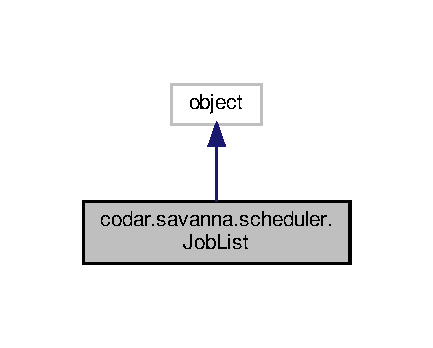
\includegraphics[width=208pt]{classcodar_1_1savanna_1_1scheduler_1_1_job_list__inherit__graph}
\end{center}
\end{figure}


Collaboration diagram for codar.\+savanna.\+scheduler.\+Job\+List\+:
\nopagebreak
\begin{figure}[H]
\begin{center}
\leavevmode
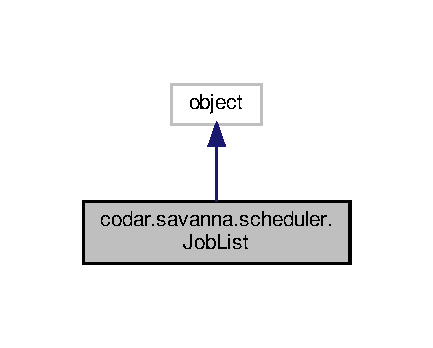
\includegraphics[width=208pt]{classcodar_1_1savanna_1_1scheduler_1_1_job_list__coll__graph}
\end{center}
\end{figure}
\subsection*{Public Member Functions}
\begin{DoxyCompactItemize}
\item 
def \hyperlink{classcodar_1_1savanna_1_1scheduler_1_1_job_list_a692f67c81a57a97d01e899aa1f468435}{\+\_\+\+\_\+init\+\_\+\+\_\+} (self, costfn, initial\+\_\+jobs=None)
\item 
def \hyperlink{classcodar_1_1savanna_1_1scheduler_1_1_job_list_a235fcb4111e178e10fc7ab644bf9b531}{add\+\_\+job} (self, job)
\item 
def \hyperlink{classcodar_1_1savanna_1_1scheduler_1_1_job_list_a5aacbb616928bc7e9078ea08afe8d5ef}{pop\+\_\+job} (self, max\+\_\+cost)
\item 
def \hyperlink{classcodar_1_1savanna_1_1scheduler_1_1_job_list_a2ff2f963962e0c5cf5dac35c3cd37647}{\+\_\+\+\_\+len\+\_\+\+\_\+} (self)
\end{DoxyCompactItemize}


\subsection{Detailed Description}
\begin{DoxyVerb}Manage a job list that can find and remove the highest cost job that
doesn't exceed max_cost and insert new jobs.

The job objects can be any type, but a key function must be provided
that takes an instance of a job and returns it's cost.

Uses a coordinated pair of sort list for costs and jobs, along with
the bisect module. A linked list might be more efficient, since the
list copy on insert and delete may dominate the time to do a linear
search of a small list, but it's likely fine either way for the
sizes we will encounter.\end{DoxyVerb}
 

Definition at line 18 of file scheduler.\+py.



\subsection{Constructor \& Destructor Documentation}
\mbox{\Hypertarget{classcodar_1_1savanna_1_1scheduler_1_1_job_list_a692f67c81a57a97d01e899aa1f468435}\label{classcodar_1_1savanna_1_1scheduler_1_1_job_list_a692f67c81a57a97d01e899aa1f468435}} 
\index{codar\+::savanna\+::scheduler\+::\+Job\+List@{codar\+::savanna\+::scheduler\+::\+Job\+List}!\+\_\+\+\_\+init\+\_\+\+\_\+@{\+\_\+\+\_\+init\+\_\+\+\_\+}}
\index{\+\_\+\+\_\+init\+\_\+\+\_\+@{\+\_\+\+\_\+init\+\_\+\+\_\+}!codar\+::savanna\+::scheduler\+::\+Job\+List@{codar\+::savanna\+::scheduler\+::\+Job\+List}}
\subsubsection{\texorpdfstring{\+\_\+\+\_\+init\+\_\+\+\_\+()}{\_\_init\_\_()}}
{\footnotesize\ttfamily def codar.\+savanna.\+scheduler.\+Job\+List.\+\_\+\+\_\+init\+\_\+\+\_\+ (\begin{DoxyParamCaption}\item[{}]{self,  }\item[{}]{costfn,  }\item[{}]{initial\+\_\+jobs = {\ttfamily None} }\end{DoxyParamCaption})}



Definition at line 30 of file scheduler.\+py.



\subsection{Member Function Documentation}
\mbox{\Hypertarget{classcodar_1_1savanna_1_1scheduler_1_1_job_list_a2ff2f963962e0c5cf5dac35c3cd37647}\label{classcodar_1_1savanna_1_1scheduler_1_1_job_list_a2ff2f963962e0c5cf5dac35c3cd37647}} 
\index{codar\+::savanna\+::scheduler\+::\+Job\+List@{codar\+::savanna\+::scheduler\+::\+Job\+List}!\+\_\+\+\_\+len\+\_\+\+\_\+@{\+\_\+\+\_\+len\+\_\+\+\_\+}}
\index{\+\_\+\+\_\+len\+\_\+\+\_\+@{\+\_\+\+\_\+len\+\_\+\+\_\+}!codar\+::savanna\+::scheduler\+::\+Job\+List@{codar\+::savanna\+::scheduler\+::\+Job\+List}}
\subsubsection{\texorpdfstring{\+\_\+\+\_\+len\+\_\+\+\_\+()}{\_\_len\_\_()}}
{\footnotesize\ttfamily def codar.\+savanna.\+scheduler.\+Job\+List.\+\_\+\+\_\+len\+\_\+\+\_\+ (\begin{DoxyParamCaption}\item[{}]{self }\end{DoxyParamCaption})}



Definition at line 63 of file scheduler.\+py.

\mbox{\Hypertarget{classcodar_1_1savanna_1_1scheduler_1_1_job_list_a235fcb4111e178e10fc7ab644bf9b531}\label{classcodar_1_1savanna_1_1scheduler_1_1_job_list_a235fcb4111e178e10fc7ab644bf9b531}} 
\index{codar\+::savanna\+::scheduler\+::\+Job\+List@{codar\+::savanna\+::scheduler\+::\+Job\+List}!add\+\_\+job@{add\+\_\+job}}
\index{add\+\_\+job@{add\+\_\+job}!codar\+::savanna\+::scheduler\+::\+Job\+List@{codar\+::savanna\+::scheduler\+::\+Job\+List}}
\subsubsection{\texorpdfstring{add\+\_\+job()}{add\_job()}}
{\footnotesize\ttfamily def codar.\+savanna.\+scheduler.\+Job\+List.\+add\+\_\+job (\begin{DoxyParamCaption}\item[{}]{self,  }\item[{}]{job }\end{DoxyParamCaption})}



Definition at line 41 of file scheduler.\+py.

\mbox{\Hypertarget{classcodar_1_1savanna_1_1scheduler_1_1_job_list_a5aacbb616928bc7e9078ea08afe8d5ef}\label{classcodar_1_1savanna_1_1scheduler_1_1_job_list_a5aacbb616928bc7e9078ea08afe8d5ef}} 
\index{codar\+::savanna\+::scheduler\+::\+Job\+List@{codar\+::savanna\+::scheduler\+::\+Job\+List}!pop\+\_\+job@{pop\+\_\+job}}
\index{pop\+\_\+job@{pop\+\_\+job}!codar\+::savanna\+::scheduler\+::\+Job\+List@{codar\+::savanna\+::scheduler\+::\+Job\+List}}
\subsubsection{\texorpdfstring{pop\+\_\+job()}{pop\_job()}}
{\footnotesize\ttfamily def codar.\+savanna.\+scheduler.\+Job\+List.\+pop\+\_\+job (\begin{DoxyParamCaption}\item[{}]{self,  }\item[{}]{max\+\_\+cost }\end{DoxyParamCaption})}

\begin{DoxyVerb}Get the highest cost job that doesn't exceed max_cost, and remove
it from the job list. Raises IndexError if the job list is empty,
returns None if no suitable jobs exist in the list.\end{DoxyVerb}
 

Definition at line 48 of file scheduler.\+py.



The documentation for this class was generated from the following file\+:\begin{DoxyCompactItemize}
\item 
\hyperlink{scheduler_8py}{scheduler.\+py}\end{DoxyCompactItemize}

\hypertarget{classcodar_1_1savanna_1_1producer_1_1_j_s_o_n_file_pipeline_reader}{}\section{codar.\+savanna.\+producer.\+J\+S\+O\+N\+File\+Pipeline\+Reader Class Reference}
\label{classcodar_1_1savanna_1_1producer_1_1_j_s_o_n_file_pipeline_reader}\index{codar.\+savanna.\+producer.\+J\+S\+O\+N\+File\+Pipeline\+Reader@{codar.\+savanna.\+producer.\+J\+S\+O\+N\+File\+Pipeline\+Reader}}


Inheritance diagram for codar.\+savanna.\+producer.\+J\+S\+O\+N\+File\+Pipeline\+Reader\+:
\nopagebreak
\begin{figure}[H]
\begin{center}
\leavevmode
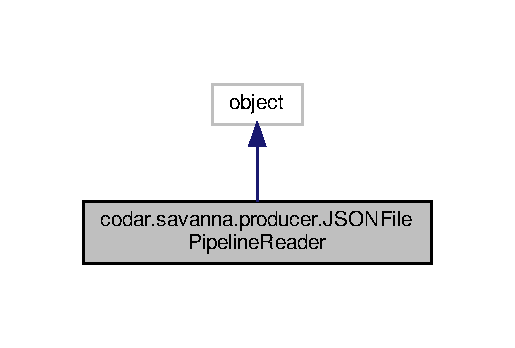
\includegraphics[width=247pt]{classcodar_1_1savanna_1_1producer_1_1_j_s_o_n_file_pipeline_reader__inherit__graph}
\end{center}
\end{figure}


Collaboration diagram for codar.\+savanna.\+producer.\+J\+S\+O\+N\+File\+Pipeline\+Reader\+:
\nopagebreak
\begin{figure}[H]
\begin{center}
\leavevmode
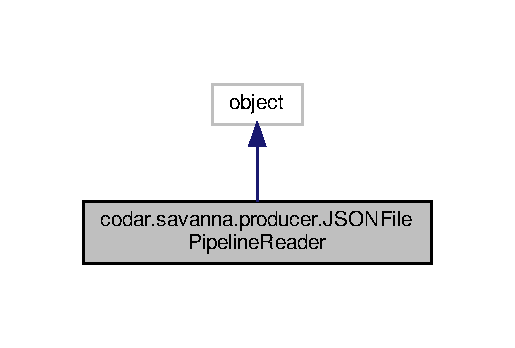
\includegraphics[width=247pt]{classcodar_1_1savanna_1_1producer_1_1_j_s_o_n_file_pipeline_reader__coll__graph}
\end{center}
\end{figure}
\subsection*{Public Member Functions}
\begin{DoxyCompactItemize}
\item 
def \hyperlink{classcodar_1_1savanna_1_1producer_1_1_j_s_o_n_file_pipeline_reader_a55313d819000a60b4c1d0acc6723722b}{\+\_\+\+\_\+init\+\_\+\+\_\+} (self, \hyperlink{classcodar_1_1savanna_1_1producer_1_1_j_s_o_n_file_pipeline_reader_a492f862e3d8692400cc29b11df5cf137}{file\+\_\+path})
\item 
def \hyperlink{classcodar_1_1savanna_1_1producer_1_1_j_s_o_n_file_pipeline_reader_a1b4cf622fdd2146181d5776f044c97c6}{read\+\_\+pipelines} (self)
\end{DoxyCompactItemize}
\subsection*{Public Attributes}
\begin{DoxyCompactItemize}
\item 
\hyperlink{classcodar_1_1savanna_1_1producer_1_1_j_s_o_n_file_pipeline_reader_a492f862e3d8692400cc29b11df5cf137}{file\+\_\+path}
\end{DoxyCompactItemize}


\subsection{Detailed Description}
\begin{DoxyVerb}Load pipelines from a file formatted as a new line separated list of
JSON documents. Each JSON document must be a list containing dictionaries,
each dictionary discribing a code to run as part of the pipeline.\end{DoxyVerb}
 

Definition at line 12 of file producer.\+py.



\subsection{Constructor \& Destructor Documentation}
\mbox{\Hypertarget{classcodar_1_1savanna_1_1producer_1_1_j_s_o_n_file_pipeline_reader_a55313d819000a60b4c1d0acc6723722b}\label{classcodar_1_1savanna_1_1producer_1_1_j_s_o_n_file_pipeline_reader_a55313d819000a60b4c1d0acc6723722b}} 
\index{codar\+::savanna\+::producer\+::\+J\+S\+O\+N\+File\+Pipeline\+Reader@{codar\+::savanna\+::producer\+::\+J\+S\+O\+N\+File\+Pipeline\+Reader}!\+\_\+\+\_\+init\+\_\+\+\_\+@{\+\_\+\+\_\+init\+\_\+\+\_\+}}
\index{\+\_\+\+\_\+init\+\_\+\+\_\+@{\+\_\+\+\_\+init\+\_\+\+\_\+}!codar\+::savanna\+::producer\+::\+J\+S\+O\+N\+File\+Pipeline\+Reader@{codar\+::savanna\+::producer\+::\+J\+S\+O\+N\+File\+Pipeline\+Reader}}
\subsubsection{\texorpdfstring{\+\_\+\+\_\+init\+\_\+\+\_\+()}{\_\_init\_\_()}}
{\footnotesize\ttfamily def codar.\+savanna.\+producer.\+J\+S\+O\+N\+File\+Pipeline\+Reader.\+\_\+\+\_\+init\+\_\+\+\_\+ (\begin{DoxyParamCaption}\item[{}]{self,  }\item[{}]{file\+\_\+path }\end{DoxyParamCaption})}



Definition at line 17 of file producer.\+py.



\subsection{Member Function Documentation}
\mbox{\Hypertarget{classcodar_1_1savanna_1_1producer_1_1_j_s_o_n_file_pipeline_reader_a1b4cf622fdd2146181d5776f044c97c6}\label{classcodar_1_1savanna_1_1producer_1_1_j_s_o_n_file_pipeline_reader_a1b4cf622fdd2146181d5776f044c97c6}} 
\index{codar\+::savanna\+::producer\+::\+J\+S\+O\+N\+File\+Pipeline\+Reader@{codar\+::savanna\+::producer\+::\+J\+S\+O\+N\+File\+Pipeline\+Reader}!read\+\_\+pipelines@{read\+\_\+pipelines}}
\index{read\+\_\+pipelines@{read\+\_\+pipelines}!codar\+::savanna\+::producer\+::\+J\+S\+O\+N\+File\+Pipeline\+Reader@{codar\+::savanna\+::producer\+::\+J\+S\+O\+N\+File\+Pipeline\+Reader}}
\subsubsection{\texorpdfstring{read\+\_\+pipelines()}{read\_pipelines()}}
{\footnotesize\ttfamily def codar.\+savanna.\+producer.\+J\+S\+O\+N\+File\+Pipeline\+Reader.\+read\+\_\+pipelines (\begin{DoxyParamCaption}\item[{}]{self }\end{DoxyParamCaption})}



Definition at line 20 of file producer.\+py.



\subsection{Member Data Documentation}
\mbox{\Hypertarget{classcodar_1_1savanna_1_1producer_1_1_j_s_o_n_file_pipeline_reader_a492f862e3d8692400cc29b11df5cf137}\label{classcodar_1_1savanna_1_1producer_1_1_j_s_o_n_file_pipeline_reader_a492f862e3d8692400cc29b11df5cf137}} 
\index{codar\+::savanna\+::producer\+::\+J\+S\+O\+N\+File\+Pipeline\+Reader@{codar\+::savanna\+::producer\+::\+J\+S\+O\+N\+File\+Pipeline\+Reader}!file\+\_\+path@{file\+\_\+path}}
\index{file\+\_\+path@{file\+\_\+path}!codar\+::savanna\+::producer\+::\+J\+S\+O\+N\+File\+Pipeline\+Reader@{codar\+::savanna\+::producer\+::\+J\+S\+O\+N\+File\+Pipeline\+Reader}}
\subsubsection{\texorpdfstring{file\+\_\+path}{file\_path}}
{\footnotesize\ttfamily codar.\+savanna.\+producer.\+J\+S\+O\+N\+File\+Pipeline\+Reader.\+file\+\_\+path}



Definition at line 18 of file producer.\+py.



The documentation for this class was generated from the following file\+:\begin{DoxyCompactItemize}
\item 
\hyperlink{producer_8py}{producer.\+py}\end{DoxyCompactItemize}

\hypertarget{classcodar_1_1savanna_1_1machines_1_1_machine}{}\section{codar.\+savanna.\+machines.\+Machine Class Reference}
\label{classcodar_1_1savanna_1_1machines_1_1_machine}\index{codar.\+savanna.\+machines.\+Machine@{codar.\+savanna.\+machines.\+Machine}}


Inheritance diagram for codar.\+savanna.\+machines.\+Machine\+:
\nopagebreak
\begin{figure}[H]
\begin{center}
\leavevmode
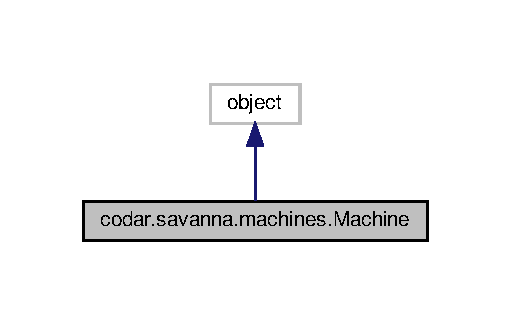
\includegraphics[width=245pt]{classcodar_1_1savanna_1_1machines_1_1_machine__inherit__graph}
\end{center}
\end{figure}


Collaboration diagram for codar.\+savanna.\+machines.\+Machine\+:
\nopagebreak
\begin{figure}[H]
\begin{center}
\leavevmode
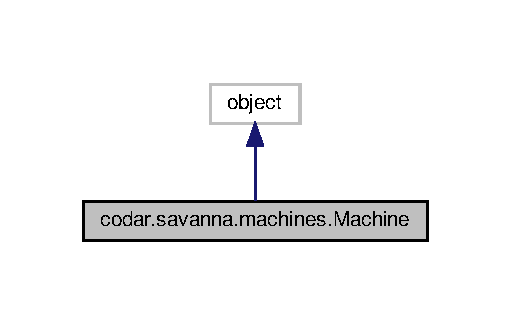
\includegraphics[width=245pt]{classcodar_1_1savanna_1_1machines_1_1_machine__coll__graph}
\end{center}
\end{figure}
\subsection*{Public Member Functions}
\begin{DoxyCompactItemize}
\item 
def \hyperlink{classcodar_1_1savanna_1_1machines_1_1_machine_a604279a4e666c75e59716eefc01be972}{\+\_\+\+\_\+init\+\_\+\+\_\+} (self, \hyperlink{classcodar_1_1savanna_1_1machines_1_1_machine_a7d2164c63e076a7240947b1a70e62f0f}{name}, \hyperlink{classcodar_1_1savanna_1_1machines_1_1_machine_a179ace208a51d849459bf26fcf54acc4}{scheduler\+\_\+name}, \hyperlink{classcodar_1_1savanna_1_1machines_1_1_machine_a65b17faeda10d83fdd8766430d62815f}{runner\+\_\+name}, \hyperlink{classcodar_1_1savanna_1_1machines_1_1_machine_ad1f413ae8607221317675adb19a7887a}{node\+\_\+class}, \hyperlink{classcodar_1_1savanna_1_1machines_1_1_machine_a4b4c0eda863f1003ae7d8bda02f2b96b}{processes\+\_\+per\+\_\+node}=None, \hyperlink{classcodar_1_1savanna_1_1machines_1_1_machine_a516048c489dc334f0fe45d529e59c181}{node\+\_\+exclusive}=False, \hyperlink{classcodar_1_1savanna_1_1machines_1_1_machine_aa26c50a13e89160894eff5a7fb180ed7}{scheduler\+\_\+options}=None, \hyperlink{classcodar_1_1savanna_1_1machines_1_1_machine_a636168243907ca1035c8683a31a69c86}{dataspaces\+\_\+servers\+\_\+per\+\_\+node}=1)
\item 
def \hyperlink{classcodar_1_1savanna_1_1machines_1_1_machine_a50a9259a741eef79d1de2529a9d1f1ae}{get\+\_\+scheduler\+\_\+options} (self, options)
\item 
def \hyperlink{classcodar_1_1savanna_1_1machines_1_1_machine_a13cd507ffb654ef95477f9cd22de6691}{get\+\_\+nodes\+\_\+reqd} (self)
\end{DoxyCompactItemize}
\subsection*{Public Attributes}
\begin{DoxyCompactItemize}
\item 
\hyperlink{classcodar_1_1savanna_1_1machines_1_1_machine_a7d2164c63e076a7240947b1a70e62f0f}{name}
\item 
\hyperlink{classcodar_1_1savanna_1_1machines_1_1_machine_a179ace208a51d849459bf26fcf54acc4}{scheduler\+\_\+name}
\item 
\hyperlink{classcodar_1_1savanna_1_1machines_1_1_machine_a65b17faeda10d83fdd8766430d62815f}{runner\+\_\+name}
\item 
\hyperlink{classcodar_1_1savanna_1_1machines_1_1_machine_ad1f413ae8607221317675adb19a7887a}{node\+\_\+class}
\item 
\hyperlink{classcodar_1_1savanna_1_1machines_1_1_machine_a4b4c0eda863f1003ae7d8bda02f2b96b}{processes\+\_\+per\+\_\+node}
\item 
\hyperlink{classcodar_1_1savanna_1_1machines_1_1_machine_a516048c489dc334f0fe45d529e59c181}{node\+\_\+exclusive}
\item 
\hyperlink{classcodar_1_1savanna_1_1machines_1_1_machine_aa26c50a13e89160894eff5a7fb180ed7}{scheduler\+\_\+options}
\item 
\hyperlink{classcodar_1_1savanna_1_1machines_1_1_machine_a636168243907ca1035c8683a31a69c86}{dataspaces\+\_\+servers\+\_\+per\+\_\+node}
\end{DoxyCompactItemize}


\subsection{Detailed Description}
\begin{DoxyVerb}Class to represent configuration of a specific Supercomputer or
workstation, including the scheduler and runner used by the machine.
This can be used to map an experiment to run on the machine without
having to define machine specific parameter for every experiment
separately.\end{DoxyVerb}
 

Definition at line 69 of file machines.\+py.



\subsection{Constructor \& Destructor Documentation}
\mbox{\Hypertarget{classcodar_1_1savanna_1_1machines_1_1_machine_a604279a4e666c75e59716eefc01be972}\label{classcodar_1_1savanna_1_1machines_1_1_machine_a604279a4e666c75e59716eefc01be972}} 
\index{codar\+::savanna\+::machines\+::\+Machine@{codar\+::savanna\+::machines\+::\+Machine}!\+\_\+\+\_\+init\+\_\+\+\_\+@{\+\_\+\+\_\+init\+\_\+\+\_\+}}
\index{\+\_\+\+\_\+init\+\_\+\+\_\+@{\+\_\+\+\_\+init\+\_\+\+\_\+}!codar\+::savanna\+::machines\+::\+Machine@{codar\+::savanna\+::machines\+::\+Machine}}
\subsubsection{\texorpdfstring{\+\_\+\+\_\+init\+\_\+\+\_\+()}{\_\_init\_\_()}}
{\footnotesize\ttfamily def codar.\+savanna.\+machines.\+Machine.\+\_\+\+\_\+init\+\_\+\+\_\+ (\begin{DoxyParamCaption}\item[{}]{self,  }\item[{}]{name,  }\item[{}]{scheduler\+\_\+name,  }\item[{}]{runner\+\_\+name,  }\item[{}]{node\+\_\+class,  }\item[{}]{processes\+\_\+per\+\_\+node = {\ttfamily None},  }\item[{}]{node\+\_\+exclusive = {\ttfamily False},  }\item[{}]{scheduler\+\_\+options = {\ttfamily None},  }\item[{}]{dataspaces\+\_\+servers\+\_\+per\+\_\+node = {\ttfamily 1} }\end{DoxyParamCaption})}



Definition at line 78 of file machines.\+py.



\subsection{Member Function Documentation}
\mbox{\Hypertarget{classcodar_1_1savanna_1_1machines_1_1_machine_a13cd507ffb654ef95477f9cd22de6691}\label{classcodar_1_1savanna_1_1machines_1_1_machine_a13cd507ffb654ef95477f9cd22de6691}} 
\index{codar\+::savanna\+::machines\+::\+Machine@{codar\+::savanna\+::machines\+::\+Machine}!get\+\_\+nodes\+\_\+reqd@{get\+\_\+nodes\+\_\+reqd}}
\index{get\+\_\+nodes\+\_\+reqd@{get\+\_\+nodes\+\_\+reqd}!codar\+::savanna\+::machines\+::\+Machine@{codar\+::savanna\+::machines\+::\+Machine}}
\subsubsection{\texorpdfstring{get\+\_\+nodes\+\_\+reqd()}{get\_nodes\_reqd()}}
{\footnotesize\ttfamily def codar.\+savanna.\+machines.\+Machine.\+get\+\_\+nodes\+\_\+reqd (\begin{DoxyParamCaption}\item[{}]{self }\end{DoxyParamCaption})}



Definition at line 100 of file machines.\+py.

\mbox{\Hypertarget{classcodar_1_1savanna_1_1machines_1_1_machine_a50a9259a741eef79d1de2529a9d1f1ae}\label{classcodar_1_1savanna_1_1machines_1_1_machine_a50a9259a741eef79d1de2529a9d1f1ae}} 
\index{codar\+::savanna\+::machines\+::\+Machine@{codar\+::savanna\+::machines\+::\+Machine}!get\+\_\+scheduler\+\_\+options@{get\+\_\+scheduler\+\_\+options}}
\index{get\+\_\+scheduler\+\_\+options@{get\+\_\+scheduler\+\_\+options}!codar\+::savanna\+::machines\+::\+Machine@{codar\+::savanna\+::machines\+::\+Machine}}
\subsubsection{\texorpdfstring{get\+\_\+scheduler\+\_\+options()}{get\_scheduler\_options()}}
{\footnotesize\ttfamily def codar.\+savanna.\+machines.\+Machine.\+get\+\_\+scheduler\+\_\+options (\begin{DoxyParamCaption}\item[{}]{self,  }\item[{}]{options }\end{DoxyParamCaption})}

\begin{DoxyVerb}Validate supplied options and add default values where missing.
Returns a new dictionary.\end{DoxyVerb}
 

Definition at line 91 of file machines.\+py.



\subsection{Member Data Documentation}
\mbox{\Hypertarget{classcodar_1_1savanna_1_1machines_1_1_machine_a636168243907ca1035c8683a31a69c86}\label{classcodar_1_1savanna_1_1machines_1_1_machine_a636168243907ca1035c8683a31a69c86}} 
\index{codar\+::savanna\+::machines\+::\+Machine@{codar\+::savanna\+::machines\+::\+Machine}!dataspaces\+\_\+servers\+\_\+per\+\_\+node@{dataspaces\+\_\+servers\+\_\+per\+\_\+node}}
\index{dataspaces\+\_\+servers\+\_\+per\+\_\+node@{dataspaces\+\_\+servers\+\_\+per\+\_\+node}!codar\+::savanna\+::machines\+::\+Machine@{codar\+::savanna\+::machines\+::\+Machine}}
\subsubsection{\texorpdfstring{dataspaces\+\_\+servers\+\_\+per\+\_\+node}{dataspaces\_servers\_per\_node}}
{\footnotesize\ttfamily codar.\+savanna.\+machines.\+Machine.\+dataspaces\+\_\+servers\+\_\+per\+\_\+node}



Definition at line 89 of file machines.\+py.

\mbox{\Hypertarget{classcodar_1_1savanna_1_1machines_1_1_machine_a7d2164c63e076a7240947b1a70e62f0f}\label{classcodar_1_1savanna_1_1machines_1_1_machine_a7d2164c63e076a7240947b1a70e62f0f}} 
\index{codar\+::savanna\+::machines\+::\+Machine@{codar\+::savanna\+::machines\+::\+Machine}!name@{name}}
\index{name@{name}!codar\+::savanna\+::machines\+::\+Machine@{codar\+::savanna\+::machines\+::\+Machine}}
\subsubsection{\texorpdfstring{name}{name}}
{\footnotesize\ttfamily codar.\+savanna.\+machines.\+Machine.\+name}



Definition at line 79 of file machines.\+py.

\mbox{\Hypertarget{classcodar_1_1savanna_1_1machines_1_1_machine_ad1f413ae8607221317675adb19a7887a}\label{classcodar_1_1savanna_1_1machines_1_1_machine_ad1f413ae8607221317675adb19a7887a}} 
\index{codar\+::savanna\+::machines\+::\+Machine@{codar\+::savanna\+::machines\+::\+Machine}!node\+\_\+class@{node\+\_\+class}}
\index{node\+\_\+class@{node\+\_\+class}!codar\+::savanna\+::machines\+::\+Machine@{codar\+::savanna\+::machines\+::\+Machine}}
\subsubsection{\texorpdfstring{node\+\_\+class}{node\_class}}
{\footnotesize\ttfamily codar.\+savanna.\+machines.\+Machine.\+node\+\_\+class}



Definition at line 82 of file machines.\+py.

\mbox{\Hypertarget{classcodar_1_1savanna_1_1machines_1_1_machine_a516048c489dc334f0fe45d529e59c181}\label{classcodar_1_1savanna_1_1machines_1_1_machine_a516048c489dc334f0fe45d529e59c181}} 
\index{codar\+::savanna\+::machines\+::\+Machine@{codar\+::savanna\+::machines\+::\+Machine}!node\+\_\+exclusive@{node\+\_\+exclusive}}
\index{node\+\_\+exclusive@{node\+\_\+exclusive}!codar\+::savanna\+::machines\+::\+Machine@{codar\+::savanna\+::machines\+::\+Machine}}
\subsubsection{\texorpdfstring{node\+\_\+exclusive}{node\_exclusive}}
{\footnotesize\ttfamily codar.\+savanna.\+machines.\+Machine.\+node\+\_\+exclusive}



Definition at line 86 of file machines.\+py.

\mbox{\Hypertarget{classcodar_1_1savanna_1_1machines_1_1_machine_a4b4c0eda863f1003ae7d8bda02f2b96b}\label{classcodar_1_1savanna_1_1machines_1_1_machine_a4b4c0eda863f1003ae7d8bda02f2b96b}} 
\index{codar\+::savanna\+::machines\+::\+Machine@{codar\+::savanna\+::machines\+::\+Machine}!processes\+\_\+per\+\_\+node@{processes\+\_\+per\+\_\+node}}
\index{processes\+\_\+per\+\_\+node@{processes\+\_\+per\+\_\+node}!codar\+::savanna\+::machines\+::\+Machine@{codar\+::savanna\+::machines\+::\+Machine}}
\subsubsection{\texorpdfstring{processes\+\_\+per\+\_\+node}{processes\_per\_node}}
{\footnotesize\ttfamily codar.\+savanna.\+machines.\+Machine.\+processes\+\_\+per\+\_\+node}



Definition at line 85 of file machines.\+py.

\mbox{\Hypertarget{classcodar_1_1savanna_1_1machines_1_1_machine_a65b17faeda10d83fdd8766430d62815f}\label{classcodar_1_1savanna_1_1machines_1_1_machine_a65b17faeda10d83fdd8766430d62815f}} 
\index{codar\+::savanna\+::machines\+::\+Machine@{codar\+::savanna\+::machines\+::\+Machine}!runner\+\_\+name@{runner\+\_\+name}}
\index{runner\+\_\+name@{runner\+\_\+name}!codar\+::savanna\+::machines\+::\+Machine@{codar\+::savanna\+::machines\+::\+Machine}}
\subsubsection{\texorpdfstring{runner\+\_\+name}{runner\_name}}
{\footnotesize\ttfamily codar.\+savanna.\+machines.\+Machine.\+runner\+\_\+name}



Definition at line 81 of file machines.\+py.

\mbox{\Hypertarget{classcodar_1_1savanna_1_1machines_1_1_machine_a179ace208a51d849459bf26fcf54acc4}\label{classcodar_1_1savanna_1_1machines_1_1_machine_a179ace208a51d849459bf26fcf54acc4}} 
\index{codar\+::savanna\+::machines\+::\+Machine@{codar\+::savanna\+::machines\+::\+Machine}!scheduler\+\_\+name@{scheduler\+\_\+name}}
\index{scheduler\+\_\+name@{scheduler\+\_\+name}!codar\+::savanna\+::machines\+::\+Machine@{codar\+::savanna\+::machines\+::\+Machine}}
\subsubsection{\texorpdfstring{scheduler\+\_\+name}{scheduler\_name}}
{\footnotesize\ttfamily codar.\+savanna.\+machines.\+Machine.\+scheduler\+\_\+name}



Definition at line 80 of file machines.\+py.

\mbox{\Hypertarget{classcodar_1_1savanna_1_1machines_1_1_machine_aa26c50a13e89160894eff5a7fb180ed7}\label{classcodar_1_1savanna_1_1machines_1_1_machine_aa26c50a13e89160894eff5a7fb180ed7}} 
\index{codar\+::savanna\+::machines\+::\+Machine@{codar\+::savanna\+::machines\+::\+Machine}!scheduler\+\_\+options@{scheduler\+\_\+options}}
\index{scheduler\+\_\+options@{scheduler\+\_\+options}!codar\+::savanna\+::machines\+::\+Machine@{codar\+::savanna\+::machines\+::\+Machine}}
\subsubsection{\texorpdfstring{scheduler\+\_\+options}{scheduler\_options}}
{\footnotesize\ttfamily codar.\+savanna.\+machines.\+Machine.\+scheduler\+\_\+options}



Definition at line 88 of file machines.\+py.



The documentation for this class was generated from the following file\+:\begin{DoxyCompactItemize}
\item 
savanna/\hyperlink{machines_8py}{machines.\+py}\end{DoxyCompactItemize}

\hypertarget{classcodar_1_1savanna_1_1machines_1_1_machine_node}{}\section{codar.\+savanna.\+machines.\+Machine\+Node Class Reference}
\label{classcodar_1_1savanna_1_1machines_1_1_machine_node}\index{codar.\+savanna.\+machines.\+Machine\+Node@{codar.\+savanna.\+machines.\+Machine\+Node}}


Inheritance diagram for codar.\+savanna.\+machines.\+Machine\+Node\+:
\nopagebreak
\begin{figure}[H]
\begin{center}
\leavevmode
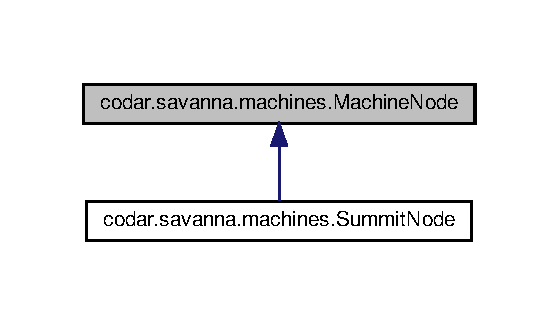
\includegraphics[width=268pt]{classcodar_1_1savanna_1_1machines_1_1_machine_node__inherit__graph}
\end{center}
\end{figure}
\subsection*{Public Member Functions}
\begin{DoxyCompactItemize}
\item 
def \hyperlink{classcodar_1_1savanna_1_1machines_1_1_machine_node_adc12f9810d54e9f497a4df2c3ab80577}{\+\_\+\+\_\+init\+\_\+\+\_\+} (self, num\+\_\+cpus, num\+\_\+gpus)
\item 
def \hyperlink{classcodar_1_1savanna_1_1machines_1_1_machine_node_a32ee6eb242c8dff720e89ffbd772cf40}{validate\+\_\+layout} (self)
\item 
def \hyperlink{classcodar_1_1savanna_1_1machines_1_1_machine_node_a9598980dfb90152c1f2091fae5dd1299}{to\+\_\+json} (self)
\end{DoxyCompactItemize}
\subsection*{Public Attributes}
\begin{DoxyCompactItemize}
\item 
\hyperlink{classcodar_1_1savanna_1_1machines_1_1_machine_node_a084bb8daed740edd8b7dd37f8d1f9bab}{cpu}
\item 
\hyperlink{classcodar_1_1savanna_1_1machines_1_1_machine_node_a2ccec1288c1472fc0a5af7787e48da22}{gpu}
\end{DoxyCompactItemize}


\subsection{Detailed Description}


Definition at line 16 of file machines.\+py.



\subsection{Constructor \& Destructor Documentation}
\mbox{\Hypertarget{classcodar_1_1savanna_1_1machines_1_1_machine_node_adc12f9810d54e9f497a4df2c3ab80577}\label{classcodar_1_1savanna_1_1machines_1_1_machine_node_adc12f9810d54e9f497a4df2c3ab80577}} 
\index{codar\+::savanna\+::machines\+::\+Machine\+Node@{codar\+::savanna\+::machines\+::\+Machine\+Node}!\+\_\+\+\_\+init\+\_\+\+\_\+@{\+\_\+\+\_\+init\+\_\+\+\_\+}}
\index{\+\_\+\+\_\+init\+\_\+\+\_\+@{\+\_\+\+\_\+init\+\_\+\+\_\+}!codar\+::savanna\+::machines\+::\+Machine\+Node@{codar\+::savanna\+::machines\+::\+Machine\+Node}}
\subsubsection{\texorpdfstring{\+\_\+\+\_\+init\+\_\+\+\_\+()}{\_\_init\_\_()}}
{\footnotesize\ttfamily def codar.\+savanna.\+machines.\+Machine\+Node.\+\_\+\+\_\+init\+\_\+\+\_\+ (\begin{DoxyParamCaption}\item[{}]{self,  }\item[{}]{num\+\_\+cpus,  }\item[{}]{num\+\_\+gpus }\end{DoxyParamCaption})}



Definition at line 17 of file machines.\+py.



\subsection{Member Function Documentation}
\mbox{\Hypertarget{classcodar_1_1savanna_1_1machines_1_1_machine_node_a9598980dfb90152c1f2091fae5dd1299}\label{classcodar_1_1savanna_1_1machines_1_1_machine_node_a9598980dfb90152c1f2091fae5dd1299}} 
\index{codar\+::savanna\+::machines\+::\+Machine\+Node@{codar\+::savanna\+::machines\+::\+Machine\+Node}!to\+\_\+json@{to\+\_\+json}}
\index{to\+\_\+json@{to\+\_\+json}!codar\+::savanna\+::machines\+::\+Machine\+Node@{codar\+::savanna\+::machines\+::\+Machine\+Node}}
\subsubsection{\texorpdfstring{to\+\_\+json()}{to\_json()}}
{\footnotesize\ttfamily def codar.\+savanna.\+machines.\+Machine\+Node.\+to\+\_\+json (\begin{DoxyParamCaption}\item[{}]{self }\end{DoxyParamCaption})}



Definition at line 25 of file machines.\+py.

\mbox{\Hypertarget{classcodar_1_1savanna_1_1machines_1_1_machine_node_a32ee6eb242c8dff720e89ffbd772cf40}\label{classcodar_1_1savanna_1_1machines_1_1_machine_node_a32ee6eb242c8dff720e89ffbd772cf40}} 
\index{codar\+::savanna\+::machines\+::\+Machine\+Node@{codar\+::savanna\+::machines\+::\+Machine\+Node}!validate\+\_\+layout@{validate\+\_\+layout}}
\index{validate\+\_\+layout@{validate\+\_\+layout}!codar\+::savanna\+::machines\+::\+Machine\+Node@{codar\+::savanna\+::machines\+::\+Machine\+Node}}
\subsubsection{\texorpdfstring{validate\+\_\+layout()}{validate\_layout()}}
{\footnotesize\ttfamily def codar.\+savanna.\+machines.\+Machine\+Node.\+validate\+\_\+layout (\begin{DoxyParamCaption}\item[{}]{self }\end{DoxyParamCaption})}



Definition at line 22 of file machines.\+py.



\subsection{Member Data Documentation}
\mbox{\Hypertarget{classcodar_1_1savanna_1_1machines_1_1_machine_node_a084bb8daed740edd8b7dd37f8d1f9bab}\label{classcodar_1_1savanna_1_1machines_1_1_machine_node_a084bb8daed740edd8b7dd37f8d1f9bab}} 
\index{codar\+::savanna\+::machines\+::\+Machine\+Node@{codar\+::savanna\+::machines\+::\+Machine\+Node}!cpu@{cpu}}
\index{cpu@{cpu}!codar\+::savanna\+::machines\+::\+Machine\+Node@{codar\+::savanna\+::machines\+::\+Machine\+Node}}
\subsubsection{\texorpdfstring{cpu}{cpu}}
{\footnotesize\ttfamily codar.\+savanna.\+machines.\+Machine\+Node.\+cpu}



Definition at line 19 of file machines.\+py.

\mbox{\Hypertarget{classcodar_1_1savanna_1_1machines_1_1_machine_node_a2ccec1288c1472fc0a5af7787e48da22}\label{classcodar_1_1savanna_1_1machines_1_1_machine_node_a2ccec1288c1472fc0a5af7787e48da22}} 
\index{codar\+::savanna\+::machines\+::\+Machine\+Node@{codar\+::savanna\+::machines\+::\+Machine\+Node}!gpu@{gpu}}
\index{gpu@{gpu}!codar\+::savanna\+::machines\+::\+Machine\+Node@{codar\+::savanna\+::machines\+::\+Machine\+Node}}
\subsubsection{\texorpdfstring{gpu}{gpu}}
{\footnotesize\ttfamily codar.\+savanna.\+machines.\+Machine\+Node.\+gpu}



Definition at line 20 of file machines.\+py.



The documentation for this class was generated from the following file\+:\begin{DoxyCompactItemize}
\item 
savanna/\hyperlink{machines_8py}{machines.\+py}\end{DoxyCompactItemize}

\hypertarget{classcodar_1_1savanna_1_1exc_1_1_machine_not_found}{}\section{codar.\+savanna.\+exc.\+Machine\+Not\+Found Class Reference}
\label{classcodar_1_1savanna_1_1exc_1_1_machine_not_found}\index{codar.\+savanna.\+exc.\+Machine\+Not\+Found@{codar.\+savanna.\+exc.\+Machine\+Not\+Found}}


Inheritance diagram for codar.\+savanna.\+exc.\+Machine\+Not\+Found\+:
\nopagebreak
\begin{figure}[H]
\begin{center}
\leavevmode
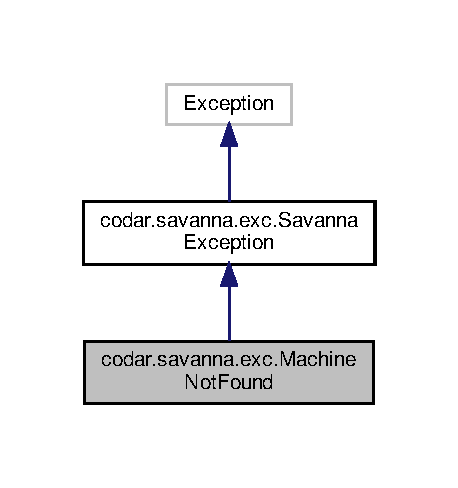
\includegraphics[width=220pt]{classcodar_1_1savanna_1_1exc_1_1_machine_not_found__inherit__graph}
\end{center}
\end{figure}


Collaboration diagram for codar.\+savanna.\+exc.\+Machine\+Not\+Found\+:
\nopagebreak
\begin{figure}[H]
\begin{center}
\leavevmode
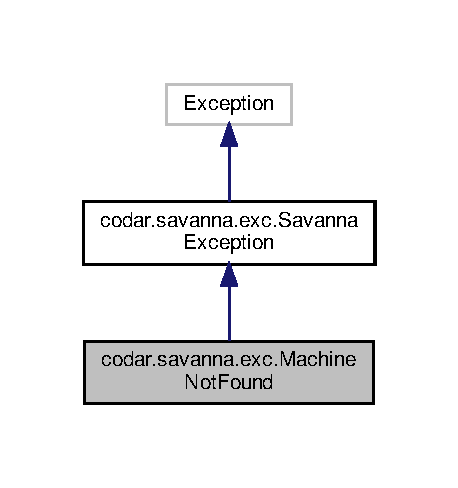
\includegraphics[width=220pt]{classcodar_1_1savanna_1_1exc_1_1_machine_not_found__coll__graph}
\end{center}
\end{figure}
\subsection*{Public Member Functions}
\begin{DoxyCompactItemize}
\item 
def \hyperlink{classcodar_1_1savanna_1_1exc_1_1_machine_not_found_aac59d9a2636166df83d3260fb7bc8933}{\+\_\+\+\_\+init\+\_\+\+\_\+} (self, machine\+\_\+name)
\end{DoxyCompactItemize}


\subsection{Detailed Description}


Definition at line 10 of file exc.\+py.



\subsection{Constructor \& Destructor Documentation}
\mbox{\Hypertarget{classcodar_1_1savanna_1_1exc_1_1_machine_not_found_aac59d9a2636166df83d3260fb7bc8933}\label{classcodar_1_1savanna_1_1exc_1_1_machine_not_found_aac59d9a2636166df83d3260fb7bc8933}} 
\index{codar\+::savanna\+::exc\+::\+Machine\+Not\+Found@{codar\+::savanna\+::exc\+::\+Machine\+Not\+Found}!\+\_\+\+\_\+init\+\_\+\+\_\+@{\+\_\+\+\_\+init\+\_\+\+\_\+}}
\index{\+\_\+\+\_\+init\+\_\+\+\_\+@{\+\_\+\+\_\+init\+\_\+\+\_\+}!codar\+::savanna\+::exc\+::\+Machine\+Not\+Found@{codar\+::savanna\+::exc\+::\+Machine\+Not\+Found}}
\subsubsection{\texorpdfstring{\+\_\+\+\_\+init\+\_\+\+\_\+()}{\_\_init\_\_()}}
{\footnotesize\ttfamily def codar.\+savanna.\+exc.\+Machine\+Not\+Found.\+\_\+\+\_\+init\+\_\+\+\_\+ (\begin{DoxyParamCaption}\item[{}]{self,  }\item[{}]{machine\+\_\+name }\end{DoxyParamCaption})}



Definition at line 11 of file exc.\+py.



The documentation for this class was generated from the following file\+:\begin{DoxyCompactItemize}
\item 
\hyperlink{exc_8py}{exc.\+py}\end{DoxyCompactItemize}

\hypertarget{classcodar_1_1savanna_1_1runners_1_1_m_p_i_runner}{}\section{codar.\+savanna.\+runners.\+M\+P\+I\+Runner Class Reference}
\label{classcodar_1_1savanna_1_1runners_1_1_m_p_i_runner}\index{codar.\+savanna.\+runners.\+M\+P\+I\+Runner@{codar.\+savanna.\+runners.\+M\+P\+I\+Runner}}


Inheritance diagram for codar.\+savanna.\+runners.\+M\+P\+I\+Runner\+:
\nopagebreak
\begin{figure}[H]
\begin{center}
\leavevmode
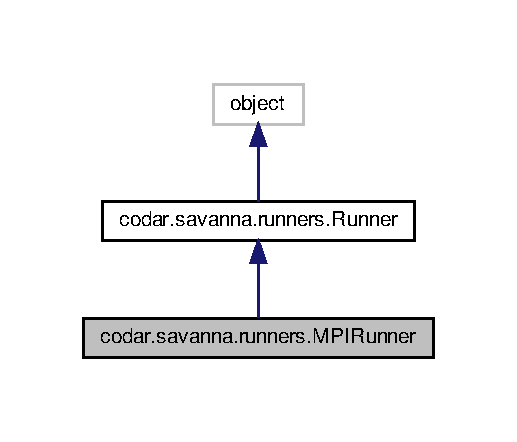
\includegraphics[width=248pt]{classcodar_1_1savanna_1_1runners_1_1_m_p_i_runner__inherit__graph}
\end{center}
\end{figure}


Collaboration diagram for codar.\+savanna.\+runners.\+M\+P\+I\+Runner\+:
\nopagebreak
\begin{figure}[H]
\begin{center}
\leavevmode
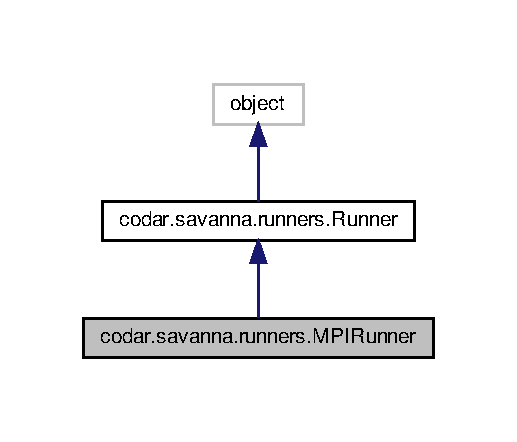
\includegraphics[width=248pt]{classcodar_1_1savanna_1_1runners_1_1_m_p_i_runner__coll__graph}
\end{center}
\end{figure}
\subsection*{Public Member Functions}
\begin{DoxyCompactItemize}
\item 
def \hyperlink{classcodar_1_1savanna_1_1runners_1_1_m_p_i_runner_a67662602e1fe9901e20e17a9f16b8259}{\+\_\+\+\_\+init\+\_\+\+\_\+} (self, \hyperlink{classcodar_1_1savanna_1_1runners_1_1_m_p_i_runner_a7ccd767eb30cbd555f387e5b4d781ffa}{exe}, \hyperlink{classcodar_1_1savanna_1_1runners_1_1_m_p_i_runner_aafcba954932f2160d43e820cf3abe6e1}{nprocs\+\_\+arg}, \hyperlink{classcodar_1_1savanna_1_1runners_1_1_m_p_i_runner_ad139718b16183bd45520e166d6d2b9b9}{nodes\+\_\+arg}=None, \hyperlink{classcodar_1_1savanna_1_1runners_1_1_m_p_i_runner_a58bd05be3e876f5a8f2522262ba934f7}{tasks\+\_\+per\+\_\+node\+\_\+arg}=None, \hyperlink{classcodar_1_1savanna_1_1runners_1_1_m_p_i_runner_ad36885eab0821c149e8798ffbf567af4}{hostfile}=None)
\item 
def \hyperlink{classcodar_1_1savanna_1_1runners_1_1_m_p_i_runner_a2eb86e6b8495ecf2361dc58e4b05c7c5}{wrap} (self, run, sched\+\_\+args, find\+\_\+in\+\_\+path=True)
\end{DoxyCompactItemize}
\subsection*{Public Attributes}
\begin{DoxyCompactItemize}
\item 
\hyperlink{classcodar_1_1savanna_1_1runners_1_1_m_p_i_runner_a7ccd767eb30cbd555f387e5b4d781ffa}{exe}
\item 
\hyperlink{classcodar_1_1savanna_1_1runners_1_1_m_p_i_runner_aafcba954932f2160d43e820cf3abe6e1}{nprocs\+\_\+arg}
\item 
\hyperlink{classcodar_1_1savanna_1_1runners_1_1_m_p_i_runner_ad139718b16183bd45520e166d6d2b9b9}{nodes\+\_\+arg}
\item 
\hyperlink{classcodar_1_1savanna_1_1runners_1_1_m_p_i_runner_a58bd05be3e876f5a8f2522262ba934f7}{tasks\+\_\+per\+\_\+node\+\_\+arg}
\item 
\hyperlink{classcodar_1_1savanna_1_1runners_1_1_m_p_i_runner_ad36885eab0821c149e8798ffbf567af4}{hostfile}
\end{DoxyCompactItemize}


\subsection{Detailed Description}


Definition at line 11 of file runners.\+py.



\subsection{Constructor \& Destructor Documentation}
\mbox{\Hypertarget{classcodar_1_1savanna_1_1runners_1_1_m_p_i_runner_a67662602e1fe9901e20e17a9f16b8259}\label{classcodar_1_1savanna_1_1runners_1_1_m_p_i_runner_a67662602e1fe9901e20e17a9f16b8259}} 
\index{codar\+::savanna\+::runners\+::\+M\+P\+I\+Runner@{codar\+::savanna\+::runners\+::\+M\+P\+I\+Runner}!\+\_\+\+\_\+init\+\_\+\+\_\+@{\+\_\+\+\_\+init\+\_\+\+\_\+}}
\index{\+\_\+\+\_\+init\+\_\+\+\_\+@{\+\_\+\+\_\+init\+\_\+\+\_\+}!codar\+::savanna\+::runners\+::\+M\+P\+I\+Runner@{codar\+::savanna\+::runners\+::\+M\+P\+I\+Runner}}
\subsubsection{\texorpdfstring{\+\_\+\+\_\+init\+\_\+\+\_\+()}{\_\_init\_\_()}}
{\footnotesize\ttfamily def codar.\+savanna.\+runners.\+M\+P\+I\+Runner.\+\_\+\+\_\+init\+\_\+\+\_\+ (\begin{DoxyParamCaption}\item[{}]{self,  }\item[{}]{exe,  }\item[{}]{nprocs\+\_\+arg,  }\item[{}]{nodes\+\_\+arg = {\ttfamily None},  }\item[{}]{tasks\+\_\+per\+\_\+node\+\_\+arg = {\ttfamily None},  }\item[{}]{hostfile = {\ttfamily None} }\end{DoxyParamCaption})}



Definition at line 13 of file runners.\+py.



\subsection{Member Function Documentation}
\mbox{\Hypertarget{classcodar_1_1savanna_1_1runners_1_1_m_p_i_runner_a2eb86e6b8495ecf2361dc58e4b05c7c5}\label{classcodar_1_1savanna_1_1runners_1_1_m_p_i_runner_a2eb86e6b8495ecf2361dc58e4b05c7c5}} 
\index{codar\+::savanna\+::runners\+::\+M\+P\+I\+Runner@{codar\+::savanna\+::runners\+::\+M\+P\+I\+Runner}!wrap@{wrap}}
\index{wrap@{wrap}!codar\+::savanna\+::runners\+::\+M\+P\+I\+Runner@{codar\+::savanna\+::runners\+::\+M\+P\+I\+Runner}}
\subsubsection{\texorpdfstring{wrap()}{wrap()}}
{\footnotesize\ttfamily def codar.\+savanna.\+runners.\+M\+P\+I\+Runner.\+wrap (\begin{DoxyParamCaption}\item[{}]{self,  }\item[{}]{run,  }\item[{}]{sched\+\_\+args,  }\item[{}]{find\+\_\+in\+\_\+path = {\ttfamily True} }\end{DoxyParamCaption})}



Definition at line 20 of file runners.\+py.



\subsection{Member Data Documentation}
\mbox{\Hypertarget{classcodar_1_1savanna_1_1runners_1_1_m_p_i_runner_a7ccd767eb30cbd555f387e5b4d781ffa}\label{classcodar_1_1savanna_1_1runners_1_1_m_p_i_runner_a7ccd767eb30cbd555f387e5b4d781ffa}} 
\index{codar\+::savanna\+::runners\+::\+M\+P\+I\+Runner@{codar\+::savanna\+::runners\+::\+M\+P\+I\+Runner}!exe@{exe}}
\index{exe@{exe}!codar\+::savanna\+::runners\+::\+M\+P\+I\+Runner@{codar\+::savanna\+::runners\+::\+M\+P\+I\+Runner}}
\subsubsection{\texorpdfstring{exe}{exe}}
{\footnotesize\ttfamily codar.\+savanna.\+runners.\+M\+P\+I\+Runner.\+exe}



Definition at line 14 of file runners.\+py.

\mbox{\Hypertarget{classcodar_1_1savanna_1_1runners_1_1_m_p_i_runner_ad36885eab0821c149e8798ffbf567af4}\label{classcodar_1_1savanna_1_1runners_1_1_m_p_i_runner_ad36885eab0821c149e8798ffbf567af4}} 
\index{codar\+::savanna\+::runners\+::\+M\+P\+I\+Runner@{codar\+::savanna\+::runners\+::\+M\+P\+I\+Runner}!hostfile@{hostfile}}
\index{hostfile@{hostfile}!codar\+::savanna\+::runners\+::\+M\+P\+I\+Runner@{codar\+::savanna\+::runners\+::\+M\+P\+I\+Runner}}
\subsubsection{\texorpdfstring{hostfile}{hostfile}}
{\footnotesize\ttfamily codar.\+savanna.\+runners.\+M\+P\+I\+Runner.\+hostfile}



Definition at line 18 of file runners.\+py.

\mbox{\Hypertarget{classcodar_1_1savanna_1_1runners_1_1_m_p_i_runner_ad139718b16183bd45520e166d6d2b9b9}\label{classcodar_1_1savanna_1_1runners_1_1_m_p_i_runner_ad139718b16183bd45520e166d6d2b9b9}} 
\index{codar\+::savanna\+::runners\+::\+M\+P\+I\+Runner@{codar\+::savanna\+::runners\+::\+M\+P\+I\+Runner}!nodes\+\_\+arg@{nodes\+\_\+arg}}
\index{nodes\+\_\+arg@{nodes\+\_\+arg}!codar\+::savanna\+::runners\+::\+M\+P\+I\+Runner@{codar\+::savanna\+::runners\+::\+M\+P\+I\+Runner}}
\subsubsection{\texorpdfstring{nodes\+\_\+arg}{nodes\_arg}}
{\footnotesize\ttfamily codar.\+savanna.\+runners.\+M\+P\+I\+Runner.\+nodes\+\_\+arg}



Definition at line 16 of file runners.\+py.

\mbox{\Hypertarget{classcodar_1_1savanna_1_1runners_1_1_m_p_i_runner_aafcba954932f2160d43e820cf3abe6e1}\label{classcodar_1_1savanna_1_1runners_1_1_m_p_i_runner_aafcba954932f2160d43e820cf3abe6e1}} 
\index{codar\+::savanna\+::runners\+::\+M\+P\+I\+Runner@{codar\+::savanna\+::runners\+::\+M\+P\+I\+Runner}!nprocs\+\_\+arg@{nprocs\+\_\+arg}}
\index{nprocs\+\_\+arg@{nprocs\+\_\+arg}!codar\+::savanna\+::runners\+::\+M\+P\+I\+Runner@{codar\+::savanna\+::runners\+::\+M\+P\+I\+Runner}}
\subsubsection{\texorpdfstring{nprocs\+\_\+arg}{nprocs\_arg}}
{\footnotesize\ttfamily codar.\+savanna.\+runners.\+M\+P\+I\+Runner.\+nprocs\+\_\+arg}



Definition at line 15 of file runners.\+py.

\mbox{\Hypertarget{classcodar_1_1savanna_1_1runners_1_1_m_p_i_runner_a58bd05be3e876f5a8f2522262ba934f7}\label{classcodar_1_1savanna_1_1runners_1_1_m_p_i_runner_a58bd05be3e876f5a8f2522262ba934f7}} 
\index{codar\+::savanna\+::runners\+::\+M\+P\+I\+Runner@{codar\+::savanna\+::runners\+::\+M\+P\+I\+Runner}!tasks\+\_\+per\+\_\+node\+\_\+arg@{tasks\+\_\+per\+\_\+node\+\_\+arg}}
\index{tasks\+\_\+per\+\_\+node\+\_\+arg@{tasks\+\_\+per\+\_\+node\+\_\+arg}!codar\+::savanna\+::runners\+::\+M\+P\+I\+Runner@{codar\+::savanna\+::runners\+::\+M\+P\+I\+Runner}}
\subsubsection{\texorpdfstring{tasks\+\_\+per\+\_\+node\+\_\+arg}{tasks\_per\_node\_arg}}
{\footnotesize\ttfamily codar.\+savanna.\+runners.\+M\+P\+I\+Runner.\+tasks\+\_\+per\+\_\+node\+\_\+arg}



Definition at line 17 of file runners.\+py.



The documentation for this class was generated from the following file\+:\begin{DoxyCompactItemize}
\item 
savanna/\hyperlink{savanna_2runners_8py}{runners.\+py}\end{DoxyCompactItemize}

\hypertarget{classcodar_1_1savanna_1_1model_1_1_node_config}{}\section{codar.\+savanna.\+model.\+Node\+Config Class Reference}
\label{classcodar_1_1savanna_1_1model_1_1_node_config}\index{codar.\+savanna.\+model.\+Node\+Config@{codar.\+savanna.\+model.\+Node\+Config}}
\subsection*{Public Member Functions}
\begin{DoxyCompactItemize}
\item 
def \hyperlink{classcodar_1_1savanna_1_1model_1_1_node_config_ad1fad3d3d97b1683dd4d28f77836a002}{\+\_\+\+\_\+init\+\_\+\+\_\+} (self)
\end{DoxyCompactItemize}
\subsection*{Public Attributes}
\begin{DoxyCompactItemize}
\item 
\mbox{\Hypertarget{classcodar_1_1savanna_1_1model_1_1_node_config_abfaac776b1cc5d4b0e6b3dd9d57a32be}\label{classcodar_1_1savanna_1_1model_1_1_node_config_abfaac776b1cc5d4b0e6b3dd9d57a32be}} 
{\bfseries num\+\_\+ranks\+\_\+per\+\_\+node}
\item 
\mbox{\Hypertarget{classcodar_1_1savanna_1_1model_1_1_node_config_ae3b3d48cf476cc01128973780c9ca256}\label{classcodar_1_1savanna_1_1model_1_1_node_config_ae3b3d48cf476cc01128973780c9ca256}} 
{\bfseries cpu}
\item 
\mbox{\Hypertarget{classcodar_1_1savanna_1_1model_1_1_node_config_a073c4acfc108df407fbd8ce570bade6b}\label{classcodar_1_1savanna_1_1model_1_1_node_config_a073c4acfc108df407fbd8ce570bade6b}} 
{\bfseries gpu}
\end{DoxyCompactItemize}


\subsection{Constructor \& Destructor Documentation}
\mbox{\Hypertarget{classcodar_1_1savanna_1_1model_1_1_node_config_ad1fad3d3d97b1683dd4d28f77836a002}\label{classcodar_1_1savanna_1_1model_1_1_node_config_ad1fad3d3d97b1683dd4d28f77836a002}} 
\index{codar\+::savanna\+::model\+::\+Node\+Config@{codar\+::savanna\+::model\+::\+Node\+Config}!\+\_\+\+\_\+init\+\_\+\+\_\+@{\+\_\+\+\_\+init\+\_\+\+\_\+}}
\index{\+\_\+\+\_\+init\+\_\+\+\_\+@{\+\_\+\+\_\+init\+\_\+\+\_\+}!codar\+::savanna\+::model\+::\+Node\+Config@{codar\+::savanna\+::model\+::\+Node\+Config}}
\subsubsection{\texorpdfstring{\+\_\+\+\_\+init\+\_\+\+\_\+()}{\_\_init\_\_()}}
{\footnotesize\ttfamily def codar.\+savanna.\+model.\+Node\+Config.\+\_\+\+\_\+init\+\_\+\+\_\+ (\begin{DoxyParamCaption}\item[{}]{self }\end{DoxyParamCaption})}

\begin{DoxyVerb}Intended to look like
cpu = [ 0=[], 1=[], 2=[], 3=[] ]
gpu = [ 0=[], 1=[], 2=[], 3=[] ]
\end{DoxyVerb}
 

The documentation for this class was generated from the following file\+:\begin{DoxyCompactItemize}
\item 
model.\+py\end{DoxyCompactItemize}

\hypertarget{classcodar_1_1savanna_1_1node__layout_1_1_node_layout}{}\section{codar.\+savanna.\+node\+\_\+layout.\+Node\+Layout Class Reference}
\label{classcodar_1_1savanna_1_1node__layout_1_1_node_layout}\index{codar.\+savanna.\+node\+\_\+layout.\+Node\+Layout@{codar.\+savanna.\+node\+\_\+layout.\+Node\+Layout}}


Inheritance diagram for codar.\+savanna.\+node\+\_\+layout.\+Node\+Layout\+:
\nopagebreak
\begin{figure}[H]
\begin{center}
\leavevmode
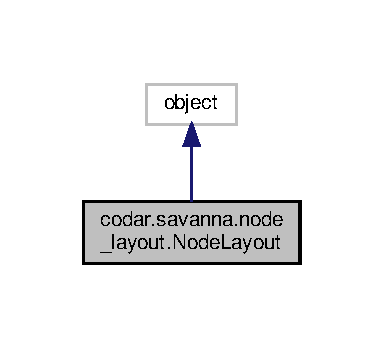
\includegraphics[width=184pt]{classcodar_1_1savanna_1_1node__layout_1_1_node_layout__inherit__graph}
\end{center}
\end{figure}


Collaboration diagram for codar.\+savanna.\+node\+\_\+layout.\+Node\+Layout\+:
\nopagebreak
\begin{figure}[H]
\begin{center}
\leavevmode
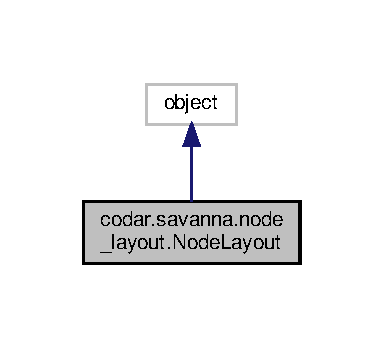
\includegraphics[width=184pt]{classcodar_1_1savanna_1_1node__layout_1_1_node_layout__coll__graph}
\end{center}
\end{figure}
\subsection*{Public Member Functions}
\begin{DoxyCompactItemize}
\item 
def \hyperlink{classcodar_1_1savanna_1_1node__layout_1_1_node_layout_af898ee59a1a5f520328a53d3b60a62d0}{\+\_\+\+\_\+init\+\_\+\+\_\+} (self, \hyperlink{classcodar_1_1savanna_1_1node__layout_1_1_node_layout_af27f209b198b9491d57d2bb3e65abc34}{layout\+\_\+list})
\item 
def \hyperlink{classcodar_1_1savanna_1_1node__layout_1_1_node_layout_ab0b94ca4a741efab71db5a598a782c38}{add\+\_\+node} (self, node\+\_\+dict)
\item 
def \hyperlink{classcodar_1_1savanna_1_1node__layout_1_1_node_layout_ae63a2f3c26294b78b35af77af4063899}{get\+\_\+node\+\_\+containing\+\_\+code} (self, code)
\item 
def \hyperlink{classcodar_1_1savanna_1_1node__layout_1_1_node_layout_add6c0879f2b8995f83cf07aaa09b7bbf}{codes\+\_\+per\+\_\+node} (self)
\item 
def \hyperlink{classcodar_1_1savanna_1_1node__layout_1_1_node_layout_a90f88aa1b664e9e9ed2b69e898c4581a}{shared\+\_\+nodes} (self)
\item 
def \hyperlink{classcodar_1_1savanna_1_1node__layout_1_1_node_layout_aa6d5b7f3721c264b0eeb3f7e7351c658}{ppn} (self)
\item 
def \hyperlink{classcodar_1_1savanna_1_1node__layout_1_1_node_layout_a9b1ef6ea6e08f60a04891db7ee460990}{validate} (self, \hyperlink{classcodar_1_1savanna_1_1node__layout_1_1_node_layout_aa6d5b7f3721c264b0eeb3f7e7351c658}{ppn}, \hyperlink{classcodar_1_1savanna_1_1node__layout_1_1_node_layout_add6c0879f2b8995f83cf07aaa09b7bbf}{codes\+\_\+per\+\_\+node}, \hyperlink{classcodar_1_1savanna_1_1node__layout_1_1_node_layout_a90f88aa1b664e9e9ed2b69e898c4581a}{shared\+\_\+nodes})
\item 
def \hyperlink{classcodar_1_1savanna_1_1node__layout_1_1_node_layout_ac75f6e66031d9e5c2f47ac0450335536}{as\+\_\+data\+\_\+list} (self)
\item 
def \hyperlink{classcodar_1_1savanna_1_1node__layout_1_1_node_layout_ae830687f476fdcc4036f141f3caad48b}{serialize\+\_\+to\+\_\+dict} (self)
\item 
def \hyperlink{classcodar_1_1savanna_1_1node__layout_1_1_node_layout_aa3b19766879e91de1698bb47d7149809}{copy} (self)
\item 
def \hyperlink{classcodar_1_1savanna_1_1node__layout_1_1_node_layout_a3f6f326ba64b563322c2b745775ab82b}{group\+\_\+codes\+\_\+by\+\_\+node} (self)
\item 
def \hyperlink{classcodar_1_1savanna_1_1node__layout_1_1_node_layout_addd066236434ca6fb9813fc50bcac973}{populate\+\_\+remaining} (self, rc\+\_\+names, \hyperlink{classcodar_1_1savanna_1_1node__layout_1_1_node_layout_aa6d5b7f3721c264b0eeb3f7e7351c658}{ppn})
\item 
def \hyperlink{classcodar_1_1savanna_1_1node__layout_1_1_node_layout_afa3112f3e4b98a1ad6f1c834dd81b2d7}{default\+\_\+no\+\_\+share\+\_\+layout} (cls, \hyperlink{classcodar_1_1savanna_1_1node__layout_1_1_node_layout_aa6d5b7f3721c264b0eeb3f7e7351c658}{ppn}, code\+\_\+names)
\end{DoxyCompactItemize}
\subsection*{Public Attributes}
\begin{DoxyCompactItemize}
\item 
\hyperlink{classcodar_1_1savanna_1_1node__layout_1_1_node_layout_af27f209b198b9491d57d2bb3e65abc34}{layout\+\_\+list}
\item 
\hyperlink{classcodar_1_1savanna_1_1node__layout_1_1_node_layout_a4bda626f4487b5078f83744cf7d32b7d}{layout\+\_\+map}
\end{DoxyCompactItemize}


\subsection{Detailed Description}
\begin{DoxyVerb}Class representing options on how to organize a multi-exe task across
many nodes. It is the scheduler model's job to take this and produce the
correct scheduler and runner options to make this happen, or raise an error
if it's not possible. Note that this will generally be different for each
machine unless it is very simple and suppored uniformly by all desired
machines.

A layout is represented as a list of dictionaries, where each dictionary
described codes to be run together on a single node. The keys are
the names of the codes, and the values are the number of processes to
assign to each.
\end{DoxyVerb}
 

Definition at line 6 of file node\+\_\+layout.\+py.



\subsection{Constructor \& Destructor Documentation}
\mbox{\Hypertarget{classcodar_1_1savanna_1_1node__layout_1_1_node_layout_af898ee59a1a5f520328a53d3b60a62d0}\label{classcodar_1_1savanna_1_1node__layout_1_1_node_layout_af898ee59a1a5f520328a53d3b60a62d0}} 
\index{codar\+::savanna\+::node\+\_\+layout\+::\+Node\+Layout@{codar\+::savanna\+::node\+\_\+layout\+::\+Node\+Layout}!\+\_\+\+\_\+init\+\_\+\+\_\+@{\+\_\+\+\_\+init\+\_\+\+\_\+}}
\index{\+\_\+\+\_\+init\+\_\+\+\_\+@{\+\_\+\+\_\+init\+\_\+\+\_\+}!codar\+::savanna\+::node\+\_\+layout\+::\+Node\+Layout@{codar\+::savanna\+::node\+\_\+layout\+::\+Node\+Layout}}
\subsubsection{\texorpdfstring{\+\_\+\+\_\+init\+\_\+\+\_\+()}{\_\_init\_\_()}}
{\footnotesize\ttfamily def codar.\+savanna.\+node\+\_\+layout.\+Node\+Layout.\+\_\+\+\_\+init\+\_\+\+\_\+ (\begin{DoxyParamCaption}\item[{}]{self,  }\item[{}]{layout\+\_\+list }\end{DoxyParamCaption})}



Definition at line 20 of file node\+\_\+layout.\+py.



\subsection{Member Function Documentation}
\mbox{\Hypertarget{classcodar_1_1savanna_1_1node__layout_1_1_node_layout_ab0b94ca4a741efab71db5a598a782c38}\label{classcodar_1_1savanna_1_1node__layout_1_1_node_layout_ab0b94ca4a741efab71db5a598a782c38}} 
\index{codar\+::savanna\+::node\+\_\+layout\+::\+Node\+Layout@{codar\+::savanna\+::node\+\_\+layout\+::\+Node\+Layout}!add\+\_\+node@{add\+\_\+node}}
\index{add\+\_\+node@{add\+\_\+node}!codar\+::savanna\+::node\+\_\+layout\+::\+Node\+Layout@{codar\+::savanna\+::node\+\_\+layout\+::\+Node\+Layout}}
\subsubsection{\texorpdfstring{add\+\_\+node()}{add\_node()}}
{\footnotesize\ttfamily def codar.\+savanna.\+node\+\_\+layout.\+Node\+Layout.\+add\+\_\+node (\begin{DoxyParamCaption}\item[{}]{self,  }\item[{}]{node\+\_\+dict }\end{DoxyParamCaption})}

\begin{DoxyVerb}Add a node to an existing layout, e.g. add sosflow.\end{DoxyVerb}
 

Definition at line 43 of file node\+\_\+layout.\+py.

\mbox{\Hypertarget{classcodar_1_1savanna_1_1node__layout_1_1_node_layout_ac75f6e66031d9e5c2f47ac0450335536}\label{classcodar_1_1savanna_1_1node__layout_1_1_node_layout_ac75f6e66031d9e5c2f47ac0450335536}} 
\index{codar\+::savanna\+::node\+\_\+layout\+::\+Node\+Layout@{codar\+::savanna\+::node\+\_\+layout\+::\+Node\+Layout}!as\+\_\+data\+\_\+list@{as\+\_\+data\+\_\+list}}
\index{as\+\_\+data\+\_\+list@{as\+\_\+data\+\_\+list}!codar\+::savanna\+::node\+\_\+layout\+::\+Node\+Layout@{codar\+::savanna\+::node\+\_\+layout\+::\+Node\+Layout}}
\subsubsection{\texorpdfstring{as\+\_\+data\+\_\+list()}{as\_data\_list()}}
{\footnotesize\ttfamily def codar.\+savanna.\+node\+\_\+layout.\+Node\+Layout.\+as\+\_\+data\+\_\+list (\begin{DoxyParamCaption}\item[{}]{self }\end{DoxyParamCaption})}



Definition at line 114 of file node\+\_\+layout.\+py.

\mbox{\Hypertarget{classcodar_1_1savanna_1_1node__layout_1_1_node_layout_add6c0879f2b8995f83cf07aaa09b7bbf}\label{classcodar_1_1savanna_1_1node__layout_1_1_node_layout_add6c0879f2b8995f83cf07aaa09b7bbf}} 
\index{codar\+::savanna\+::node\+\_\+layout\+::\+Node\+Layout@{codar\+::savanna\+::node\+\_\+layout\+::\+Node\+Layout}!codes\+\_\+per\+\_\+node@{codes\+\_\+per\+\_\+node}}
\index{codes\+\_\+per\+\_\+node@{codes\+\_\+per\+\_\+node}!codar\+::savanna\+::node\+\_\+layout\+::\+Node\+Layout@{codar\+::savanna\+::node\+\_\+layout\+::\+Node\+Layout}}
\subsubsection{\texorpdfstring{codes\+\_\+per\+\_\+node()}{codes\_per\_node()}}
{\footnotesize\ttfamily def codar.\+savanna.\+node\+\_\+layout.\+Node\+Layout.\+codes\+\_\+per\+\_\+node (\begin{DoxyParamCaption}\item[{}]{self }\end{DoxyParamCaption})}



Definition at line 55 of file node\+\_\+layout.\+py.

\mbox{\Hypertarget{classcodar_1_1savanna_1_1node__layout_1_1_node_layout_aa3b19766879e91de1698bb47d7149809}\label{classcodar_1_1savanna_1_1node__layout_1_1_node_layout_aa3b19766879e91de1698bb47d7149809}} 
\index{codar\+::savanna\+::node\+\_\+layout\+::\+Node\+Layout@{codar\+::savanna\+::node\+\_\+layout\+::\+Node\+Layout}!copy@{copy}}
\index{copy@{copy}!codar\+::savanna\+::node\+\_\+layout\+::\+Node\+Layout@{codar\+::savanna\+::node\+\_\+layout\+::\+Node\+Layout}}
\subsubsection{\texorpdfstring{copy()}{copy()}}
{\footnotesize\ttfamily def codar.\+savanna.\+node\+\_\+layout.\+Node\+Layout.\+copy (\begin{DoxyParamCaption}\item[{}]{self }\end{DoxyParamCaption})}



Definition at line 129 of file node\+\_\+layout.\+py.

\mbox{\Hypertarget{classcodar_1_1savanna_1_1node__layout_1_1_node_layout_afa3112f3e4b98a1ad6f1c834dd81b2d7}\label{classcodar_1_1savanna_1_1node__layout_1_1_node_layout_afa3112f3e4b98a1ad6f1c834dd81b2d7}} 
\index{codar\+::savanna\+::node\+\_\+layout\+::\+Node\+Layout@{codar\+::savanna\+::node\+\_\+layout\+::\+Node\+Layout}!default\+\_\+no\+\_\+share\+\_\+layout@{default\+\_\+no\+\_\+share\+\_\+layout}}
\index{default\+\_\+no\+\_\+share\+\_\+layout@{default\+\_\+no\+\_\+share\+\_\+layout}!codar\+::savanna\+::node\+\_\+layout\+::\+Node\+Layout@{codar\+::savanna\+::node\+\_\+layout\+::\+Node\+Layout}}
\subsubsection{\texorpdfstring{default\+\_\+no\+\_\+share\+\_\+layout()}{default\_no\_share\_layout()}}
{\footnotesize\ttfamily def codar.\+savanna.\+node\+\_\+layout.\+Node\+Layout.\+default\+\_\+no\+\_\+share\+\_\+layout (\begin{DoxyParamCaption}\item[{}]{cls,  }\item[{}]{ppn,  }\item[{}]{code\+\_\+names }\end{DoxyParamCaption})}

\begin{DoxyVerb}Create a layout object for the specified codes and ppn, where each
code uses max procs on it's own node.\end{DoxyVerb}
 

Definition at line 173 of file node\+\_\+layout.\+py.

\mbox{\Hypertarget{classcodar_1_1savanna_1_1node__layout_1_1_node_layout_ae63a2f3c26294b78b35af77af4063899}\label{classcodar_1_1savanna_1_1node__layout_1_1_node_layout_ae63a2f3c26294b78b35af77af4063899}} 
\index{codar\+::savanna\+::node\+\_\+layout\+::\+Node\+Layout@{codar\+::savanna\+::node\+\_\+layout\+::\+Node\+Layout}!get\+\_\+node\+\_\+containing\+\_\+code@{get\+\_\+node\+\_\+containing\+\_\+code}}
\index{get\+\_\+node\+\_\+containing\+\_\+code@{get\+\_\+node\+\_\+containing\+\_\+code}!codar\+::savanna\+::node\+\_\+layout\+::\+Node\+Layout@{codar\+::savanna\+::node\+\_\+layout\+::\+Node\+Layout}}
\subsubsection{\texorpdfstring{get\+\_\+node\+\_\+containing\+\_\+code()}{get\_node\_containing\_code()}}
{\footnotesize\ttfamily def codar.\+savanna.\+node\+\_\+layout.\+Node\+Layout.\+get\+\_\+node\+\_\+containing\+\_\+code (\begin{DoxyParamCaption}\item[{}]{self,  }\item[{}]{code }\end{DoxyParamCaption})}

\begin{DoxyVerb}Get node dict containing the specified code. Raises KeyError if
not found.\end{DoxyVerb}
 

Definition at line 50 of file node\+\_\+layout.\+py.

\mbox{\Hypertarget{classcodar_1_1savanna_1_1node__layout_1_1_node_layout_a3f6f326ba64b563322c2b745775ab82b}\label{classcodar_1_1savanna_1_1node__layout_1_1_node_layout_a3f6f326ba64b563322c2b745775ab82b}} 
\index{codar\+::savanna\+::node\+\_\+layout\+::\+Node\+Layout@{codar\+::savanna\+::node\+\_\+layout\+::\+Node\+Layout}!group\+\_\+codes\+\_\+by\+\_\+node@{group\+\_\+codes\+\_\+by\+\_\+node}}
\index{group\+\_\+codes\+\_\+by\+\_\+node@{group\+\_\+codes\+\_\+by\+\_\+node}!codar\+::savanna\+::node\+\_\+layout\+::\+Node\+Layout@{codar\+::savanna\+::node\+\_\+layout\+::\+Node\+Layout}}
\subsubsection{\texorpdfstring{group\+\_\+codes\+\_\+by\+\_\+node()}{group\_codes\_by\_node()}}
{\footnotesize\ttfamily def codar.\+savanna.\+node\+\_\+layout.\+Node\+Layout.\+group\+\_\+codes\+\_\+by\+\_\+node (\begin{DoxyParamCaption}\item[{}]{self }\end{DoxyParamCaption})}

\begin{DoxyVerb}Return a list of dicts, where each list represents codes on a
node, and a dict key for ppn
Example: [ {sim,analysis1}, {analysis2}, {viz} ].
Must take Summit NodeConfigs into account\end{DoxyVerb}
 

Definition at line 132 of file node\+\_\+layout.\+py.

\mbox{\Hypertarget{classcodar_1_1savanna_1_1node__layout_1_1_node_layout_addd066236434ca6fb9813fc50bcac973}\label{classcodar_1_1savanna_1_1node__layout_1_1_node_layout_addd066236434ca6fb9813fc50bcac973}} 
\index{codar\+::savanna\+::node\+\_\+layout\+::\+Node\+Layout@{codar\+::savanna\+::node\+\_\+layout\+::\+Node\+Layout}!populate\+\_\+remaining@{populate\+\_\+remaining}}
\index{populate\+\_\+remaining@{populate\+\_\+remaining}!codar\+::savanna\+::node\+\_\+layout\+::\+Node\+Layout@{codar\+::savanna\+::node\+\_\+layout\+::\+Node\+Layout}}
\subsubsection{\texorpdfstring{populate\+\_\+remaining()}{populate\_remaining()}}
{\footnotesize\ttfamily def codar.\+savanna.\+node\+\_\+layout.\+Node\+Layout.\+populate\+\_\+remaining (\begin{DoxyParamCaption}\item[{}]{self,  }\item[{}]{rc\+\_\+names,  }\item[{}]{ppn }\end{DoxyParamCaption})}



Definition at line 161 of file node\+\_\+layout.\+py.

\mbox{\Hypertarget{classcodar_1_1savanna_1_1node__layout_1_1_node_layout_aa6d5b7f3721c264b0eeb3f7e7351c658}\label{classcodar_1_1savanna_1_1node__layout_1_1_node_layout_aa6d5b7f3721c264b0eeb3f7e7351c658}} 
\index{codar\+::savanna\+::node\+\_\+layout\+::\+Node\+Layout@{codar\+::savanna\+::node\+\_\+layout\+::\+Node\+Layout}!ppn@{ppn}}
\index{ppn@{ppn}!codar\+::savanna\+::node\+\_\+layout\+::\+Node\+Layout@{codar\+::savanna\+::node\+\_\+layout\+::\+Node\+Layout}}
\subsubsection{\texorpdfstring{ppn()}{ppn()}}
{\footnotesize\ttfamily def codar.\+savanna.\+node\+\_\+layout.\+Node\+Layout.\+ppn (\begin{DoxyParamCaption}\item[{}]{self }\end{DoxyParamCaption})}



Definition at line 61 of file node\+\_\+layout.\+py.

\mbox{\Hypertarget{classcodar_1_1savanna_1_1node__layout_1_1_node_layout_ae830687f476fdcc4036f141f3caad48b}\label{classcodar_1_1savanna_1_1node__layout_1_1_node_layout_ae830687f476fdcc4036f141f3caad48b}} 
\index{codar\+::savanna\+::node\+\_\+layout\+::\+Node\+Layout@{codar\+::savanna\+::node\+\_\+layout\+::\+Node\+Layout}!serialize\+\_\+to\+\_\+dict@{serialize\+\_\+to\+\_\+dict}}
\index{serialize\+\_\+to\+\_\+dict@{serialize\+\_\+to\+\_\+dict}!codar\+::savanna\+::node\+\_\+layout\+::\+Node\+Layout@{codar\+::savanna\+::node\+\_\+layout\+::\+Node\+Layout}}
\subsubsection{\texorpdfstring{serialize\+\_\+to\+\_\+dict()}{serialize\_to\_dict()}}
{\footnotesize\ttfamily def codar.\+savanna.\+node\+\_\+layout.\+Node\+Layout.\+serialize\+\_\+to\+\_\+dict (\begin{DoxyParamCaption}\item[{}]{self }\end{DoxyParamCaption})}

\begin{DoxyVerb}Get a copy of the data list passed to the constructor,
suitable for JSON serialization.\end{DoxyVerb}
 

Definition at line 117 of file node\+\_\+layout.\+py.

\mbox{\Hypertarget{classcodar_1_1savanna_1_1node__layout_1_1_node_layout_a90f88aa1b664e9e9ed2b69e898c4581a}\label{classcodar_1_1savanna_1_1node__layout_1_1_node_layout_a90f88aa1b664e9e9ed2b69e898c4581a}} 
\index{codar\+::savanna\+::node\+\_\+layout\+::\+Node\+Layout@{codar\+::savanna\+::node\+\_\+layout\+::\+Node\+Layout}!shared\+\_\+nodes@{shared\+\_\+nodes}}
\index{shared\+\_\+nodes@{shared\+\_\+nodes}!codar\+::savanna\+::node\+\_\+layout\+::\+Node\+Layout@{codar\+::savanna\+::node\+\_\+layout\+::\+Node\+Layout}}
\subsubsection{\texorpdfstring{shared\+\_\+nodes()}{shared\_nodes()}}
{\footnotesize\ttfamily def codar.\+savanna.\+node\+\_\+layout.\+Node\+Layout.\+shared\+\_\+nodes (\begin{DoxyParamCaption}\item[{}]{self }\end{DoxyParamCaption})}



Definition at line 58 of file node\+\_\+layout.\+py.

\mbox{\Hypertarget{classcodar_1_1savanna_1_1node__layout_1_1_node_layout_a9b1ef6ea6e08f60a04891db7ee460990}\label{classcodar_1_1savanna_1_1node__layout_1_1_node_layout_a9b1ef6ea6e08f60a04891db7ee460990}} 
\index{codar\+::savanna\+::node\+\_\+layout\+::\+Node\+Layout@{codar\+::savanna\+::node\+\_\+layout\+::\+Node\+Layout}!validate@{validate}}
\index{validate@{validate}!codar\+::savanna\+::node\+\_\+layout\+::\+Node\+Layout@{codar\+::savanna\+::node\+\_\+layout\+::\+Node\+Layout}}
\subsubsection{\texorpdfstring{validate()}{validate()}}
{\footnotesize\ttfamily def codar.\+savanna.\+node\+\_\+layout.\+Node\+Layout.\+validate (\begin{DoxyParamCaption}\item[{}]{self,  }\item[{}]{ppn,  }\item[{}]{codes\+\_\+per\+\_\+node,  }\item[{}]{shared\+\_\+nodes }\end{DoxyParamCaption})}

\begin{DoxyVerb}Given a machine ppn and max numer of codes (e.g. 4 on cori),
raise a ValueError if the specified layout won't fit.
Dont modify this yet, this is being used by the tests\end{DoxyVerb}
 

Definition at line 96 of file node\+\_\+layout.\+py.



\subsection{Member Data Documentation}
\mbox{\Hypertarget{classcodar_1_1savanna_1_1node__layout_1_1_node_layout_af27f209b198b9491d57d2bb3e65abc34}\label{classcodar_1_1savanna_1_1node__layout_1_1_node_layout_af27f209b198b9491d57d2bb3e65abc34}} 
\index{codar\+::savanna\+::node\+\_\+layout\+::\+Node\+Layout@{codar\+::savanna\+::node\+\_\+layout\+::\+Node\+Layout}!layout\+\_\+list@{layout\+\_\+list}}
\index{layout\+\_\+list@{layout\+\_\+list}!codar\+::savanna\+::node\+\_\+layout\+::\+Node\+Layout@{codar\+::savanna\+::node\+\_\+layout\+::\+Node\+Layout}}
\subsubsection{\texorpdfstring{layout\+\_\+list}{layout\_list}}
{\footnotesize\ttfamily codar.\+savanna.\+node\+\_\+layout.\+Node\+Layout.\+layout\+\_\+list}



Definition at line 34 of file node\+\_\+layout.\+py.

\mbox{\Hypertarget{classcodar_1_1savanna_1_1node__layout_1_1_node_layout_a4bda626f4487b5078f83744cf7d32b7d}\label{classcodar_1_1savanna_1_1node__layout_1_1_node_layout_a4bda626f4487b5078f83744cf7d32b7d}} 
\index{codar\+::savanna\+::node\+\_\+layout\+::\+Node\+Layout@{codar\+::savanna\+::node\+\_\+layout\+::\+Node\+Layout}!layout\+\_\+map@{layout\+\_\+map}}
\index{layout\+\_\+map@{layout\+\_\+map}!codar\+::savanna\+::node\+\_\+layout\+::\+Node\+Layout@{codar\+::savanna\+::node\+\_\+layout\+::\+Node\+Layout}}
\subsubsection{\texorpdfstring{layout\+\_\+map}{layout\_map}}
{\footnotesize\ttfamily codar.\+savanna.\+node\+\_\+layout.\+Node\+Layout.\+layout\+\_\+map}



Definition at line 35 of file node\+\_\+layout.\+py.



The documentation for this class was generated from the following file\+:\begin{DoxyCompactItemize}
\item 
\hyperlink{node__layout_8py}{node\+\_\+layout.\+py}\end{DoxyCompactItemize}

\hypertarget{classcodar_1_1savanna_1_1model_1_1_pipeline}{}\section{codar.\+savanna.\+model.\+Pipeline Class Reference}
\label{classcodar_1_1savanna_1_1model_1_1_pipeline}\index{codar.\+savanna.\+model.\+Pipeline@{codar.\+savanna.\+model.\+Pipeline}}


Inheritance diagram for codar.\+savanna.\+model.\+Pipeline\+:
\nopagebreak
\begin{figure}[H]
\begin{center}
\leavevmode
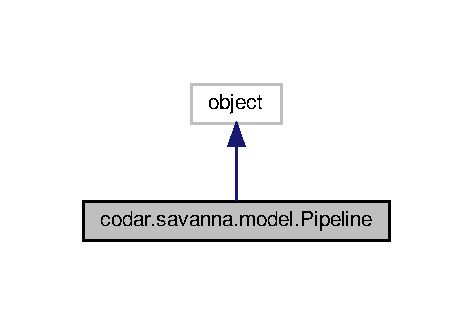
\includegraphics[width=227pt]{classcodar_1_1savanna_1_1model_1_1_pipeline__inherit__graph}
\end{center}
\end{figure}


Collaboration diagram for codar.\+savanna.\+model.\+Pipeline\+:
\nopagebreak
\begin{figure}[H]
\begin{center}
\leavevmode
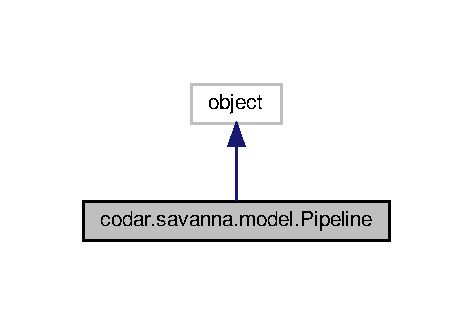
\includegraphics[width=227pt]{classcodar_1_1savanna_1_1model_1_1_pipeline__coll__graph}
\end{center}
\end{figure}
\subsection*{Public Member Functions}
\begin{DoxyCompactItemize}
\item 
def \hyperlink{classcodar_1_1savanna_1_1model_1_1_pipeline_ada8df2357966f7e3cc7c34d3ee36f9a1}{\+\_\+\+\_\+init\+\_\+\+\_\+} (self, pipe\+\_\+id, \hyperlink{classcodar_1_1savanna_1_1model_1_1_pipeline_aceeec7aae018e27934619f797162d458}{runs}, \hyperlink{classcodar_1_1savanna_1_1model_1_1_pipeline_a2272c691cd2ecb1b11b581341cd5707c}{working\+\_\+dir}, \hyperlink{classcodar_1_1savanna_1_1model_1_1_pipeline_ae5ea9a86523bdbbc9537a37b6d01436c}{total\+\_\+nodes}, \hyperlink{classcodar_1_1savanna_1_1model_1_1_pipeline_a7492ac83160febb20e9a60dad2a9233f}{machine\+\_\+name}, \hyperlink{classcodar_1_1savanna_1_1model_1_1_pipeline_a8f831647499af6eae5696a85abc9a449}{kill\+\_\+on\+\_\+partial\+\_\+failure}=False, \hyperlink{classcodar_1_1savanna_1_1model_1_1_pipeline_a5539114ad7bace8f9753064e3d4a28ec}{post\+\_\+process\+\_\+script}=None, \hyperlink{classcodar_1_1savanna_1_1model_1_1_pipeline_a4568a89046b0fc45c5e6f3f5d80588a1}{post\+\_\+process\+\_\+args}=None, \hyperlink{classcodar_1_1savanna_1_1model_1_1_pipeline_aed4a93e26e62b1878c277a6d9a992fa9}{post\+\_\+process\+\_\+stop\+\_\+on\+\_\+failure}=False, \hyperlink{classcodar_1_1savanna_1_1model_1_1_pipeline_a32c1000ef2bf29a77c0f7ca8849adb64}{node\+\_\+layout}=None, \hyperlink{classcodar_1_1savanna_1_1model_1_1_pipeline_a93c4ea2d9b1714d9f78aba21c1507e95}{launch\+\_\+mode}=None)
\item 
def \hyperlink{classcodar_1_1savanna_1_1model_1_1_pipeline_abf71facf9275710199941f0f79997db2}{from\+\_\+data} (cls, data)
\item 
def \hyperlink{classcodar_1_1savanna_1_1model_1_1_pipeline_ad7ddded563710c1a240b850c56a3fd3c}{start} (self, consumer, \hyperlink{classcodar_1_1savanna_1_1model_1_1_pipeline_ae821850c02f50972fa0edb2284ff9c59}{nodes\+\_\+assigned}, runner=None)
\item 
def \hyperlink{classcodar_1_1savanna_1_1model_1_1_pipeline_a0a7fe2d4e57a5604ae9d997caeee2f87}{run\+\_\+finished} (self, run)
\item 
def \hyperlink{classcodar_1_1savanna_1_1model_1_1_pipeline_a9a21933f3cc3457a161029b4f708997b}{run\+\_\+post\+\_\+process\+\_\+script} (self)
\item 
def \hyperlink{classcodar_1_1savanna_1_1model_1_1_pipeline_a05bcb6afe339fb967d8d358d5c6037ca}{add\+\_\+done\+\_\+callback} (self, fn)
\item 
def \hyperlink{classcodar_1_1savanna_1_1model_1_1_pipeline_aa1656c8b4ec886ef96521dfb137c123b}{remove\+\_\+done\+\_\+callback} (self, fn)
\item 
def \hyperlink{classcodar_1_1savanna_1_1model_1_1_pipeline_ac13dbe4331eff67d4306a11a06199e3e}{add\+\_\+fatal\+\_\+callback} (self, fn)
\item 
def \hyperlink{classcodar_1_1savanna_1_1model_1_1_pipeline_a6ddff7f98a8fd2aa7066343540c8bab0}{remove\+\_\+fatal\+\_\+callback} (self, fn)
\item 
def \hyperlink{classcodar_1_1savanna_1_1model_1_1_pipeline_a0c85356d538d06651c7ed18ceb7c1ce5}{get\+\_\+nodes\+\_\+used} (self)
\item 
def \hyperlink{classcodar_1_1savanna_1_1model_1_1_pipeline_a559b6f3f07dc06fd1c42a33fff9e96f1}{set\+\_\+ppn} (self, ppn)
\item 
def \hyperlink{classcodar_1_1savanna_1_1model_1_1_pipeline_a372fa98a663eccfd0c629e9e92f411f8}{set\+\_\+total\+\_\+nodes} (self)
\item 
def \hyperlink{classcodar_1_1savanna_1_1model_1_1_pipeline_a415914cbdd84133196a9f4c612be5313}{get\+\_\+state} (self)
\item 
def \hyperlink{classcodar_1_1savanna_1_1model_1_1_pipeline_a45f720376f4a44a4d87777c572c7dd3c}{get\+\_\+pids} (self)
\item 
def \hyperlink{classcodar_1_1savanna_1_1model_1_1_pipeline_accc64a044c6e1929d19cbea5718fd0f7}{force\+\_\+kill\+\_\+all} (self)
\item 
def \hyperlink{classcodar_1_1savanna_1_1model_1_1_pipeline_a663e76af6faf61c9791dfc925786a859}{join\+\_\+all} (self)
\end{DoxyCompactItemize}
\subsection*{Public Attributes}
\begin{DoxyCompactItemize}
\item 
\hyperlink{classcodar_1_1savanna_1_1model_1_1_pipeline_ac9d67caac17820b586b007df1411e3f8}{id}
\item 
\hyperlink{classcodar_1_1savanna_1_1model_1_1_pipeline_aceeec7aae018e27934619f797162d458}{runs}
\item 
\hyperlink{classcodar_1_1savanna_1_1model_1_1_pipeline_a2272c691cd2ecb1b11b581341cd5707c}{working\+\_\+dir}
\item 
\hyperlink{classcodar_1_1savanna_1_1model_1_1_pipeline_a8f831647499af6eae5696a85abc9a449}{kill\+\_\+on\+\_\+partial\+\_\+failure}
\item 
\hyperlink{classcodar_1_1savanna_1_1model_1_1_pipeline_a5539114ad7bace8f9753064e3d4a28ec}{post\+\_\+process\+\_\+script}
\item 
\hyperlink{classcodar_1_1savanna_1_1model_1_1_pipeline_a4568a89046b0fc45c5e6f3f5d80588a1}{post\+\_\+process\+\_\+args}
\item 
\hyperlink{classcodar_1_1savanna_1_1model_1_1_pipeline_aed4a93e26e62b1878c277a6d9a992fa9}{post\+\_\+process\+\_\+stop\+\_\+on\+\_\+failure}
\item 
\hyperlink{classcodar_1_1savanna_1_1model_1_1_pipeline_a32c1000ef2bf29a77c0f7ca8849adb64}{node\+\_\+layout}
\item 
\hyperlink{classcodar_1_1savanna_1_1model_1_1_pipeline_a7492ac83160febb20e9a60dad2a9233f}{machine\+\_\+name}
\item 
\hyperlink{classcodar_1_1savanna_1_1model_1_1_pipeline_a10bd363eae4d4b4e00c86fe26c2adedf}{done\+\_\+callbacks}
\item 
\hyperlink{classcodar_1_1savanna_1_1model_1_1_pipeline_a86657c62c6922840292d1f11e455016b}{fatal\+\_\+callbacks}
\item 
\hyperlink{classcodar_1_1savanna_1_1model_1_1_pipeline_a87f9ace8a7b25f52efa9e63821b8ea87}{total\+\_\+procs}
\item 
\hyperlink{classcodar_1_1savanna_1_1model_1_1_pipeline_a461a521150825c07864b23ff66c7cd69}{log\+\_\+prefix}
\item 
\hyperlink{classcodar_1_1savanna_1_1model_1_1_pipeline_ae5ea9a86523bdbbc9537a37b6d01436c}{total\+\_\+nodes}
\item 
\hyperlink{classcodar_1_1savanna_1_1model_1_1_pipeline_a93c4ea2d9b1714d9f78aba21c1507e95}{launch\+\_\+mode}
\item 
\hyperlink{classcodar_1_1savanna_1_1model_1_1_pipeline_ae821850c02f50972fa0edb2284ff9c59}{nodes\+\_\+assigned}
\end{DoxyCompactItemize}


\subsection{Detailed Description}


Definition at line 449 of file model.\+py.



\subsection{Constructor \& Destructor Documentation}
\mbox{\Hypertarget{classcodar_1_1savanna_1_1model_1_1_pipeline_ada8df2357966f7e3cc7c34d3ee36f9a1}\label{classcodar_1_1savanna_1_1model_1_1_pipeline_ada8df2357966f7e3cc7c34d3ee36f9a1}} 
\index{codar\+::savanna\+::model\+::\+Pipeline@{codar\+::savanna\+::model\+::\+Pipeline}!\+\_\+\+\_\+init\+\_\+\+\_\+@{\+\_\+\+\_\+init\+\_\+\+\_\+}}
\index{\+\_\+\+\_\+init\+\_\+\+\_\+@{\+\_\+\+\_\+init\+\_\+\+\_\+}!codar\+::savanna\+::model\+::\+Pipeline@{codar\+::savanna\+::model\+::\+Pipeline}}
\subsubsection{\texorpdfstring{\+\_\+\+\_\+init\+\_\+\+\_\+()}{\_\_init\_\_()}}
{\footnotesize\ttfamily def codar.\+savanna.\+model.\+Pipeline.\+\_\+\+\_\+init\+\_\+\+\_\+ (\begin{DoxyParamCaption}\item[{}]{self,  }\item[{}]{pipe\+\_\+id,  }\item[{}]{runs,  }\item[{}]{working\+\_\+dir,  }\item[{}]{total\+\_\+nodes,  }\item[{}]{machine\+\_\+name,  }\item[{}]{kill\+\_\+on\+\_\+partial\+\_\+failure = {\ttfamily False},  }\item[{}]{post\+\_\+process\+\_\+script = {\ttfamily None},  }\item[{}]{post\+\_\+process\+\_\+args = {\ttfamily None},  }\item[{}]{post\+\_\+process\+\_\+stop\+\_\+on\+\_\+failure = {\ttfamily False},  }\item[{}]{node\+\_\+layout = {\ttfamily None},  }\item[{}]{launch\+\_\+mode = {\ttfamily None} }\end{DoxyParamCaption})}



Definition at line 455 of file model.\+py.



\subsection{Member Function Documentation}
\mbox{\Hypertarget{classcodar_1_1savanna_1_1model_1_1_pipeline_a05bcb6afe339fb967d8d358d5c6037ca}\label{classcodar_1_1savanna_1_1model_1_1_pipeline_a05bcb6afe339fb967d8d358d5c6037ca}} 
\index{codar\+::savanna\+::model\+::\+Pipeline@{codar\+::savanna\+::model\+::\+Pipeline}!add\+\_\+done\+\_\+callback@{add\+\_\+done\+\_\+callback}}
\index{add\+\_\+done\+\_\+callback@{add\+\_\+done\+\_\+callback}!codar\+::savanna\+::model\+::\+Pipeline@{codar\+::savanna\+::model\+::\+Pipeline}}
\subsubsection{\texorpdfstring{add\+\_\+done\+\_\+callback()}{add\_done\_callback()}}
{\footnotesize\ttfamily def codar.\+savanna.\+model.\+Pipeline.\+add\+\_\+done\+\_\+callback (\begin{DoxyParamCaption}\item[{}]{self,  }\item[{}]{fn }\end{DoxyParamCaption})}



Definition at line 818 of file model.\+py.

\mbox{\Hypertarget{classcodar_1_1savanna_1_1model_1_1_pipeline_ac13dbe4331eff67d4306a11a06199e3e}\label{classcodar_1_1savanna_1_1model_1_1_pipeline_ac13dbe4331eff67d4306a11a06199e3e}} 
\index{codar\+::savanna\+::model\+::\+Pipeline@{codar\+::savanna\+::model\+::\+Pipeline}!add\+\_\+fatal\+\_\+callback@{add\+\_\+fatal\+\_\+callback}}
\index{add\+\_\+fatal\+\_\+callback@{add\+\_\+fatal\+\_\+callback}!codar\+::savanna\+::model\+::\+Pipeline@{codar\+::savanna\+::model\+::\+Pipeline}}
\subsubsection{\texorpdfstring{add\+\_\+fatal\+\_\+callback()}{add\_fatal\_callback()}}
{\footnotesize\ttfamily def codar.\+savanna.\+model.\+Pipeline.\+add\+\_\+fatal\+\_\+callback (\begin{DoxyParamCaption}\item[{}]{self,  }\item[{}]{fn }\end{DoxyParamCaption})}



Definition at line 830 of file model.\+py.

\mbox{\Hypertarget{classcodar_1_1savanna_1_1model_1_1_pipeline_accc64a044c6e1929d19cbea5718fd0f7}\label{classcodar_1_1savanna_1_1model_1_1_pipeline_accc64a044c6e1929d19cbea5718fd0f7}} 
\index{codar\+::savanna\+::model\+::\+Pipeline@{codar\+::savanna\+::model\+::\+Pipeline}!force\+\_\+kill\+\_\+all@{force\+\_\+kill\+\_\+all}}
\index{force\+\_\+kill\+\_\+all@{force\+\_\+kill\+\_\+all}!codar\+::savanna\+::model\+::\+Pipeline@{codar\+::savanna\+::model\+::\+Pipeline}}
\subsubsection{\texorpdfstring{force\+\_\+kill\+\_\+all()}{force\_kill\_all()}}
{\footnotesize\ttfamily def codar.\+savanna.\+model.\+Pipeline.\+force\+\_\+kill\+\_\+all (\begin{DoxyParamCaption}\item[{}]{self }\end{DoxyParamCaption})}

\begin{DoxyVerb}Kill all runs and don't run post processing. Note that this call may
block waiting for all runs to be started, to avoid confusing races.
If the pipeline is already done, this does nothing. If one or more
runs are still active, or have not yet been marked as finished, then
it will mark the entire pipeline as killed so it can be re-run from
scratch on a restart if desired.
\end{DoxyVerb}
 

Definition at line 912 of file model.\+py.

\mbox{\Hypertarget{classcodar_1_1savanna_1_1model_1_1_pipeline_abf71facf9275710199941f0f79997db2}\label{classcodar_1_1savanna_1_1model_1_1_pipeline_abf71facf9275710199941f0f79997db2}} 
\index{codar\+::savanna\+::model\+::\+Pipeline@{codar\+::savanna\+::model\+::\+Pipeline}!from\+\_\+data@{from\+\_\+data}}
\index{from\+\_\+data@{from\+\_\+data}!codar\+::savanna\+::model\+::\+Pipeline@{codar\+::savanna\+::model\+::\+Pipeline}}
\subsubsection{\texorpdfstring{from\+\_\+data()}{from\_data()}}
{\footnotesize\ttfamily def codar.\+savanna.\+model.\+Pipeline.\+from\+\_\+data (\begin{DoxyParamCaption}\item[{}]{cls,  }\item[{}]{data }\end{DoxyParamCaption})}

\begin{DoxyVerb}Create Pipeline instance from dictionary data structure, containing
at least "id" and "runs" keys. The "runs" key must have a list of dict,
and each dict is parsed using Run.from_data.
Raises KeyError if a required key is missing.\end{DoxyVerb}
 

Definition at line 497 of file model.\+py.

\mbox{\Hypertarget{classcodar_1_1savanna_1_1model_1_1_pipeline_a0c85356d538d06651c7ed18ceb7c1ce5}\label{classcodar_1_1savanna_1_1model_1_1_pipeline_a0c85356d538d06651c7ed18ceb7c1ce5}} 
\index{codar\+::savanna\+::model\+::\+Pipeline@{codar\+::savanna\+::model\+::\+Pipeline}!get\+\_\+nodes\+\_\+used@{get\+\_\+nodes\+\_\+used}}
\index{get\+\_\+nodes\+\_\+used@{get\+\_\+nodes\+\_\+used}!codar\+::savanna\+::model\+::\+Pipeline@{codar\+::savanna\+::model\+::\+Pipeline}}
\subsubsection{\texorpdfstring{get\+\_\+nodes\+\_\+used()}{get\_nodes\_used()}}
{\footnotesize\ttfamily def codar.\+savanna.\+model.\+Pipeline.\+get\+\_\+nodes\+\_\+used (\begin{DoxyParamCaption}\item[{}]{self }\end{DoxyParamCaption})}



Definition at line 850 of file model.\+py.

\mbox{\Hypertarget{classcodar_1_1savanna_1_1model_1_1_pipeline_a45f720376f4a44a4d87777c572c7dd3c}\label{classcodar_1_1savanna_1_1model_1_1_pipeline_a45f720376f4a44a4d87777c572c7dd3c}} 
\index{codar\+::savanna\+::model\+::\+Pipeline@{codar\+::savanna\+::model\+::\+Pipeline}!get\+\_\+pids@{get\+\_\+pids}}
\index{get\+\_\+pids@{get\+\_\+pids}!codar\+::savanna\+::model\+::\+Pipeline@{codar\+::savanna\+::model\+::\+Pipeline}}
\subsubsection{\texorpdfstring{get\+\_\+pids()}{get\_pids()}}
{\footnotesize\ttfamily def codar.\+savanna.\+model.\+Pipeline.\+get\+\_\+pids (\begin{DoxyParamCaption}\item[{}]{self }\end{DoxyParamCaption})}



Definition at line 908 of file model.\+py.

\mbox{\Hypertarget{classcodar_1_1savanna_1_1model_1_1_pipeline_a415914cbdd84133196a9f4c612be5313}\label{classcodar_1_1savanna_1_1model_1_1_pipeline_a415914cbdd84133196a9f4c612be5313}} 
\index{codar\+::savanna\+::model\+::\+Pipeline@{codar\+::savanna\+::model\+::\+Pipeline}!get\+\_\+state@{get\+\_\+state}}
\index{get\+\_\+state@{get\+\_\+state}!codar\+::savanna\+::model\+::\+Pipeline@{codar\+::savanna\+::model\+::\+Pipeline}}
\subsubsection{\texorpdfstring{get\+\_\+state()}{get\_state()}}
{\footnotesize\ttfamily def codar.\+savanna.\+model.\+Pipeline.\+get\+\_\+state (\begin{DoxyParamCaption}\item[{}]{self }\end{DoxyParamCaption})}



Definition at line 883 of file model.\+py.

\mbox{\Hypertarget{classcodar_1_1savanna_1_1model_1_1_pipeline_a663e76af6faf61c9791dfc925786a859}\label{classcodar_1_1savanna_1_1model_1_1_pipeline_a663e76af6faf61c9791dfc925786a859}} 
\index{codar\+::savanna\+::model\+::\+Pipeline@{codar\+::savanna\+::model\+::\+Pipeline}!join\+\_\+all@{join\+\_\+all}}
\index{join\+\_\+all@{join\+\_\+all}!codar\+::savanna\+::model\+::\+Pipeline@{codar\+::savanna\+::model\+::\+Pipeline}}
\subsubsection{\texorpdfstring{join\+\_\+all()}{join\_all()}}
{\footnotesize\ttfamily def codar.\+savanna.\+model.\+Pipeline.\+join\+\_\+all (\begin{DoxyParamCaption}\item[{}]{self }\end{DoxyParamCaption})}



Definition at line 933 of file model.\+py.

\mbox{\Hypertarget{classcodar_1_1savanna_1_1model_1_1_pipeline_aa1656c8b4ec886ef96521dfb137c123b}\label{classcodar_1_1savanna_1_1model_1_1_pipeline_aa1656c8b4ec886ef96521dfb137c123b}} 
\index{codar\+::savanna\+::model\+::\+Pipeline@{codar\+::savanna\+::model\+::\+Pipeline}!remove\+\_\+done\+\_\+callback@{remove\+\_\+done\+\_\+callback}}
\index{remove\+\_\+done\+\_\+callback@{remove\+\_\+done\+\_\+callback}!codar\+::savanna\+::model\+::\+Pipeline@{codar\+::savanna\+::model\+::\+Pipeline}}
\subsubsection{\texorpdfstring{remove\+\_\+done\+\_\+callback()}{remove\_done\_callback()}}
{\footnotesize\ttfamily def codar.\+savanna.\+model.\+Pipeline.\+remove\+\_\+done\+\_\+callback (\begin{DoxyParamCaption}\item[{}]{self,  }\item[{}]{fn }\end{DoxyParamCaption})}



Definition at line 821 of file model.\+py.

\mbox{\Hypertarget{classcodar_1_1savanna_1_1model_1_1_pipeline_a6ddff7f98a8fd2aa7066343540c8bab0}\label{classcodar_1_1savanna_1_1model_1_1_pipeline_a6ddff7f98a8fd2aa7066343540c8bab0}} 
\index{codar\+::savanna\+::model\+::\+Pipeline@{codar\+::savanna\+::model\+::\+Pipeline}!remove\+\_\+fatal\+\_\+callback@{remove\+\_\+fatal\+\_\+callback}}
\index{remove\+\_\+fatal\+\_\+callback@{remove\+\_\+fatal\+\_\+callback}!codar\+::savanna\+::model\+::\+Pipeline@{codar\+::savanna\+::model\+::\+Pipeline}}
\subsubsection{\texorpdfstring{remove\+\_\+fatal\+\_\+callback()}{remove\_fatal\_callback()}}
{\footnotesize\ttfamily def codar.\+savanna.\+model.\+Pipeline.\+remove\+\_\+fatal\+\_\+callback (\begin{DoxyParamCaption}\item[{}]{self,  }\item[{}]{fn }\end{DoxyParamCaption})}



Definition at line 833 of file model.\+py.

\mbox{\Hypertarget{classcodar_1_1savanna_1_1model_1_1_pipeline_a0a7fe2d4e57a5604ae9d997caeee2f87}\label{classcodar_1_1savanna_1_1model_1_1_pipeline_a0a7fe2d4e57a5604ae9d997caeee2f87}} 
\index{codar\+::savanna\+::model\+::\+Pipeline@{codar\+::savanna\+::model\+::\+Pipeline}!run\+\_\+finished@{run\+\_\+finished}}
\index{run\+\_\+finished@{run\+\_\+finished}!codar\+::savanna\+::model\+::\+Pipeline@{codar\+::savanna\+::model\+::\+Pipeline}}
\subsubsection{\texorpdfstring{run\+\_\+finished()}{run\_finished()}}
{\footnotesize\ttfamily def codar.\+savanna.\+model.\+Pipeline.\+run\+\_\+finished (\begin{DoxyParamCaption}\item[{}]{self,  }\item[{}]{run }\end{DoxyParamCaption})}



Definition at line 744 of file model.\+py.

\mbox{\Hypertarget{classcodar_1_1savanna_1_1model_1_1_pipeline_a9a21933f3cc3457a161029b4f708997b}\label{classcodar_1_1savanna_1_1model_1_1_pipeline_a9a21933f3cc3457a161029b4f708997b}} 
\index{codar\+::savanna\+::model\+::\+Pipeline@{codar\+::savanna\+::model\+::\+Pipeline}!run\+\_\+post\+\_\+process\+\_\+script@{run\+\_\+post\+\_\+process\+\_\+script}}
\index{run\+\_\+post\+\_\+process\+\_\+script@{run\+\_\+post\+\_\+process\+\_\+script}!codar\+::savanna\+::model\+::\+Pipeline@{codar\+::savanna\+::model\+::\+Pipeline}}
\subsubsection{\texorpdfstring{run\+\_\+post\+\_\+process\+\_\+script()}{run\_post\_process\_script()}}
{\footnotesize\ttfamily def codar.\+savanna.\+model.\+Pipeline.\+run\+\_\+post\+\_\+process\+\_\+script (\begin{DoxyParamCaption}\item[{}]{self }\end{DoxyParamCaption})}



Definition at line 772 of file model.\+py.

\mbox{\Hypertarget{classcodar_1_1savanna_1_1model_1_1_pipeline_a559b6f3f07dc06fd1c42a33fff9e96f1}\label{classcodar_1_1savanna_1_1model_1_1_pipeline_a559b6f3f07dc06fd1c42a33fff9e96f1}} 
\index{codar\+::savanna\+::model\+::\+Pipeline@{codar\+::savanna\+::model\+::\+Pipeline}!set\+\_\+ppn@{set\+\_\+ppn}}
\index{set\+\_\+ppn@{set\+\_\+ppn}!codar\+::savanna\+::model\+::\+Pipeline@{codar\+::savanna\+::model\+::\+Pipeline}}
\subsubsection{\texorpdfstring{set\+\_\+ppn()}{set\_ppn()}}
{\footnotesize\ttfamily def codar.\+savanna.\+model.\+Pipeline.\+set\+\_\+ppn (\begin{DoxyParamCaption}\item[{}]{self,  }\item[{}]{ppn }\end{DoxyParamCaption})}

\begin{DoxyVerb}Determine number of nodes needed to run pipeline with the specified
node layout or full occupancy layout with ppn. Also updates runs
to set node and task per node counts.
TODO: This should be set by Cheetah in fobs.json\end{DoxyVerb}
 

Definition at line 855 of file model.\+py.

\mbox{\Hypertarget{classcodar_1_1savanna_1_1model_1_1_pipeline_a372fa98a663eccfd0c629e9e92f411f8}\label{classcodar_1_1savanna_1_1model_1_1_pipeline_a372fa98a663eccfd0c629e9e92f411f8}} 
\index{codar\+::savanna\+::model\+::\+Pipeline@{codar\+::savanna\+::model\+::\+Pipeline}!set\+\_\+total\+\_\+nodes@{set\+\_\+total\+\_\+nodes}}
\index{set\+\_\+total\+\_\+nodes@{set\+\_\+total\+\_\+nodes}!codar\+::savanna\+::model\+::\+Pipeline@{codar\+::savanna\+::model\+::\+Pipeline}}
\subsubsection{\texorpdfstring{set\+\_\+total\+\_\+nodes()}{set\_total\_nodes()}}
{\footnotesize\ttfamily def codar.\+savanna.\+model.\+Pipeline.\+set\+\_\+total\+\_\+nodes (\begin{DoxyParamCaption}\item[{}]{self }\end{DoxyParamCaption})}

\begin{DoxyVerb}To be deprecated
\end{DoxyVerb}
 

Definition at line 877 of file model.\+py.

\mbox{\Hypertarget{classcodar_1_1savanna_1_1model_1_1_pipeline_ad7ddded563710c1a240b850c56a3fd3c}\label{classcodar_1_1savanna_1_1model_1_1_pipeline_ad7ddded563710c1a240b850c56a3fd3c}} 
\index{codar\+::savanna\+::model\+::\+Pipeline@{codar\+::savanna\+::model\+::\+Pipeline}!start@{start}}
\index{start@{start}!codar\+::savanna\+::model\+::\+Pipeline@{codar\+::savanna\+::model\+::\+Pipeline}}
\subsubsection{\texorpdfstring{start()}{start()}}
{\footnotesize\ttfamily def codar.\+savanna.\+model.\+Pipeline.\+start (\begin{DoxyParamCaption}\item[{}]{self,  }\item[{}]{consumer,  }\item[{}]{nodes\+\_\+assigned,  }\item[{}]{runner = {\ttfamily None} }\end{DoxyParamCaption})}



Definition at line 550 of file model.\+py.



\subsection{Member Data Documentation}
\mbox{\Hypertarget{classcodar_1_1savanna_1_1model_1_1_pipeline_a10bd363eae4d4b4e00c86fe26c2adedf}\label{classcodar_1_1savanna_1_1model_1_1_pipeline_a10bd363eae4d4b4e00c86fe26c2adedf}} 
\index{codar\+::savanna\+::model\+::\+Pipeline@{codar\+::savanna\+::model\+::\+Pipeline}!done\+\_\+callbacks@{done\+\_\+callbacks}}
\index{done\+\_\+callbacks@{done\+\_\+callbacks}!codar\+::savanna\+::model\+::\+Pipeline@{codar\+::savanna\+::model\+::\+Pipeline}}
\subsubsection{\texorpdfstring{done\+\_\+callbacks}{done\_callbacks}}
{\footnotesize\ttfamily codar.\+savanna.\+model.\+Pipeline.\+done\+\_\+callbacks}



Definition at line 473 of file model.\+py.

\mbox{\Hypertarget{classcodar_1_1savanna_1_1model_1_1_pipeline_a86657c62c6922840292d1f11e455016b}\label{classcodar_1_1savanna_1_1model_1_1_pipeline_a86657c62c6922840292d1f11e455016b}} 
\index{codar\+::savanna\+::model\+::\+Pipeline@{codar\+::savanna\+::model\+::\+Pipeline}!fatal\+\_\+callbacks@{fatal\+\_\+callbacks}}
\index{fatal\+\_\+callbacks@{fatal\+\_\+callbacks}!codar\+::savanna\+::model\+::\+Pipeline@{codar\+::savanna\+::model\+::\+Pipeline}}
\subsubsection{\texorpdfstring{fatal\+\_\+callbacks}{fatal\_callbacks}}
{\footnotesize\ttfamily codar.\+savanna.\+model.\+Pipeline.\+fatal\+\_\+callbacks}



Definition at line 474 of file model.\+py.

\mbox{\Hypertarget{classcodar_1_1savanna_1_1model_1_1_pipeline_ac9d67caac17820b586b007df1411e3f8}\label{classcodar_1_1savanna_1_1model_1_1_pipeline_ac9d67caac17820b586b007df1411e3f8}} 
\index{codar\+::savanna\+::model\+::\+Pipeline@{codar\+::savanna\+::model\+::\+Pipeline}!id@{id}}
\index{id@{id}!codar\+::savanna\+::model\+::\+Pipeline@{codar\+::savanna\+::model\+::\+Pipeline}}
\subsubsection{\texorpdfstring{id}{id}}
{\footnotesize\ttfamily codar.\+savanna.\+model.\+Pipeline.\+id}



Definition at line 456 of file model.\+py.

\mbox{\Hypertarget{classcodar_1_1savanna_1_1model_1_1_pipeline_a8f831647499af6eae5696a85abc9a449}\label{classcodar_1_1savanna_1_1model_1_1_pipeline_a8f831647499af6eae5696a85abc9a449}} 
\index{codar\+::savanna\+::model\+::\+Pipeline@{codar\+::savanna\+::model\+::\+Pipeline}!kill\+\_\+on\+\_\+partial\+\_\+failure@{kill\+\_\+on\+\_\+partial\+\_\+failure}}
\index{kill\+\_\+on\+\_\+partial\+\_\+failure@{kill\+\_\+on\+\_\+partial\+\_\+failure}!codar\+::savanna\+::model\+::\+Pipeline@{codar\+::savanna\+::model\+::\+Pipeline}}
\subsubsection{\texorpdfstring{kill\+\_\+on\+\_\+partial\+\_\+failure}{kill\_on\_partial\_failure}}
{\footnotesize\ttfamily codar.\+savanna.\+model.\+Pipeline.\+kill\+\_\+on\+\_\+partial\+\_\+failure}



Definition at line 459 of file model.\+py.

\mbox{\Hypertarget{classcodar_1_1savanna_1_1model_1_1_pipeline_a93c4ea2d9b1714d9f78aba21c1507e95}\label{classcodar_1_1savanna_1_1model_1_1_pipeline_a93c4ea2d9b1714d9f78aba21c1507e95}} 
\index{codar\+::savanna\+::model\+::\+Pipeline@{codar\+::savanna\+::model\+::\+Pipeline}!launch\+\_\+mode@{launch\+\_\+mode}}
\index{launch\+\_\+mode@{launch\+\_\+mode}!codar\+::savanna\+::model\+::\+Pipeline@{codar\+::savanna\+::model\+::\+Pipeline}}
\subsubsection{\texorpdfstring{launch\+\_\+mode}{launch\_mode}}
{\footnotesize\ttfamily codar.\+savanna.\+model.\+Pipeline.\+launch\+\_\+mode}



Definition at line 483 of file model.\+py.

\mbox{\Hypertarget{classcodar_1_1savanna_1_1model_1_1_pipeline_a461a521150825c07864b23ff66c7cd69}\label{classcodar_1_1savanna_1_1model_1_1_pipeline_a461a521150825c07864b23ff66c7cd69}} 
\index{codar\+::savanna\+::model\+::\+Pipeline@{codar\+::savanna\+::model\+::\+Pipeline}!log\+\_\+prefix@{log\+\_\+prefix}}
\index{log\+\_\+prefix@{log\+\_\+prefix}!codar\+::savanna\+::model\+::\+Pipeline@{codar\+::savanna\+::model\+::\+Pipeline}}
\subsubsection{\texorpdfstring{log\+\_\+prefix}{log\_prefix}}
{\footnotesize\ttfamily codar.\+savanna.\+model.\+Pipeline.\+log\+\_\+prefix}



Definition at line 476 of file model.\+py.

\mbox{\Hypertarget{classcodar_1_1savanna_1_1model_1_1_pipeline_a7492ac83160febb20e9a60dad2a9233f}\label{classcodar_1_1savanna_1_1model_1_1_pipeline_a7492ac83160febb20e9a60dad2a9233f}} 
\index{codar\+::savanna\+::model\+::\+Pipeline@{codar\+::savanna\+::model\+::\+Pipeline}!machine\+\_\+name@{machine\+\_\+name}}
\index{machine\+\_\+name@{machine\+\_\+name}!codar\+::savanna\+::model\+::\+Pipeline@{codar\+::savanna\+::model\+::\+Pipeline}}
\subsubsection{\texorpdfstring{machine\+\_\+name}{machine\_name}}
{\footnotesize\ttfamily codar.\+savanna.\+model.\+Pipeline.\+machine\+\_\+name}



Definition at line 464 of file model.\+py.

\mbox{\Hypertarget{classcodar_1_1savanna_1_1model_1_1_pipeline_a32c1000ef2bf29a77c0f7ca8849adb64}\label{classcodar_1_1savanna_1_1model_1_1_pipeline_a32c1000ef2bf29a77c0f7ca8849adb64}} 
\index{codar\+::savanna\+::model\+::\+Pipeline@{codar\+::savanna\+::model\+::\+Pipeline}!node\+\_\+layout@{node\+\_\+layout}}
\index{node\+\_\+layout@{node\+\_\+layout}!codar\+::savanna\+::model\+::\+Pipeline@{codar\+::savanna\+::model\+::\+Pipeline}}
\subsubsection{\texorpdfstring{node\+\_\+layout}{node\_layout}}
{\footnotesize\ttfamily codar.\+savanna.\+model.\+Pipeline.\+node\+\_\+layout}



Definition at line 463 of file model.\+py.

\mbox{\Hypertarget{classcodar_1_1savanna_1_1model_1_1_pipeline_ae821850c02f50972fa0edb2284ff9c59}\label{classcodar_1_1savanna_1_1model_1_1_pipeline_ae821850c02f50972fa0edb2284ff9c59}} 
\index{codar\+::savanna\+::model\+::\+Pipeline@{codar\+::savanna\+::model\+::\+Pipeline}!nodes\+\_\+assigned@{nodes\+\_\+assigned}}
\index{nodes\+\_\+assigned@{nodes\+\_\+assigned}!codar\+::savanna\+::model\+::\+Pipeline@{codar\+::savanna\+::model\+::\+Pipeline}}
\subsubsection{\texorpdfstring{nodes\+\_\+assigned}{nodes\_assigned}}
{\footnotesize\ttfamily codar.\+savanna.\+model.\+Pipeline.\+nodes\+\_\+assigned}



Definition at line 487 of file model.\+py.

\mbox{\Hypertarget{classcodar_1_1savanna_1_1model_1_1_pipeline_a4568a89046b0fc45c5e6f3f5d80588a1}\label{classcodar_1_1savanna_1_1model_1_1_pipeline_a4568a89046b0fc45c5e6f3f5d80588a1}} 
\index{codar\+::savanna\+::model\+::\+Pipeline@{codar\+::savanna\+::model\+::\+Pipeline}!post\+\_\+process\+\_\+args@{post\+\_\+process\+\_\+args}}
\index{post\+\_\+process\+\_\+args@{post\+\_\+process\+\_\+args}!codar\+::savanna\+::model\+::\+Pipeline@{codar\+::savanna\+::model\+::\+Pipeline}}
\subsubsection{\texorpdfstring{post\+\_\+process\+\_\+args}{post\_process\_args}}
{\footnotesize\ttfamily codar.\+savanna.\+model.\+Pipeline.\+post\+\_\+process\+\_\+args}



Definition at line 461 of file model.\+py.

\mbox{\Hypertarget{classcodar_1_1savanna_1_1model_1_1_pipeline_a5539114ad7bace8f9753064e3d4a28ec}\label{classcodar_1_1savanna_1_1model_1_1_pipeline_a5539114ad7bace8f9753064e3d4a28ec}} 
\index{codar\+::savanna\+::model\+::\+Pipeline@{codar\+::savanna\+::model\+::\+Pipeline}!post\+\_\+process\+\_\+script@{post\+\_\+process\+\_\+script}}
\index{post\+\_\+process\+\_\+script@{post\+\_\+process\+\_\+script}!codar\+::savanna\+::model\+::\+Pipeline@{codar\+::savanna\+::model\+::\+Pipeline}}
\subsubsection{\texorpdfstring{post\+\_\+process\+\_\+script}{post\_process\_script}}
{\footnotesize\ttfamily codar.\+savanna.\+model.\+Pipeline.\+post\+\_\+process\+\_\+script}



Definition at line 460 of file model.\+py.

\mbox{\Hypertarget{classcodar_1_1savanna_1_1model_1_1_pipeline_aed4a93e26e62b1878c277a6d9a992fa9}\label{classcodar_1_1savanna_1_1model_1_1_pipeline_aed4a93e26e62b1878c277a6d9a992fa9}} 
\index{codar\+::savanna\+::model\+::\+Pipeline@{codar\+::savanna\+::model\+::\+Pipeline}!post\+\_\+process\+\_\+stop\+\_\+on\+\_\+failure@{post\+\_\+process\+\_\+stop\+\_\+on\+\_\+failure}}
\index{post\+\_\+process\+\_\+stop\+\_\+on\+\_\+failure@{post\+\_\+process\+\_\+stop\+\_\+on\+\_\+failure}!codar\+::savanna\+::model\+::\+Pipeline@{codar\+::savanna\+::model\+::\+Pipeline}}
\subsubsection{\texorpdfstring{post\+\_\+process\+\_\+stop\+\_\+on\+\_\+failure}{post\_process\_stop\_on\_failure}}
{\footnotesize\ttfamily codar.\+savanna.\+model.\+Pipeline.\+post\+\_\+process\+\_\+stop\+\_\+on\+\_\+failure}



Definition at line 462 of file model.\+py.

\mbox{\Hypertarget{classcodar_1_1savanna_1_1model_1_1_pipeline_aceeec7aae018e27934619f797162d458}\label{classcodar_1_1savanna_1_1model_1_1_pipeline_aceeec7aae018e27934619f797162d458}} 
\index{codar\+::savanna\+::model\+::\+Pipeline@{codar\+::savanna\+::model\+::\+Pipeline}!runs@{runs}}
\index{runs@{runs}!codar\+::savanna\+::model\+::\+Pipeline@{codar\+::savanna\+::model\+::\+Pipeline}}
\subsubsection{\texorpdfstring{runs}{runs}}
{\footnotesize\ttfamily codar.\+savanna.\+model.\+Pipeline.\+runs}



Definition at line 457 of file model.\+py.

\mbox{\Hypertarget{classcodar_1_1savanna_1_1model_1_1_pipeline_ae5ea9a86523bdbbc9537a37b6d01436c}\label{classcodar_1_1savanna_1_1model_1_1_pipeline_ae5ea9a86523bdbbc9537a37b6d01436c}} 
\index{codar\+::savanna\+::model\+::\+Pipeline@{codar\+::savanna\+::model\+::\+Pipeline}!total\+\_\+nodes@{total\+\_\+nodes}}
\index{total\+\_\+nodes@{total\+\_\+nodes}!codar\+::savanna\+::model\+::\+Pipeline@{codar\+::savanna\+::model\+::\+Pipeline}}
\subsubsection{\texorpdfstring{total\+\_\+nodes}{total\_nodes}}
{\footnotesize\ttfamily codar.\+savanna.\+model.\+Pipeline.\+total\+\_\+nodes}



Definition at line 482 of file model.\+py.

\mbox{\Hypertarget{classcodar_1_1savanna_1_1model_1_1_pipeline_a87f9ace8a7b25f52efa9e63821b8ea87}\label{classcodar_1_1savanna_1_1model_1_1_pipeline_a87f9ace8a7b25f52efa9e63821b8ea87}} 
\index{codar\+::savanna\+::model\+::\+Pipeline@{codar\+::savanna\+::model\+::\+Pipeline}!total\+\_\+procs@{total\+\_\+procs}}
\index{total\+\_\+procs@{total\+\_\+procs}!codar\+::savanna\+::model\+::\+Pipeline@{codar\+::savanna\+::model\+::\+Pipeline}}
\subsubsection{\texorpdfstring{total\+\_\+procs}{total\_procs}}
{\footnotesize\ttfamily codar.\+savanna.\+model.\+Pipeline.\+total\+\_\+procs}



Definition at line 475 of file model.\+py.

\mbox{\Hypertarget{classcodar_1_1savanna_1_1model_1_1_pipeline_a2272c691cd2ecb1b11b581341cd5707c}\label{classcodar_1_1savanna_1_1model_1_1_pipeline_a2272c691cd2ecb1b11b581341cd5707c}} 
\index{codar\+::savanna\+::model\+::\+Pipeline@{codar\+::savanna\+::model\+::\+Pipeline}!working\+\_\+dir@{working\+\_\+dir}}
\index{working\+\_\+dir@{working\+\_\+dir}!codar\+::savanna\+::model\+::\+Pipeline@{codar\+::savanna\+::model\+::\+Pipeline}}
\subsubsection{\texorpdfstring{working\+\_\+dir}{working\_dir}}
{\footnotesize\ttfamily codar.\+savanna.\+model.\+Pipeline.\+working\+\_\+dir}



Definition at line 458 of file model.\+py.



The documentation for this class was generated from the following file\+:\begin{DoxyCompactItemize}
\item 
\hyperlink{model_8py}{model.\+py}\end{DoxyCompactItemize}

\hypertarget{classcodar_1_1savanna_1_1consumer_1_1_pipeline_runner}{}\section{codar.\+savanna.\+consumer.\+Pipeline\+Runner Class Reference}
\label{classcodar_1_1savanna_1_1consumer_1_1_pipeline_runner}\index{codar.\+savanna.\+consumer.\+Pipeline\+Runner@{codar.\+savanna.\+consumer.\+Pipeline\+Runner}}


Inheritance diagram for codar.\+savanna.\+consumer.\+Pipeline\+Runner\+:
\nopagebreak
\begin{figure}[H]
\begin{center}
\leavevmode
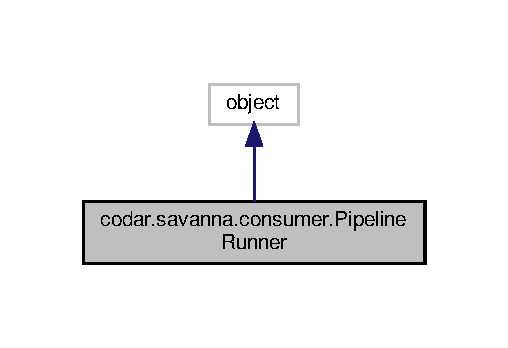
\includegraphics[width=244pt]{classcodar_1_1savanna_1_1consumer_1_1_pipeline_runner__inherit__graph}
\end{center}
\end{figure}


Collaboration diagram for codar.\+savanna.\+consumer.\+Pipeline\+Runner\+:
\nopagebreak
\begin{figure}[H]
\begin{center}
\leavevmode
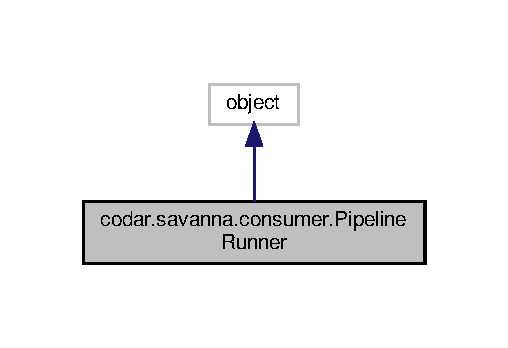
\includegraphics[width=244pt]{classcodar_1_1savanna_1_1consumer_1_1_pipeline_runner__coll__graph}
\end{center}
\end{figure}
\subsection*{Public Member Functions}
\begin{DoxyCompactItemize}
\item 
def \hyperlink{classcodar_1_1savanna_1_1consumer_1_1_pipeline_runner_acf72709f2d294ec9c1136d7ef72d06e4}{\+\_\+\+\_\+init\+\_\+\+\_\+} (self, \hyperlink{classcodar_1_1savanna_1_1consumer_1_1_pipeline_runner_ac2602829f52e9355326fe46748d38e4b}{runner}, \hyperlink{classcodar_1_1savanna_1_1consumer_1_1_pipeline_runner_af0633cf5cd30b71a59f7a5fce860df56}{max\+\_\+nodes}, \hyperlink{classcodar_1_1savanna_1_1consumer_1_1_pipeline_runner_a7f2a92cc8626dbbef1e585178162ddaa}{machine\+\_\+name}, processes\+\_\+per\+\_\+node, status\+\_\+file=None)
\item 
def \hyperlink{classcodar_1_1savanna_1_1consumer_1_1_pipeline_runner_a861447c8086329814e32c709a713f624}{add\+\_\+pipeline} (self, p)
\item 
def \hyperlink{classcodar_1_1savanna_1_1consumer_1_1_pipeline_runner_a62bc31b0b57c9062d05fac14fb50b9b4}{stop} (self)
\item 
def \hyperlink{classcodar_1_1savanna_1_1consumer_1_1_pipeline_runner_a5d7432a5e1b57fa669dbc7391de3c881}{kill\+\_\+all} (self)
\item 
def \hyperlink{classcodar_1_1savanna_1_1consumer_1_1_pipeline_runner_a059b4a5e2c63e6e893a2f1c7862967b3}{run\+\_\+finished} (self, run)
\item 
def \hyperlink{classcodar_1_1savanna_1_1consumer_1_1_pipeline_runner_a4fd8b1e73906734e53fe137f6d808be3}{pipeline\+\_\+finished} (self, pipeline)
\item 
def \hyperlink{classcodar_1_1savanna_1_1consumer_1_1_pipeline_runner_ad8891e29ad84031b9b162b2a7cef918e}{pipeline\+\_\+fatal} (self, pipeline)
\item 
def \hyperlink{classcodar_1_1savanna_1_1consumer_1_1_pipeline_runner_af1fe6b71b44a5e849052a36643444db3}{run\+\_\+pipelines} (self)
\end{DoxyCompactItemize}
\subsection*{Public Attributes}
\begin{DoxyCompactItemize}
\item 
\hyperlink{classcodar_1_1savanna_1_1consumer_1_1_pipeline_runner_af0633cf5cd30b71a59f7a5fce860df56}{max\+\_\+nodes}
\item 
\hyperlink{classcodar_1_1savanna_1_1consumer_1_1_pipeline_runner_a7f2a92cc8626dbbef1e585178162ddaa}{machine\+\_\+name}
\item 
\hyperlink{classcodar_1_1savanna_1_1consumer_1_1_pipeline_runner_a936ec7d8848c12c9c76c1390c19e4923}{ppn}
\item 
\hyperlink{classcodar_1_1savanna_1_1consumer_1_1_pipeline_runner_ac2602829f52e9355326fe46748d38e4b}{runner}
\item 
\hyperlink{classcodar_1_1savanna_1_1consumer_1_1_pipeline_runner_a3434d0d6bd47edebc969215d5bedca53}{job\+\_\+list\+\_\+cv}
\item 
\hyperlink{classcodar_1_1savanna_1_1consumer_1_1_pipeline_runner_a0f41642e362ef2d71e72bdc004185dbe}{job\+\_\+list}
\item 
\hyperlink{classcodar_1_1savanna_1_1consumer_1_1_pipeline_runner_ab95289d735adcde4da6ef3a361f03780}{free\+\_\+cv}
\item 
\hyperlink{classcodar_1_1savanna_1_1consumer_1_1_pipeline_runner_a13e86fda6566c2a958881e3b365ae7a3}{free\+\_\+nodes}
\item 
\hyperlink{classcodar_1_1savanna_1_1consumer_1_1_pipeline_runner_a4eb158f4c9f7326bea855c1d38e5f340}{pipelines\+\_\+lock}
\item 
\hyperlink{classcodar_1_1savanna_1_1consumer_1_1_pipeline_runner_a6a9ac146d408fed1b635cf1d6c3adb5a}{pipelines}
\item 
\hyperlink{classcodar_1_1savanna_1_1consumer_1_1_pipeline_runner_ae8fbcca12ce0cc295d8304c6e9daea5f}{allocated\+\_\+nodes}
\end{DoxyCompactItemize}


\subsection{Detailed Description}
\begin{DoxyVerb}Runner that assumes a homogonous set of nodes. Now only support only
node based limiting (although process limiting can be emulated by setting
process_per_node=1 and max_nodes=max_procs).

Threading model: assumes there could be multiple producer threads calling
add_pipeline, e.g. if using a dynamic job submission model based on
results of previous jobs. Pipelines and each Run in a pipeline are all
executed in separate threads, so their notification callbacks execute in
separate threads, and their threads must be joined before exiting. The
stop and kill_all methods could be called from any of the producer,
Pipeline or Run threads.\end{DoxyVerb}
 

Definition at line 18 of file consumer.\+py.



\subsection{Constructor \& Destructor Documentation}
\mbox{\Hypertarget{classcodar_1_1savanna_1_1consumer_1_1_pipeline_runner_acf72709f2d294ec9c1136d7ef72d06e4}\label{classcodar_1_1savanna_1_1consumer_1_1_pipeline_runner_acf72709f2d294ec9c1136d7ef72d06e4}} 
\index{codar\+::savanna\+::consumer\+::\+Pipeline\+Runner@{codar\+::savanna\+::consumer\+::\+Pipeline\+Runner}!\+\_\+\+\_\+init\+\_\+\+\_\+@{\+\_\+\+\_\+init\+\_\+\+\_\+}}
\index{\+\_\+\+\_\+init\+\_\+\+\_\+@{\+\_\+\+\_\+init\+\_\+\+\_\+}!codar\+::savanna\+::consumer\+::\+Pipeline\+Runner@{codar\+::savanna\+::consumer\+::\+Pipeline\+Runner}}
\subsubsection{\texorpdfstring{\+\_\+\+\_\+init\+\_\+\+\_\+()}{\_\_init\_\_()}}
{\footnotesize\ttfamily def codar.\+savanna.\+consumer.\+Pipeline\+Runner.\+\_\+\+\_\+init\+\_\+\+\_\+ (\begin{DoxyParamCaption}\item[{}]{self,  }\item[{}]{runner,  }\item[{}]{max\+\_\+nodes,  }\item[{}]{machine\+\_\+name,  }\item[{}]{processes\+\_\+per\+\_\+node,  }\item[{}]{status\+\_\+file = {\ttfamily None} }\end{DoxyParamCaption})}



Definition at line 32 of file consumer.\+py.



\subsection{Member Function Documentation}
\mbox{\Hypertarget{classcodar_1_1savanna_1_1consumer_1_1_pipeline_runner_a861447c8086329814e32c709a713f624}\label{classcodar_1_1savanna_1_1consumer_1_1_pipeline_runner_a861447c8086329814e32c709a713f624}} 
\index{codar\+::savanna\+::consumer\+::\+Pipeline\+Runner@{codar\+::savanna\+::consumer\+::\+Pipeline\+Runner}!add\+\_\+pipeline@{add\+\_\+pipeline}}
\index{add\+\_\+pipeline@{add\+\_\+pipeline}!codar\+::savanna\+::consumer\+::\+Pipeline\+Runner@{codar\+::savanna\+::consumer\+::\+Pipeline\+Runner}}
\subsubsection{\texorpdfstring{add\+\_\+pipeline()}{add\_pipeline()}}
{\footnotesize\ttfamily def codar.\+savanna.\+consumer.\+Pipeline\+Runner.\+add\+\_\+pipeline (\begin{DoxyParamCaption}\item[{}]{self,  }\item[{}]{p }\end{DoxyParamCaption})}



Definition at line 73 of file consumer.\+py.

\mbox{\Hypertarget{classcodar_1_1savanna_1_1consumer_1_1_pipeline_runner_a5d7432a5e1b57fa669dbc7391de3c881}\label{classcodar_1_1savanna_1_1consumer_1_1_pipeline_runner_a5d7432a5e1b57fa669dbc7391de3c881}} 
\index{codar\+::savanna\+::consumer\+::\+Pipeline\+Runner@{codar\+::savanna\+::consumer\+::\+Pipeline\+Runner}!kill\+\_\+all@{kill\+\_\+all}}
\index{kill\+\_\+all@{kill\+\_\+all}!codar\+::savanna\+::consumer\+::\+Pipeline\+Runner@{codar\+::savanna\+::consumer\+::\+Pipeline\+Runner}}
\subsubsection{\texorpdfstring{kill\+\_\+all()}{kill\_all()}}
{\footnotesize\ttfamily def codar.\+savanna.\+consumer.\+Pipeline\+Runner.\+kill\+\_\+all (\begin{DoxyParamCaption}\item[{}]{self }\end{DoxyParamCaption})}

\begin{DoxyVerb}Kill all running processes spawned by this consumer and don't
start any new processes.\end{DoxyVerb}
 

Definition at line 114 of file consumer.\+py.

\mbox{\Hypertarget{classcodar_1_1savanna_1_1consumer_1_1_pipeline_runner_ad8891e29ad84031b9b162b2a7cef918e}\label{classcodar_1_1savanna_1_1consumer_1_1_pipeline_runner_ad8891e29ad84031b9b162b2a7cef918e}} 
\index{codar\+::savanna\+::consumer\+::\+Pipeline\+Runner@{codar\+::savanna\+::consumer\+::\+Pipeline\+Runner}!pipeline\+\_\+fatal@{pipeline\+\_\+fatal}}
\index{pipeline\+\_\+fatal@{pipeline\+\_\+fatal}!codar\+::savanna\+::consumer\+::\+Pipeline\+Runner@{codar\+::savanna\+::consumer\+::\+Pipeline\+Runner}}
\subsubsection{\texorpdfstring{pipeline\+\_\+fatal()}{pipeline\_fatal()}}
{\footnotesize\ttfamily def codar.\+savanna.\+consumer.\+Pipeline\+Runner.\+pipeline\+\_\+fatal (\begin{DoxyParamCaption}\item[{}]{self,  }\item[{}]{pipeline }\end{DoxyParamCaption})}



Definition at line 190 of file consumer.\+py.

\mbox{\Hypertarget{classcodar_1_1savanna_1_1consumer_1_1_pipeline_runner_a4fd8b1e73906734e53fe137f6d808be3}\label{classcodar_1_1savanna_1_1consumer_1_1_pipeline_runner_a4fd8b1e73906734e53fe137f6d808be3}} 
\index{codar\+::savanna\+::consumer\+::\+Pipeline\+Runner@{codar\+::savanna\+::consumer\+::\+Pipeline\+Runner}!pipeline\+\_\+finished@{pipeline\+\_\+finished}}
\index{pipeline\+\_\+finished@{pipeline\+\_\+finished}!codar\+::savanna\+::consumer\+::\+Pipeline\+Runner@{codar\+::savanna\+::consumer\+::\+Pipeline\+Runner}}
\subsubsection{\texorpdfstring{pipeline\+\_\+finished()}{pipeline\_finished()}}
{\footnotesize\ttfamily def codar.\+savanna.\+consumer.\+Pipeline\+Runner.\+pipeline\+\_\+finished (\begin{DoxyParamCaption}\item[{}]{self,  }\item[{}]{pipeline }\end{DoxyParamCaption})}

\begin{DoxyVerb}Monitor thread(s) should call this as pipelines complete.\end{DoxyVerb}
 

Definition at line 164 of file consumer.\+py.

\mbox{\Hypertarget{classcodar_1_1savanna_1_1consumer_1_1_pipeline_runner_a059b4a5e2c63e6e893a2f1c7862967b3}\label{classcodar_1_1savanna_1_1consumer_1_1_pipeline_runner_a059b4a5e2c63e6e893a2f1c7862967b3}} 
\index{codar\+::savanna\+::consumer\+::\+Pipeline\+Runner@{codar\+::savanna\+::consumer\+::\+Pipeline\+Runner}!run\+\_\+finished@{run\+\_\+finished}}
\index{run\+\_\+finished@{run\+\_\+finished}!codar\+::savanna\+::consumer\+::\+Pipeline\+Runner@{codar\+::savanna\+::consumer\+::\+Pipeline\+Runner}}
\subsubsection{\texorpdfstring{run\+\_\+finished()}{run\_finished()}}
{\footnotesize\ttfamily def codar.\+savanna.\+consumer.\+Pipeline\+Runner.\+run\+\_\+finished (\begin{DoxyParamCaption}\item[{}]{self,  }\item[{}]{run }\end{DoxyParamCaption})}

\begin{DoxyVerb}TO BE DEPRECATED.
Monitor thread(s) should call this as runs
complete. To be deprecated, as the functionality fails when
node_layout is set to node-sharing.

This means that for node_exclusive, resources held by a run are not
released when the run terminates. For kill_on_partial_failure=False,
this could lead to unused resources, which is ok.\end{DoxyVerb}
 

Definition at line 148 of file consumer.\+py.

\mbox{\Hypertarget{classcodar_1_1savanna_1_1consumer_1_1_pipeline_runner_af1fe6b71b44a5e849052a36643444db3}\label{classcodar_1_1savanna_1_1consumer_1_1_pipeline_runner_af1fe6b71b44a5e849052a36643444db3}} 
\index{codar\+::savanna\+::consumer\+::\+Pipeline\+Runner@{codar\+::savanna\+::consumer\+::\+Pipeline\+Runner}!run\+\_\+pipelines@{run\+\_\+pipelines}}
\index{run\+\_\+pipelines@{run\+\_\+pipelines}!codar\+::savanna\+::consumer\+::\+Pipeline\+Runner@{codar\+::savanna\+::consumer\+::\+Pipeline\+Runner}}
\subsubsection{\texorpdfstring{run\+\_\+pipelines()}{run\_pipelines()}}
{\footnotesize\ttfamily def codar.\+savanna.\+consumer.\+Pipeline\+Runner.\+run\+\_\+pipelines (\begin{DoxyParamCaption}\item[{}]{self }\end{DoxyParamCaption})}

\begin{DoxyVerb}Main loop of consumer thread. Does not return until all child
threads are complete.\end{DoxyVerb}
 

Definition at line 194 of file consumer.\+py.

\mbox{\Hypertarget{classcodar_1_1savanna_1_1consumer_1_1_pipeline_runner_a62bc31b0b57c9062d05fac14fb50b9b4}\label{classcodar_1_1savanna_1_1consumer_1_1_pipeline_runner_a62bc31b0b57c9062d05fac14fb50b9b4}} 
\index{codar\+::savanna\+::consumer\+::\+Pipeline\+Runner@{codar\+::savanna\+::consumer\+::\+Pipeline\+Runner}!stop@{stop}}
\index{stop@{stop}!codar\+::savanna\+::consumer\+::\+Pipeline\+Runner@{codar\+::savanna\+::consumer\+::\+Pipeline\+Runner}}
\subsubsection{\texorpdfstring{stop()}{stop()}}
{\footnotesize\ttfamily def codar.\+savanna.\+consumer.\+Pipeline\+Runner.\+stop (\begin{DoxyParamCaption}\item[{}]{self }\end{DoxyParamCaption})}

\begin{DoxyVerb}Signal to stop when all pipelines are finished. Don't allow adding
new pipelines.\end{DoxyVerb}
 

Definition at line 105 of file consumer.\+py.



\subsection{Member Data Documentation}
\mbox{\Hypertarget{classcodar_1_1savanna_1_1consumer_1_1_pipeline_runner_ae8fbcca12ce0cc295d8304c6e9daea5f}\label{classcodar_1_1savanna_1_1consumer_1_1_pipeline_runner_ae8fbcca12ce0cc295d8304c6e9daea5f}} 
\index{codar\+::savanna\+::consumer\+::\+Pipeline\+Runner@{codar\+::savanna\+::consumer\+::\+Pipeline\+Runner}!allocated\+\_\+nodes@{allocated\+\_\+nodes}}
\index{allocated\+\_\+nodes@{allocated\+\_\+nodes}!codar\+::savanna\+::consumer\+::\+Pipeline\+Runner@{codar\+::savanna\+::consumer\+::\+Pipeline\+Runner}}
\subsubsection{\texorpdfstring{allocated\+\_\+nodes}{allocated\_nodes}}
{\footnotesize\ttfamily codar.\+savanna.\+consumer.\+Pipeline\+Runner.\+allocated\+\_\+nodes}



Definition at line 60 of file consumer.\+py.

\mbox{\Hypertarget{classcodar_1_1savanna_1_1consumer_1_1_pipeline_runner_ab95289d735adcde4da6ef3a361f03780}\label{classcodar_1_1savanna_1_1consumer_1_1_pipeline_runner_ab95289d735adcde4da6ef3a361f03780}} 
\index{codar\+::savanna\+::consumer\+::\+Pipeline\+Runner@{codar\+::savanna\+::consumer\+::\+Pipeline\+Runner}!free\+\_\+cv@{free\+\_\+cv}}
\index{free\+\_\+cv@{free\+\_\+cv}!codar\+::savanna\+::consumer\+::\+Pipeline\+Runner@{codar\+::savanna\+::consumer\+::\+Pipeline\+Runner}}
\subsubsection{\texorpdfstring{free\+\_\+cv}{free\_cv}}
{\footnotesize\ttfamily codar.\+savanna.\+consumer.\+Pipeline\+Runner.\+free\+\_\+cv}



Definition at line 47 of file consumer.\+py.

\mbox{\Hypertarget{classcodar_1_1savanna_1_1consumer_1_1_pipeline_runner_a13e86fda6566c2a958881e3b365ae7a3}\label{classcodar_1_1savanna_1_1consumer_1_1_pipeline_runner_a13e86fda6566c2a958881e3b365ae7a3}} 
\index{codar\+::savanna\+::consumer\+::\+Pipeline\+Runner@{codar\+::savanna\+::consumer\+::\+Pipeline\+Runner}!free\+\_\+nodes@{free\+\_\+nodes}}
\index{free\+\_\+nodes@{free\+\_\+nodes}!codar\+::savanna\+::consumer\+::\+Pipeline\+Runner@{codar\+::savanna\+::consumer\+::\+Pipeline\+Runner}}
\subsubsection{\texorpdfstring{free\+\_\+nodes}{free\_nodes}}
{\footnotesize\ttfamily codar.\+savanna.\+consumer.\+Pipeline\+Runner.\+free\+\_\+nodes}



Definition at line 48 of file consumer.\+py.

\mbox{\Hypertarget{classcodar_1_1savanna_1_1consumer_1_1_pipeline_runner_a0f41642e362ef2d71e72bdc004185dbe}\label{classcodar_1_1savanna_1_1consumer_1_1_pipeline_runner_a0f41642e362ef2d71e72bdc004185dbe}} 
\index{codar\+::savanna\+::consumer\+::\+Pipeline\+Runner@{codar\+::savanna\+::consumer\+::\+Pipeline\+Runner}!job\+\_\+list@{job\+\_\+list}}
\index{job\+\_\+list@{job\+\_\+list}!codar\+::savanna\+::consumer\+::\+Pipeline\+Runner@{codar\+::savanna\+::consumer\+::\+Pipeline\+Runner}}
\subsubsection{\texorpdfstring{job\+\_\+list}{job\_list}}
{\footnotesize\ttfamily codar.\+savanna.\+consumer.\+Pipeline\+Runner.\+job\+\_\+list}



Definition at line 45 of file consumer.\+py.

\mbox{\Hypertarget{classcodar_1_1savanna_1_1consumer_1_1_pipeline_runner_a3434d0d6bd47edebc969215d5bedca53}\label{classcodar_1_1savanna_1_1consumer_1_1_pipeline_runner_a3434d0d6bd47edebc969215d5bedca53}} 
\index{codar\+::savanna\+::consumer\+::\+Pipeline\+Runner@{codar\+::savanna\+::consumer\+::\+Pipeline\+Runner}!job\+\_\+list\+\_\+cv@{job\+\_\+list\+\_\+cv}}
\index{job\+\_\+list\+\_\+cv@{job\+\_\+list\+\_\+cv}!codar\+::savanna\+::consumer\+::\+Pipeline\+Runner@{codar\+::savanna\+::consumer\+::\+Pipeline\+Runner}}
\subsubsection{\texorpdfstring{job\+\_\+list\+\_\+cv}{job\_list\_cv}}
{\footnotesize\ttfamily codar.\+savanna.\+consumer.\+Pipeline\+Runner.\+job\+\_\+list\+\_\+cv}



Definition at line 43 of file consumer.\+py.

\mbox{\Hypertarget{classcodar_1_1savanna_1_1consumer_1_1_pipeline_runner_a7f2a92cc8626dbbef1e585178162ddaa}\label{classcodar_1_1savanna_1_1consumer_1_1_pipeline_runner_a7f2a92cc8626dbbef1e585178162ddaa}} 
\index{codar\+::savanna\+::consumer\+::\+Pipeline\+Runner@{codar\+::savanna\+::consumer\+::\+Pipeline\+Runner}!machine\+\_\+name@{machine\+\_\+name}}
\index{machine\+\_\+name@{machine\+\_\+name}!codar\+::savanna\+::consumer\+::\+Pipeline\+Runner@{codar\+::savanna\+::consumer\+::\+Pipeline\+Runner}}
\subsubsection{\texorpdfstring{machine\+\_\+name}{machine\_name}}
{\footnotesize\ttfamily codar.\+savanna.\+consumer.\+Pipeline\+Runner.\+machine\+\_\+name}



Definition at line 34 of file consumer.\+py.

\mbox{\Hypertarget{classcodar_1_1savanna_1_1consumer_1_1_pipeline_runner_af0633cf5cd30b71a59f7a5fce860df56}\label{classcodar_1_1savanna_1_1consumer_1_1_pipeline_runner_af0633cf5cd30b71a59f7a5fce860df56}} 
\index{codar\+::savanna\+::consumer\+::\+Pipeline\+Runner@{codar\+::savanna\+::consumer\+::\+Pipeline\+Runner}!max\+\_\+nodes@{max\+\_\+nodes}}
\index{max\+\_\+nodes@{max\+\_\+nodes}!codar\+::savanna\+::consumer\+::\+Pipeline\+Runner@{codar\+::savanna\+::consumer\+::\+Pipeline\+Runner}}
\subsubsection{\texorpdfstring{max\+\_\+nodes}{max\_nodes}}
{\footnotesize\ttfamily codar.\+savanna.\+consumer.\+Pipeline\+Runner.\+max\+\_\+nodes}



Definition at line 33 of file consumer.\+py.

\mbox{\Hypertarget{classcodar_1_1savanna_1_1consumer_1_1_pipeline_runner_a6a9ac146d408fed1b635cf1d6c3adb5a}\label{classcodar_1_1savanna_1_1consumer_1_1_pipeline_runner_a6a9ac146d408fed1b635cf1d6c3adb5a}} 
\index{codar\+::savanna\+::consumer\+::\+Pipeline\+Runner@{codar\+::savanna\+::consumer\+::\+Pipeline\+Runner}!pipelines@{pipelines}}
\index{pipelines@{pipelines}!codar\+::savanna\+::consumer\+::\+Pipeline\+Runner@{codar\+::savanna\+::consumer\+::\+Pipeline\+Runner}}
\subsubsection{\texorpdfstring{pipelines}{pipelines}}
{\footnotesize\ttfamily codar.\+savanna.\+consumer.\+Pipeline\+Runner.\+pipelines}



Definition at line 51 of file consumer.\+py.

\mbox{\Hypertarget{classcodar_1_1savanna_1_1consumer_1_1_pipeline_runner_a4eb158f4c9f7326bea855c1d38e5f340}\label{classcodar_1_1savanna_1_1consumer_1_1_pipeline_runner_a4eb158f4c9f7326bea855c1d38e5f340}} 
\index{codar\+::savanna\+::consumer\+::\+Pipeline\+Runner@{codar\+::savanna\+::consumer\+::\+Pipeline\+Runner}!pipelines\+\_\+lock@{pipelines\+\_\+lock}}
\index{pipelines\+\_\+lock@{pipelines\+\_\+lock}!codar\+::savanna\+::consumer\+::\+Pipeline\+Runner@{codar\+::savanna\+::consumer\+::\+Pipeline\+Runner}}
\subsubsection{\texorpdfstring{pipelines\+\_\+lock}{pipelines\_lock}}
{\footnotesize\ttfamily codar.\+savanna.\+consumer.\+Pipeline\+Runner.\+pipelines\+\_\+lock}



Definition at line 50 of file consumer.\+py.

\mbox{\Hypertarget{classcodar_1_1savanna_1_1consumer_1_1_pipeline_runner_a936ec7d8848c12c9c76c1390c19e4923}\label{classcodar_1_1savanna_1_1consumer_1_1_pipeline_runner_a936ec7d8848c12c9c76c1390c19e4923}} 
\index{codar\+::savanna\+::consumer\+::\+Pipeline\+Runner@{codar\+::savanna\+::consumer\+::\+Pipeline\+Runner}!ppn@{ppn}}
\index{ppn@{ppn}!codar\+::savanna\+::consumer\+::\+Pipeline\+Runner@{codar\+::savanna\+::consumer\+::\+Pipeline\+Runner}}
\subsubsection{\texorpdfstring{ppn}{ppn}}
{\footnotesize\ttfamily codar.\+savanna.\+consumer.\+Pipeline\+Runner.\+ppn}



Definition at line 35 of file consumer.\+py.

\mbox{\Hypertarget{classcodar_1_1savanna_1_1consumer_1_1_pipeline_runner_ac2602829f52e9355326fe46748d38e4b}\label{classcodar_1_1savanna_1_1consumer_1_1_pipeline_runner_ac2602829f52e9355326fe46748d38e4b}} 
\index{codar\+::savanna\+::consumer\+::\+Pipeline\+Runner@{codar\+::savanna\+::consumer\+::\+Pipeline\+Runner}!runner@{runner}}
\index{runner@{runner}!codar\+::savanna\+::consumer\+::\+Pipeline\+Runner@{codar\+::savanna\+::consumer\+::\+Pipeline\+Runner}}
\subsubsection{\texorpdfstring{runner}{runner}}
{\footnotesize\ttfamily codar.\+savanna.\+consumer.\+Pipeline\+Runner.\+runner}



Definition at line 36 of file consumer.\+py.



The documentation for this class was generated from the following file\+:\begin{DoxyCompactItemize}
\item 
\hyperlink{consumer_8py}{consumer.\+py}\end{DoxyCompactItemize}

\hypertarget{classcodar_1_1savanna_1_1status_1_1_pipeline_state}{}\section{codar.\+savanna.\+status.\+Pipeline\+State Class Reference}
\label{classcodar_1_1savanna_1_1status_1_1_pipeline_state}\index{codar.\+savanna.\+status.\+Pipeline\+State@{codar.\+savanna.\+status.\+Pipeline\+State}}


Inheritance diagram for codar.\+savanna.\+status.\+Pipeline\+State\+:
\nopagebreak
\begin{figure}[H]
\begin{center}
\leavevmode
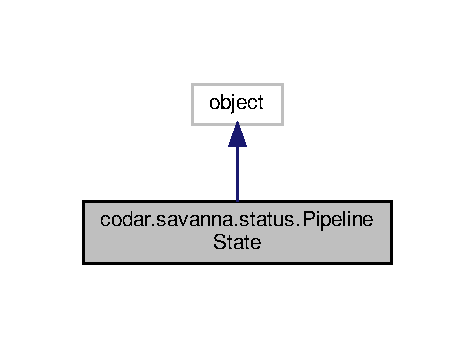
\includegraphics[width=228pt]{classcodar_1_1savanna_1_1status_1_1_pipeline_state__inherit__graph}
\end{center}
\end{figure}


Collaboration diagram for codar.\+savanna.\+status.\+Pipeline\+State\+:
\nopagebreak
\begin{figure}[H]
\begin{center}
\leavevmode
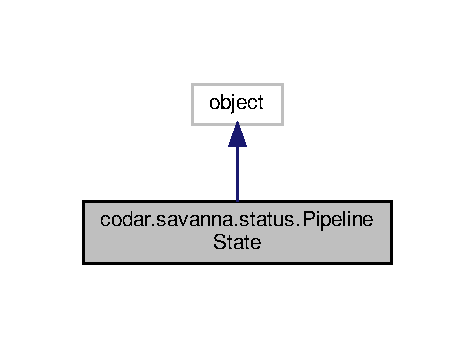
\includegraphics[width=228pt]{classcodar_1_1savanna_1_1status_1_1_pipeline_state__coll__graph}
\end{center}
\end{figure}
\subsection*{Public Member Functions}
\begin{DoxyCompactItemize}
\item 
def \hyperlink{classcodar_1_1savanna_1_1status_1_1_pipeline_state_aad524111d3971ff923bbe0fb1846d2e0}{\+\_\+\+\_\+init\+\_\+\+\_\+} (self, pipeline\+\_\+id, \hyperlink{classcodar_1_1savanna_1_1status_1_1_pipeline_state_a88ffca97c0ff1a0f41874cbeb60b90d3}{state}, \hyperlink{classcodar_1_1savanna_1_1status_1_1_pipeline_state_ac5a9c042a32b7e3201392bdc680ef42e}{reason}=None, \hyperlink{classcodar_1_1savanna_1_1status_1_1_pipeline_state_a5c8ed429b9840e57e11bf69eaa18c9c8}{return\+\_\+codes}=None)
\item 
def \hyperlink{classcodar_1_1savanna_1_1status_1_1_pipeline_state_a6bc3b110734ec87c57ea209e8e34a1de}{as\+\_\+data} (self)
\end{DoxyCompactItemize}
\subsection*{Public Attributes}
\begin{DoxyCompactItemize}
\item 
\hyperlink{classcodar_1_1savanna_1_1status_1_1_pipeline_state_a84555aff70ced0a148ecb0b19d9421e3}{id}
\item 
\hyperlink{classcodar_1_1savanna_1_1status_1_1_pipeline_state_a88ffca97c0ff1a0f41874cbeb60b90d3}{state}
\item 
\hyperlink{classcodar_1_1savanna_1_1status_1_1_pipeline_state_ac5a9c042a32b7e3201392bdc680ef42e}{reason}
\item 
\hyperlink{classcodar_1_1savanna_1_1status_1_1_pipeline_state_a5c8ed429b9840e57e11bf69eaa18c9c8}{return\+\_\+codes}
\end{DoxyCompactItemize}


\subsection{Detailed Description}


Definition at line 48 of file status.\+py.



\subsection{Constructor \& Destructor Documentation}
\mbox{\Hypertarget{classcodar_1_1savanna_1_1status_1_1_pipeline_state_aad524111d3971ff923bbe0fb1846d2e0}\label{classcodar_1_1savanna_1_1status_1_1_pipeline_state_aad524111d3971ff923bbe0fb1846d2e0}} 
\index{codar\+::savanna\+::status\+::\+Pipeline\+State@{codar\+::savanna\+::status\+::\+Pipeline\+State}!\+\_\+\+\_\+init\+\_\+\+\_\+@{\+\_\+\+\_\+init\+\_\+\+\_\+}}
\index{\+\_\+\+\_\+init\+\_\+\+\_\+@{\+\_\+\+\_\+init\+\_\+\+\_\+}!codar\+::savanna\+::status\+::\+Pipeline\+State@{codar\+::savanna\+::status\+::\+Pipeline\+State}}
\subsubsection{\texorpdfstring{\+\_\+\+\_\+init\+\_\+\+\_\+()}{\_\_init\_\_()}}
{\footnotesize\ttfamily def codar.\+savanna.\+status.\+Pipeline\+State.\+\_\+\+\_\+init\+\_\+\+\_\+ (\begin{DoxyParamCaption}\item[{}]{self,  }\item[{}]{pipeline\+\_\+id,  }\item[{}]{state,  }\item[{}]{reason = {\ttfamily None},  }\item[{}]{return\+\_\+codes = {\ttfamily None} }\end{DoxyParamCaption})}



Definition at line 49 of file status.\+py.



\subsection{Member Function Documentation}
\mbox{\Hypertarget{classcodar_1_1savanna_1_1status_1_1_pipeline_state_a6bc3b110734ec87c57ea209e8e34a1de}\label{classcodar_1_1savanna_1_1status_1_1_pipeline_state_a6bc3b110734ec87c57ea209e8e34a1de}} 
\index{codar\+::savanna\+::status\+::\+Pipeline\+State@{codar\+::savanna\+::status\+::\+Pipeline\+State}!as\+\_\+data@{as\+\_\+data}}
\index{as\+\_\+data@{as\+\_\+data}!codar\+::savanna\+::status\+::\+Pipeline\+State@{codar\+::savanna\+::status\+::\+Pipeline\+State}}
\subsubsection{\texorpdfstring{as\+\_\+data()}{as\_data()}}
{\footnotesize\ttfamily def codar.\+savanna.\+status.\+Pipeline\+State.\+as\+\_\+data (\begin{DoxyParamCaption}\item[{}]{self }\end{DoxyParamCaption})}



Definition at line 55 of file status.\+py.



\subsection{Member Data Documentation}
\mbox{\Hypertarget{classcodar_1_1savanna_1_1status_1_1_pipeline_state_a84555aff70ced0a148ecb0b19d9421e3}\label{classcodar_1_1savanna_1_1status_1_1_pipeline_state_a84555aff70ced0a148ecb0b19d9421e3}} 
\index{codar\+::savanna\+::status\+::\+Pipeline\+State@{codar\+::savanna\+::status\+::\+Pipeline\+State}!id@{id}}
\index{id@{id}!codar\+::savanna\+::status\+::\+Pipeline\+State@{codar\+::savanna\+::status\+::\+Pipeline\+State}}
\subsubsection{\texorpdfstring{id}{id}}
{\footnotesize\ttfamily codar.\+savanna.\+status.\+Pipeline\+State.\+id}



Definition at line 50 of file status.\+py.

\mbox{\Hypertarget{classcodar_1_1savanna_1_1status_1_1_pipeline_state_ac5a9c042a32b7e3201392bdc680ef42e}\label{classcodar_1_1savanna_1_1status_1_1_pipeline_state_ac5a9c042a32b7e3201392bdc680ef42e}} 
\index{codar\+::savanna\+::status\+::\+Pipeline\+State@{codar\+::savanna\+::status\+::\+Pipeline\+State}!reason@{reason}}
\index{reason@{reason}!codar\+::savanna\+::status\+::\+Pipeline\+State@{codar\+::savanna\+::status\+::\+Pipeline\+State}}
\subsubsection{\texorpdfstring{reason}{reason}}
{\footnotesize\ttfamily codar.\+savanna.\+status.\+Pipeline\+State.\+reason}



Definition at line 52 of file status.\+py.

\mbox{\Hypertarget{classcodar_1_1savanna_1_1status_1_1_pipeline_state_a5c8ed429b9840e57e11bf69eaa18c9c8}\label{classcodar_1_1savanna_1_1status_1_1_pipeline_state_a5c8ed429b9840e57e11bf69eaa18c9c8}} 
\index{codar\+::savanna\+::status\+::\+Pipeline\+State@{codar\+::savanna\+::status\+::\+Pipeline\+State}!return\+\_\+codes@{return\+\_\+codes}}
\index{return\+\_\+codes@{return\+\_\+codes}!codar\+::savanna\+::status\+::\+Pipeline\+State@{codar\+::savanna\+::status\+::\+Pipeline\+State}}
\subsubsection{\texorpdfstring{return\+\_\+codes}{return\_codes}}
{\footnotesize\ttfamily codar.\+savanna.\+status.\+Pipeline\+State.\+return\+\_\+codes}



Definition at line 53 of file status.\+py.

\mbox{\Hypertarget{classcodar_1_1savanna_1_1status_1_1_pipeline_state_a88ffca97c0ff1a0f41874cbeb60b90d3}\label{classcodar_1_1savanna_1_1status_1_1_pipeline_state_a88ffca97c0ff1a0f41874cbeb60b90d3}} 
\index{codar\+::savanna\+::status\+::\+Pipeline\+State@{codar\+::savanna\+::status\+::\+Pipeline\+State}!state@{state}}
\index{state@{state}!codar\+::savanna\+::status\+::\+Pipeline\+State@{codar\+::savanna\+::status\+::\+Pipeline\+State}}
\subsubsection{\texorpdfstring{state}{state}}
{\footnotesize\ttfamily codar.\+savanna.\+status.\+Pipeline\+State.\+state}



Definition at line 51 of file status.\+py.



The documentation for this class was generated from the following file\+:\begin{DoxyCompactItemize}
\item 
savanna/\hyperlink{savanna_2status_8py}{status.\+py}\end{DoxyCompactItemize}

\hypertarget{classcodar_1_1savanna_1_1model_1_1_run}{}\section{codar.\+savanna.\+model.\+Run Class Reference}
\label{classcodar_1_1savanna_1_1model_1_1_run}\index{codar.\+savanna.\+model.\+Run@{codar.\+savanna.\+model.\+Run}}


Inheritance diagram for codar.\+savanna.\+model.\+Run\+:
\nopagebreak
\begin{figure}[H]
\begin{center}
\leavevmode
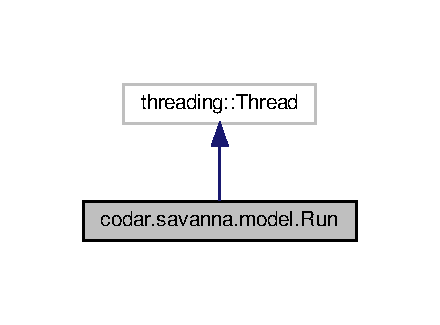
\includegraphics[width=211pt]{classcodar_1_1savanna_1_1model_1_1_run__inherit__graph}
\end{center}
\end{figure}


Collaboration diagram for codar.\+savanna.\+model.\+Run\+:
\nopagebreak
\begin{figure}[H]
\begin{center}
\leavevmode
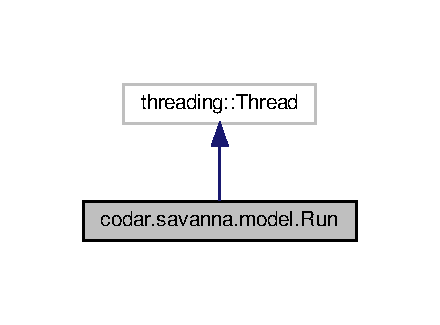
\includegraphics[width=211pt]{classcodar_1_1savanna_1_1model_1_1_run__coll__graph}
\end{center}
\end{figure}
\subsection*{Public Member Functions}
\begin{DoxyCompactItemize}
\item 
def \hyperlink{classcodar_1_1savanna_1_1model_1_1_run_a796853700dcd65de0394fa521b0d5c21}{\+\_\+\+\_\+init\+\_\+\+\_\+} (self, \hyperlink{classcodar_1_1savanna_1_1model_1_1_run_a135987f2d76c2b733237f9128df90b55}{name}, \hyperlink{classcodar_1_1savanna_1_1model_1_1_run_af3869303fd11d0eea96c69adda61ffbf}{exe}, \hyperlink{classcodar_1_1savanna_1_1model_1_1_run_a2e95781a43d4b3146b10b98c6df429a4}{args}, \hyperlink{classcodar_1_1savanna_1_1model_1_1_run_a530b04dbe3d3a1feea2e970c2c7cc4a0}{sched\+\_\+args}, \hyperlink{classcodar_1_1savanna_1_1model_1_1_run_aca381aeba4c386241910c0ecffa97189}{env}, \hyperlink{classcodar_1_1savanna_1_1model_1_1_run_aa7acd6225eca948ecf25d122d1cca66d}{working\+\_\+dir}, \hyperlink{classcodar_1_1savanna_1_1model_1_1_run_abb445426d12c93f4b0fffaad44e46f78}{timeout}=None, \hyperlink{classcodar_1_1savanna_1_1model_1_1_run_afcec81e8eeb87cecb91a1101ad0b688a}{nprocs}=1, \hyperlink{classcodar_1_1savanna_1_1model_1_1_run_a558ab10e87015683e656fd0b8f9ea433}{res\+\_\+set}=None, \hyperlink{classcodar_1_1savanna_1_1model_1_1_run_a94ef5e9dc24c400534dc80d80ec5aeb0}{stdout\+\_\+path}=None, \hyperlink{classcodar_1_1savanna_1_1model_1_1_run_a55aa41b42450a290a508a17d57fe209d}{stderr\+\_\+path}=None, \hyperlink{classcodar_1_1savanna_1_1model_1_1_run_a497134b579d440c7b79281d57cc93aa7}{return\+\_\+path}=None, \hyperlink{classcodar_1_1savanna_1_1model_1_1_run_af0cf79c5f8c52048604391d984bd48bc}{walltime\+\_\+path}=None, \hyperlink{classcodar_1_1savanna_1_1model_1_1_run_adccd41ed98f61dd602822096a1bdf517}{log\+\_\+prefix}=None, \hyperlink{classcodar_1_1savanna_1_1model_1_1_run_a386d4496d2923fb080c5f43dd325c87b}{sleep\+\_\+after}=None, \hyperlink{classcodar_1_1savanna_1_1model_1_1_run_aa5202a9a7a6a7b928fbf808eab8defb5}{depends\+\_\+on\+\_\+runs}=None, \hyperlink{classcodar_1_1savanna_1_1model_1_1_run_af216be8820a6bedc05b5e613a03c862d}{hostfile}=None, \hyperlink{classcodar_1_1savanna_1_1model_1_1_run_a687ceaaa3bd97a392487ea57b662e7a3}{runner\+\_\+override}=False)
\item 
def \hyperlink{classcodar_1_1savanna_1_1model_1_1_run_a8fab27229098b129079844b82035eab2}{from\+\_\+data} (cls, data)
\item 
def \hyperlink{classcodar_1_1savanna_1_1model_1_1_run_a1624f958c672fd64cbb2e4d124c69890}{mpmd\+\_\+run} (cls, runs)
\item 
def \hyperlink{classcodar_1_1savanna_1_1model_1_1_run_aac3822b6e9166a3c2c5ea7906d89ece9}{set\+\_\+runner} (self, \hyperlink{classcodar_1_1savanna_1_1model_1_1_run_a4e689edb49d16bcae268fbda092bbe9c}{runner})
\item 
def \hyperlink{classcodar_1_1savanna_1_1model_1_1_run_a3d5293dbe910c5e940e71ceeeb82778d}{timed\+\_\+out} (self)
\item 
def \hyperlink{classcodar_1_1savanna_1_1model_1_1_run_abf7413759a4e4d456e978e5bade25e02}{killed} (self)
\item 
def \hyperlink{classcodar_1_1savanna_1_1model_1_1_run_a3e764a9c156037997b107a268716cf7e}{exception} (self)
\item 
def \hyperlink{classcodar_1_1savanna_1_1model_1_1_run_a5b08f9604e4010ab32059e3291448cda}{succeeded} (self)
\item 
def \hyperlink{classcodar_1_1savanna_1_1model_1_1_run_a73899dead2dbe21ee0242edf9e21515d}{add\+\_\+callback} (self, fn)
\item 
def \hyperlink{classcodar_1_1savanna_1_1model_1_1_run_a470a9f2082dcf6244fdf330dc8dc7990}{remove\+\_\+callback} (self, fn)
\item 
def \hyperlink{classcodar_1_1savanna_1_1model_1_1_run_a90816a0d12240402ca7b5754ffc44242}{run} (self)
\item 
def \hyperlink{classcodar_1_1savanna_1_1model_1_1_run_a734d77c85281aa6b2d76ec798575c52b}{kill} (self)
\item 
def \hyperlink{classcodar_1_1savanna_1_1model_1_1_run_ad58affb918ea0222f8e53196b68f6f86}{get\+\_\+returncode} (self)
\item 
def \hyperlink{classcodar_1_1savanna_1_1model_1_1_run_a996441976a9c4facd1c4de9eb32be24a}{get\+\_\+pid} (self)
\item 
def \hyperlink{classcodar_1_1savanna_1_1model_1_1_run_a079f9410453bd7459a8d0acdc891c6cf}{close} (self)
\item 
def \hyperlink{classcodar_1_1savanna_1_1model_1_1_run_a9f413d6685194f969cc686f6e829d8a9}{join} (self)
\item 
def \hyperlink{classcodar_1_1savanna_1_1model_1_1_run_a3b135416fb501328bba834045d2265b0}{get\+\_\+nodes\+\_\+used} (self)
\item 
def \hyperlink{classcodar_1_1savanna_1_1model_1_1_run_a1c7234a57ae8bcb81fdec643f3825b31}{create\+\_\+node\+\_\+config} (self)
\end{DoxyCompactItemize}
\subsection*{Public Attributes}
\begin{DoxyCompactItemize}
\item 
\hyperlink{classcodar_1_1savanna_1_1model_1_1_run_a135987f2d76c2b733237f9128df90b55}{name}
\item 
\hyperlink{classcodar_1_1savanna_1_1model_1_1_run_af3869303fd11d0eea96c69adda61ffbf}{exe}
\item 
\hyperlink{classcodar_1_1savanna_1_1model_1_1_run_a2e95781a43d4b3146b10b98c6df429a4}{args}
\item 
\hyperlink{classcodar_1_1savanna_1_1model_1_1_run_a530b04dbe3d3a1feea2e970c2c7cc4a0}{sched\+\_\+args}
\item 
\hyperlink{classcodar_1_1savanna_1_1model_1_1_run_aca381aeba4c386241910c0ecffa97189}{env}
\item 
\hyperlink{classcodar_1_1savanna_1_1model_1_1_run_aa7acd6225eca948ecf25d122d1cca66d}{working\+\_\+dir}
\item 
\hyperlink{classcodar_1_1savanna_1_1model_1_1_run_abb445426d12c93f4b0fffaad44e46f78}{timeout}
\item 
\hyperlink{classcodar_1_1savanna_1_1model_1_1_run_afcec81e8eeb87cecb91a1101ad0b688a}{nprocs}
\item 
\hyperlink{classcodar_1_1savanna_1_1model_1_1_run_a558ab10e87015683e656fd0b8f9ea433}{res\+\_\+set}
\item 
\hyperlink{classcodar_1_1savanna_1_1model_1_1_run_a94ef5e9dc24c400534dc80d80ec5aeb0}{stdout\+\_\+path}
\item 
\hyperlink{classcodar_1_1savanna_1_1model_1_1_run_a55aa41b42450a290a508a17d57fe209d}{stderr\+\_\+path}
\item 
\hyperlink{classcodar_1_1savanna_1_1model_1_1_run_a497134b579d440c7b79281d57cc93aa7}{return\+\_\+path}
\item 
\hyperlink{classcodar_1_1savanna_1_1model_1_1_run_af0cf79c5f8c52048604391d984bd48bc}{walltime\+\_\+path}
\item 
\hyperlink{classcodar_1_1savanna_1_1model_1_1_run_a386d4496d2923fb080c5f43dd325c87b}{sleep\+\_\+after}
\item 
\hyperlink{classcodar_1_1savanna_1_1model_1_1_run_adccd41ed98f61dd602822096a1bdf517}{log\+\_\+prefix}
\item 
\hyperlink{classcodar_1_1savanna_1_1model_1_1_run_a4e689edb49d16bcae268fbda092bbe9c}{runner}
\item 
\hyperlink{classcodar_1_1savanna_1_1model_1_1_run_a06db3daca41c4e1c60b22cf8abffb816}{callbacks}
\item 
\hyperlink{classcodar_1_1savanna_1_1model_1_1_run_ae89dacfde53aa2a2b453ef530ef2287c}{nodes}
\item 
\hyperlink{classcodar_1_1savanna_1_1model_1_1_run_a6aabe917777d9e07f1e8c6f64b8819b5}{tasks\+\_\+per\+\_\+node}
\item 
\hyperlink{classcodar_1_1savanna_1_1model_1_1_run_aa5202a9a7a6a7b928fbf808eab8defb5}{depends\+\_\+on\+\_\+runs}
\item 
\hyperlink{classcodar_1_1savanna_1_1model_1_1_run_af216be8820a6bedc05b5e613a03c862d}{hostfile}
\item 
\hyperlink{classcodar_1_1savanna_1_1model_1_1_run_a7cb03aedcb50de3ed5a9edf3b8d51ef0}{machine}
\item 
\hyperlink{classcodar_1_1savanna_1_1model_1_1_run_a83e17439a9119f1666bc8fbd6e5051e4}{nodes\+\_\+assigned}
\item 
\hyperlink{classcodar_1_1savanna_1_1model_1_1_run_aaebbd098b2bb5d929e0b85a71d408c31}{node\+\_\+config}
\item 
\hyperlink{classcodar_1_1savanna_1_1model_1_1_run_ab4b12fcc794061a18c7dca681c69389a}{erf\+\_\+file}
\item 
\hyperlink{classcodar_1_1savanna_1_1model_1_1_run_a687ceaaa3bd97a392487ea57b662e7a3}{runner\+\_\+override}
\end{DoxyCompactItemize}


\subsection{Detailed Description}
\begin{DoxyVerb}Manage running a single executable within a pipeline. When start is
called, it will launch the process with Popen and call wait in the new
thread with a timeout, killing if the process does not finish in time.\end{DoxyVerb}
 

Definition at line 64 of file model.\+py.



\subsection{Constructor \& Destructor Documentation}
\mbox{\Hypertarget{classcodar_1_1savanna_1_1model_1_1_run_a796853700dcd65de0394fa521b0d5c21}\label{classcodar_1_1savanna_1_1model_1_1_run_a796853700dcd65de0394fa521b0d5c21}} 
\index{codar\+::savanna\+::model\+::\+Run@{codar\+::savanna\+::model\+::\+Run}!\+\_\+\+\_\+init\+\_\+\+\_\+@{\+\_\+\+\_\+init\+\_\+\+\_\+}}
\index{\+\_\+\+\_\+init\+\_\+\+\_\+@{\+\_\+\+\_\+init\+\_\+\+\_\+}!codar\+::savanna\+::model\+::\+Run@{codar\+::savanna\+::model\+::\+Run}}
\subsubsection{\texorpdfstring{\+\_\+\+\_\+init\+\_\+\+\_\+()}{\_\_init\_\_()}}
{\footnotesize\ttfamily def codar.\+savanna.\+model.\+Run.\+\_\+\+\_\+init\+\_\+\+\_\+ (\begin{DoxyParamCaption}\item[{}]{self,  }\item[{}]{name,  }\item[{}]{exe,  }\item[{}]{args,  }\item[{}]{sched\+\_\+args,  }\item[{}]{env,  }\item[{}]{working\+\_\+dir,  }\item[{}]{timeout = {\ttfamily None},  }\item[{}]{nprocs = {\ttfamily 1},  }\item[{}]{res\+\_\+set = {\ttfamily None},  }\item[{}]{stdout\+\_\+path = {\ttfamily None},  }\item[{}]{stderr\+\_\+path = {\ttfamily None},  }\item[{}]{return\+\_\+path = {\ttfamily None},  }\item[{}]{walltime\+\_\+path = {\ttfamily None},  }\item[{}]{log\+\_\+prefix = {\ttfamily None},  }\item[{}]{sleep\+\_\+after = {\ttfamily None},  }\item[{}]{depends\+\_\+on\+\_\+runs = {\ttfamily None},  }\item[{}]{hostfile = {\ttfamily None},  }\item[{}]{runner\+\_\+override = {\ttfamily False} }\end{DoxyParamCaption})}



Definition at line 74 of file model.\+py.



\subsection{Member Function Documentation}
\mbox{\Hypertarget{classcodar_1_1savanna_1_1model_1_1_run_a73899dead2dbe21ee0242edf9e21515d}\label{classcodar_1_1savanna_1_1model_1_1_run_a73899dead2dbe21ee0242edf9e21515d}} 
\index{codar\+::savanna\+::model\+::\+Run@{codar\+::savanna\+::model\+::\+Run}!add\+\_\+callback@{add\+\_\+callback}}
\index{add\+\_\+callback@{add\+\_\+callback}!codar\+::savanna\+::model\+::\+Run@{codar\+::savanna\+::model\+::\+Run}}
\subsubsection{\texorpdfstring{add\+\_\+callback()}{add\_callback()}}
{\footnotesize\ttfamily def codar.\+savanna.\+model.\+Run.\+add\+\_\+callback (\begin{DoxyParamCaption}\item[{}]{self,  }\item[{}]{fn }\end{DoxyParamCaption})}

\begin{DoxyVerb}Function takes single argument which is this run instance, and is
called when the process is complete (either normally or killed by
timeout). Callbacks must not block.\end{DoxyVerb}
 

Definition at line 228 of file model.\+py.

\mbox{\Hypertarget{classcodar_1_1savanna_1_1model_1_1_run_a079f9410453bd7459a8d0acdc891c6cf}\label{classcodar_1_1savanna_1_1model_1_1_run_a079f9410453bd7459a8d0acdc891c6cf}} 
\index{codar\+::savanna\+::model\+::\+Run@{codar\+::savanna\+::model\+::\+Run}!close@{close}}
\index{close@{close}!codar\+::savanna\+::model\+::\+Run@{codar\+::savanna\+::model\+::\+Run}}
\subsubsection{\texorpdfstring{close()}{close()}}
{\footnotesize\ttfamily def codar.\+savanna.\+model.\+Run.\+close (\begin{DoxyParamCaption}\item[{}]{self }\end{DoxyParamCaption})}



Definition at line 426 of file model.\+py.

\mbox{\Hypertarget{classcodar_1_1savanna_1_1model_1_1_run_a1c7234a57ae8bcb81fdec643f3825b31}\label{classcodar_1_1savanna_1_1model_1_1_run_a1c7234a57ae8bcb81fdec643f3825b31}} 
\index{codar\+::savanna\+::model\+::\+Run@{codar\+::savanna\+::model\+::\+Run}!create\+\_\+node\+\_\+config@{create\+\_\+node\+\_\+config}}
\index{create\+\_\+node\+\_\+config@{create\+\_\+node\+\_\+config}!codar\+::savanna\+::model\+::\+Run@{codar\+::savanna\+::model\+::\+Run}}
\subsubsection{\texorpdfstring{create\+\_\+node\+\_\+config()}{create\_node\_config()}}
{\footnotesize\ttfamily def codar.\+savanna.\+model.\+Run.\+create\+\_\+node\+\_\+config (\begin{DoxyParamCaption}\item[{}]{self }\end{DoxyParamCaption})}



Definition at line 445 of file model.\+py.

\mbox{\Hypertarget{classcodar_1_1savanna_1_1model_1_1_run_a3e764a9c156037997b107a268716cf7e}\label{classcodar_1_1savanna_1_1model_1_1_run_a3e764a9c156037997b107a268716cf7e}} 
\index{codar\+::savanna\+::model\+::\+Run@{codar\+::savanna\+::model\+::\+Run}!exception@{exception}}
\index{exception@{exception}!codar\+::savanna\+::model\+::\+Run@{codar\+::savanna\+::model\+::\+Run}}
\subsubsection{\texorpdfstring{exception()}{exception()}}
{\footnotesize\ttfamily def codar.\+savanna.\+model.\+Run.\+exception (\begin{DoxyParamCaption}\item[{}]{self }\end{DoxyParamCaption})}

\begin{DoxyVerb}True if there was a python exception in the run method. When this
is the case, the state of the underlying process is unknown - it may
have been started or not.\end{DoxyVerb}
 

Definition at line 211 of file model.\+py.

\mbox{\Hypertarget{classcodar_1_1savanna_1_1model_1_1_run_a8fab27229098b129079844b82035eab2}\label{classcodar_1_1savanna_1_1model_1_1_run_a8fab27229098b129079844b82035eab2}} 
\index{codar\+::savanna\+::model\+::\+Run@{codar\+::savanna\+::model\+::\+Run}!from\+\_\+data@{from\+\_\+data}}
\index{from\+\_\+data@{from\+\_\+data}!codar\+::savanna\+::model\+::\+Run@{codar\+::savanna\+::model\+::\+Run}}
\subsubsection{\texorpdfstring{from\+\_\+data()}{from\_data()}}
{\footnotesize\ttfamily def codar.\+savanna.\+model.\+Run.\+from\+\_\+data (\begin{DoxyParamCaption}\item[{}]{cls,  }\item[{}]{data }\end{DoxyParamCaption})}

\begin{DoxyVerb}Create Run instance from nested dictionary data structure, e.g.
parsed from JSON. The keys 'name', 'exe', 'args' are required, all the
other keys are optional and have the same names as the constructor
args. Raises KeyError if a required key is missing.\end{DoxyVerb}
 

Definition at line 146 of file model.\+py.

\mbox{\Hypertarget{classcodar_1_1savanna_1_1model_1_1_run_a3b135416fb501328bba834045d2265b0}\label{classcodar_1_1savanna_1_1model_1_1_run_a3b135416fb501328bba834045d2265b0}} 
\index{codar\+::savanna\+::model\+::\+Run@{codar\+::savanna\+::model\+::\+Run}!get\+\_\+nodes\+\_\+used@{get\+\_\+nodes\+\_\+used}}
\index{get\+\_\+nodes\+\_\+used@{get\+\_\+nodes\+\_\+used}!codar\+::savanna\+::model\+::\+Run@{codar\+::savanna\+::model\+::\+Run}}
\subsubsection{\texorpdfstring{get\+\_\+nodes\+\_\+used()}{get\_nodes\_used()}}
{\footnotesize\ttfamily def codar.\+savanna.\+model.\+Run.\+get\+\_\+nodes\+\_\+used (\begin{DoxyParamCaption}\item[{}]{self }\end{DoxyParamCaption})}

\begin{DoxyVerb}Get number of nodes needed to run this app. Requires that the
pipeline set_ppn method has been called to set this and tasks_per_node
on each run.\end{DoxyVerb}
 

Definition at line 436 of file model.\+py.

\mbox{\Hypertarget{classcodar_1_1savanna_1_1model_1_1_run_a996441976a9c4facd1c4de9eb32be24a}\label{classcodar_1_1savanna_1_1model_1_1_run_a996441976a9c4facd1c4de9eb32be24a}} 
\index{codar\+::savanna\+::model\+::\+Run@{codar\+::savanna\+::model\+::\+Run}!get\+\_\+pid@{get\+\_\+pid}}
\index{get\+\_\+pid@{get\+\_\+pid}!codar\+::savanna\+::model\+::\+Run@{codar\+::savanna\+::model\+::\+Run}}
\subsubsection{\texorpdfstring{get\+\_\+pid()}{get\_pid()}}
{\footnotesize\ttfamily def codar.\+savanna.\+model.\+Run.\+get\+\_\+pid (\begin{DoxyParamCaption}\item[{}]{self }\end{DoxyParamCaption})}



Definition at line 421 of file model.\+py.

\mbox{\Hypertarget{classcodar_1_1savanna_1_1model_1_1_run_ad58affb918ea0222f8e53196b68f6f86}\label{classcodar_1_1savanna_1_1model_1_1_run_ad58affb918ea0222f8e53196b68f6f86}} 
\index{codar\+::savanna\+::model\+::\+Run@{codar\+::savanna\+::model\+::\+Run}!get\+\_\+returncode@{get\+\_\+returncode}}
\index{get\+\_\+returncode@{get\+\_\+returncode}!codar\+::savanna\+::model\+::\+Run@{codar\+::savanna\+::model\+::\+Run}}
\subsubsection{\texorpdfstring{get\+\_\+returncode()}{get\_returncode()}}
{\footnotesize\ttfamily def codar.\+savanna.\+model.\+Run.\+get\+\_\+returncode (\begin{DoxyParamCaption}\item[{}]{self }\end{DoxyParamCaption})}



Definition at line 416 of file model.\+py.

\mbox{\Hypertarget{classcodar_1_1savanna_1_1model_1_1_run_a9f413d6685194f969cc686f6e829d8a9}\label{classcodar_1_1savanna_1_1model_1_1_run_a9f413d6685194f969cc686f6e829d8a9}} 
\index{codar\+::savanna\+::model\+::\+Run@{codar\+::savanna\+::model\+::\+Run}!join@{join}}
\index{join@{join}!codar\+::savanna\+::model\+::\+Run@{codar\+::savanna\+::model\+::\+Run}}
\subsubsection{\texorpdfstring{join()}{join()}}
{\footnotesize\ttfamily def codar.\+savanna.\+model.\+Run.\+join (\begin{DoxyParamCaption}\item[{}]{self }\end{DoxyParamCaption})}



Definition at line 431 of file model.\+py.

\mbox{\Hypertarget{classcodar_1_1savanna_1_1model_1_1_run_a734d77c85281aa6b2d76ec798575c52b}\label{classcodar_1_1savanna_1_1model_1_1_run_a734d77c85281aa6b2d76ec798575c52b}} 
\index{codar\+::savanna\+::model\+::\+Run@{codar\+::savanna\+::model\+::\+Run}!kill@{kill}}
\index{kill@{kill}!codar\+::savanna\+::model\+::\+Run@{codar\+::savanna\+::model\+::\+Run}}
\subsubsection{\texorpdfstring{kill()}{kill()}}
{\footnotesize\ttfamily def codar.\+savanna.\+model.\+Run.\+kill (\begin{DoxyParamCaption}\item[{}]{self }\end{DoxyParamCaption})}

\begin{DoxyVerb}Kill process and cause run thread to complete after the wait
returns. If the run is already done, does nothing. If the process is
killed, it will mark the state as killed so it can be re-run on
workflow restart. Thread safe.\end{DoxyVerb}
 

Definition at line 319 of file model.\+py.

\mbox{\Hypertarget{classcodar_1_1savanna_1_1model_1_1_run_abf7413759a4e4d456e978e5bade25e02}\label{classcodar_1_1savanna_1_1model_1_1_run_abf7413759a4e4d456e978e5bade25e02}} 
\index{codar\+::savanna\+::model\+::\+Run@{codar\+::savanna\+::model\+::\+Run}!killed@{killed}}
\index{killed@{killed}!codar\+::savanna\+::model\+::\+Run@{codar\+::savanna\+::model\+::\+Run}}
\subsubsection{\texorpdfstring{killed()}{killed()}}
{\footnotesize\ttfamily def codar.\+savanna.\+model.\+Run.\+killed (\begin{DoxyParamCaption}\item[{}]{self }\end{DoxyParamCaption})}

\begin{DoxyVerb}True if the run is done and the kill method was called. Note that
this will _NOT_ be true if an external kill signal caused the process
to exit. Raises ValueError if the run is not complete.\end{DoxyVerb}
 

Definition at line 202 of file model.\+py.

\mbox{\Hypertarget{classcodar_1_1savanna_1_1model_1_1_run_a1624f958c672fd64cbb2e4d124c69890}\label{classcodar_1_1savanna_1_1model_1_1_run_a1624f958c672fd64cbb2e4d124c69890}} 
\index{codar\+::savanna\+::model\+::\+Run@{codar\+::savanna\+::model\+::\+Run}!mpmd\+\_\+run@{mpmd\+\_\+run}}
\index{mpmd\+\_\+run@{mpmd\+\_\+run}!codar\+::savanna\+::model\+::\+Run@{codar\+::savanna\+::model\+::\+Run}}
\subsubsection{\texorpdfstring{mpmd\+\_\+run()}{mpmd\_run()}}
{\footnotesize\ttfamily def codar.\+savanna.\+model.\+Run.\+mpmd\+\_\+run (\begin{DoxyParamCaption}\item[{}]{cls,  }\item[{}]{runs }\end{DoxyParamCaption})}



Definition at line 171 of file model.\+py.

\mbox{\Hypertarget{classcodar_1_1savanna_1_1model_1_1_run_a470a9f2082dcf6244fdf330dc8dc7990}\label{classcodar_1_1savanna_1_1model_1_1_run_a470a9f2082dcf6244fdf330dc8dc7990}} 
\index{codar\+::savanna\+::model\+::\+Run@{codar\+::savanna\+::model\+::\+Run}!remove\+\_\+callback@{remove\+\_\+callback}}
\index{remove\+\_\+callback@{remove\+\_\+callback}!codar\+::savanna\+::model\+::\+Run@{codar\+::savanna\+::model\+::\+Run}}
\subsubsection{\texorpdfstring{remove\+\_\+callback()}{remove\_callback()}}
{\footnotesize\ttfamily def codar.\+savanna.\+model.\+Run.\+remove\+\_\+callback (\begin{DoxyParamCaption}\item[{}]{self,  }\item[{}]{fn }\end{DoxyParamCaption})}



Definition at line 234 of file model.\+py.

\mbox{\Hypertarget{classcodar_1_1savanna_1_1model_1_1_run_a90816a0d12240402ca7b5754ffc44242}\label{classcodar_1_1savanna_1_1model_1_1_run_a90816a0d12240402ca7b5754ffc44242}} 
\index{codar\+::savanna\+::model\+::\+Run@{codar\+::savanna\+::model\+::\+Run}!run@{run}}
\index{run@{run}!codar\+::savanna\+::model\+::\+Run@{codar\+::savanna\+::model\+::\+Run}}
\subsubsection{\texorpdfstring{run()}{run()}}
{\footnotesize\ttfamily def codar.\+savanna.\+model.\+Run.\+run (\begin{DoxyParamCaption}\item[{}]{self }\end{DoxyParamCaption})}



Definition at line 237 of file model.\+py.

\mbox{\Hypertarget{classcodar_1_1savanna_1_1model_1_1_run_aac3822b6e9166a3c2c5ea7906d89ece9}\label{classcodar_1_1savanna_1_1model_1_1_run_aac3822b6e9166a3c2c5ea7906d89ece9}} 
\index{codar\+::savanna\+::model\+::\+Run@{codar\+::savanna\+::model\+::\+Run}!set\+\_\+runner@{set\+\_\+runner}}
\index{set\+\_\+runner@{set\+\_\+runner}!codar\+::savanna\+::model\+::\+Run@{codar\+::savanna\+::model\+::\+Run}}
\subsubsection{\texorpdfstring{set\+\_\+runner()}{set\_runner()}}
{\footnotesize\ttfamily def codar.\+savanna.\+model.\+Run.\+set\+\_\+runner (\begin{DoxyParamCaption}\item[{}]{self,  }\item[{}]{runner }\end{DoxyParamCaption})}



Definition at line 188 of file model.\+py.

\mbox{\Hypertarget{classcodar_1_1savanna_1_1model_1_1_run_a5b08f9604e4010ab32059e3291448cda}\label{classcodar_1_1savanna_1_1model_1_1_run_a5b08f9604e4010ab32059e3291448cda}} 
\index{codar\+::savanna\+::model\+::\+Run@{codar\+::savanna\+::model\+::\+Run}!succeeded@{succeeded}}
\index{succeeded@{succeeded}!codar\+::savanna\+::model\+::\+Run@{codar\+::savanna\+::model\+::\+Run}}
\subsubsection{\texorpdfstring{succeeded()}{succeeded()}}
{\footnotesize\ttfamily def codar.\+savanna.\+model.\+Run.\+succeeded (\begin{DoxyParamCaption}\item[{}]{self }\end{DoxyParamCaption})}

\begin{DoxyVerb}True if the run is done, finished normally, and had 0 return value.
Raises ValueError if the run is not complete.\end{DoxyVerb}
 

Definition at line 218 of file model.\+py.

\mbox{\Hypertarget{classcodar_1_1savanna_1_1model_1_1_run_a3d5293dbe910c5e940e71ceeeb82778d}\label{classcodar_1_1savanna_1_1model_1_1_run_a3d5293dbe910c5e940e71ceeeb82778d}} 
\index{codar\+::savanna\+::model\+::\+Run@{codar\+::savanna\+::model\+::\+Run}!timed\+\_\+out@{timed\+\_\+out}}
\index{timed\+\_\+out@{timed\+\_\+out}!codar\+::savanna\+::model\+::\+Run@{codar\+::savanna\+::model\+::\+Run}}
\subsubsection{\texorpdfstring{timed\+\_\+out()}{timed\_out()}}
{\footnotesize\ttfamily def codar.\+savanna.\+model.\+Run.\+timed\+\_\+out (\begin{DoxyParamCaption}\item[{}]{self }\end{DoxyParamCaption})}

\begin{DoxyVerb}True if the run is done and was killed because it exceeded the
specified run timeout. Raises ValueError if the run is not complete.\end{DoxyVerb}
 

Definition at line 194 of file model.\+py.



\subsection{Member Data Documentation}
\mbox{\Hypertarget{classcodar_1_1savanna_1_1model_1_1_run_a2e95781a43d4b3146b10b98c6df429a4}\label{classcodar_1_1savanna_1_1model_1_1_run_a2e95781a43d4b3146b10b98c6df429a4}} 
\index{codar\+::savanna\+::model\+::\+Run@{codar\+::savanna\+::model\+::\+Run}!args@{args}}
\index{args@{args}!codar\+::savanna\+::model\+::\+Run@{codar\+::savanna\+::model\+::\+Run}}
\subsubsection{\texorpdfstring{args}{args}}
{\footnotesize\ttfamily codar.\+savanna.\+model.\+Run.\+args}



Definition at line 78 of file model.\+py.

\mbox{\Hypertarget{classcodar_1_1savanna_1_1model_1_1_run_a06db3daca41c4e1c60b22cf8abffb816}\label{classcodar_1_1savanna_1_1model_1_1_run_a06db3daca41c4e1c60b22cf8abffb816}} 
\index{codar\+::savanna\+::model\+::\+Run@{codar\+::savanna\+::model\+::\+Run}!callbacks@{callbacks}}
\index{callbacks@{callbacks}!codar\+::savanna\+::model\+::\+Run@{codar\+::savanna\+::model\+::\+Run}}
\subsubsection{\texorpdfstring{callbacks}{callbacks}}
{\footnotesize\ttfamily codar.\+savanna.\+model.\+Run.\+callbacks}



Definition at line 116 of file model.\+py.

\mbox{\Hypertarget{classcodar_1_1savanna_1_1model_1_1_run_aa5202a9a7a6a7b928fbf808eab8defb5}\label{classcodar_1_1savanna_1_1model_1_1_run_aa5202a9a7a6a7b928fbf808eab8defb5}} 
\index{codar\+::savanna\+::model\+::\+Run@{codar\+::savanna\+::model\+::\+Run}!depends\+\_\+on\+\_\+runs@{depends\+\_\+on\+\_\+runs}}
\index{depends\+\_\+on\+\_\+runs@{depends\+\_\+on\+\_\+runs}!codar\+::savanna\+::model\+::\+Run@{codar\+::savanna\+::model\+::\+Run}}
\subsubsection{\texorpdfstring{depends\+\_\+on\+\_\+runs}{depends\_on\_runs}}
{\footnotesize\ttfamily codar.\+savanna.\+model.\+Run.\+depends\+\_\+on\+\_\+runs}



Definition at line 125 of file model.\+py.

\mbox{\Hypertarget{classcodar_1_1savanna_1_1model_1_1_run_aca381aeba4c386241910c0ecffa97189}\label{classcodar_1_1savanna_1_1model_1_1_run_aca381aeba4c386241910c0ecffa97189}} 
\index{codar\+::savanna\+::model\+::\+Run@{codar\+::savanna\+::model\+::\+Run}!env@{env}}
\index{env@{env}!codar\+::savanna\+::model\+::\+Run@{codar\+::savanna\+::model\+::\+Run}}
\subsubsection{\texorpdfstring{env}{env}}
{\footnotesize\ttfamily codar.\+savanna.\+model.\+Run.\+env}



Definition at line 80 of file model.\+py.

\mbox{\Hypertarget{classcodar_1_1savanna_1_1model_1_1_run_ab4b12fcc794061a18c7dca681c69389a}\label{classcodar_1_1savanna_1_1model_1_1_run_ab4b12fcc794061a18c7dca681c69389a}} 
\index{codar\+::savanna\+::model\+::\+Run@{codar\+::savanna\+::model\+::\+Run}!erf\+\_\+file@{erf\+\_\+file}}
\index{erf\+\_\+file@{erf\+\_\+file}!codar\+::savanna\+::model\+::\+Run@{codar\+::savanna\+::model\+::\+Run}}
\subsubsection{\texorpdfstring{erf\+\_\+file}{erf\_file}}
{\footnotesize\ttfamily codar.\+savanna.\+model.\+Run.\+erf\+\_\+file}



Definition at line 139 of file model.\+py.

\mbox{\Hypertarget{classcodar_1_1savanna_1_1model_1_1_run_af3869303fd11d0eea96c69adda61ffbf}\label{classcodar_1_1savanna_1_1model_1_1_run_af3869303fd11d0eea96c69adda61ffbf}} 
\index{codar\+::savanna\+::model\+::\+Run@{codar\+::savanna\+::model\+::\+Run}!exe@{exe}}
\index{exe@{exe}!codar\+::savanna\+::model\+::\+Run@{codar\+::savanna\+::model\+::\+Run}}
\subsubsection{\texorpdfstring{exe}{exe}}
{\footnotesize\ttfamily codar.\+savanna.\+model.\+Run.\+exe}



Definition at line 77 of file model.\+py.

\mbox{\Hypertarget{classcodar_1_1savanna_1_1model_1_1_run_af216be8820a6bedc05b5e613a03c862d}\label{classcodar_1_1savanna_1_1model_1_1_run_af216be8820a6bedc05b5e613a03c862d}} 
\index{codar\+::savanna\+::model\+::\+Run@{codar\+::savanna\+::model\+::\+Run}!hostfile@{hostfile}}
\index{hostfile@{hostfile}!codar\+::savanna\+::model\+::\+Run@{codar\+::savanna\+::model\+::\+Run}}
\subsubsection{\texorpdfstring{hostfile}{hostfile}}
{\footnotesize\ttfamily codar.\+savanna.\+model.\+Run.\+hostfile}



Definition at line 128 of file model.\+py.

\mbox{\Hypertarget{classcodar_1_1savanna_1_1model_1_1_run_adccd41ed98f61dd602822096a1bdf517}\label{classcodar_1_1savanna_1_1model_1_1_run_adccd41ed98f61dd602822096a1bdf517}} 
\index{codar\+::savanna\+::model\+::\+Run@{codar\+::savanna\+::model\+::\+Run}!log\+\_\+prefix@{log\+\_\+prefix}}
\index{log\+\_\+prefix@{log\+\_\+prefix}!codar\+::savanna\+::model\+::\+Run@{codar\+::savanna\+::model\+::\+Run}}
\subsubsection{\texorpdfstring{log\+\_\+prefix}{log\_prefix}}
{\footnotesize\ttfamily codar.\+savanna.\+model.\+Run.\+log\+\_\+prefix}



Definition at line 114 of file model.\+py.

\mbox{\Hypertarget{classcodar_1_1savanna_1_1model_1_1_run_a7cb03aedcb50de3ed5a9edf3b8d51ef0}\label{classcodar_1_1savanna_1_1model_1_1_run_a7cb03aedcb50de3ed5a9edf3b8d51ef0}} 
\index{codar\+::savanna\+::model\+::\+Run@{codar\+::savanna\+::model\+::\+Run}!machine@{machine}}
\index{machine@{machine}!codar\+::savanna\+::model\+::\+Run@{codar\+::savanna\+::model\+::\+Run}}
\subsubsection{\texorpdfstring{machine}{machine}}
{\footnotesize\ttfamily codar.\+savanna.\+model.\+Run.\+machine}



Definition at line 132 of file model.\+py.

\mbox{\Hypertarget{classcodar_1_1savanna_1_1model_1_1_run_a135987f2d76c2b733237f9128df90b55}\label{classcodar_1_1savanna_1_1model_1_1_run_a135987f2d76c2b733237f9128df90b55}} 
\index{codar\+::savanna\+::model\+::\+Run@{codar\+::savanna\+::model\+::\+Run}!name@{name}}
\index{name@{name}!codar\+::savanna\+::model\+::\+Run@{codar\+::savanna\+::model\+::\+Run}}
\subsubsection{\texorpdfstring{name}{name}}
{\footnotesize\ttfamily codar.\+savanna.\+model.\+Run.\+name}



Definition at line 76 of file model.\+py.

\mbox{\Hypertarget{classcodar_1_1savanna_1_1model_1_1_run_aaebbd098b2bb5d929e0b85a71d408c31}\label{classcodar_1_1savanna_1_1model_1_1_run_aaebbd098b2bb5d929e0b85a71d408c31}} 
\index{codar\+::savanna\+::model\+::\+Run@{codar\+::savanna\+::model\+::\+Run}!node\+\_\+config@{node\+\_\+config}}
\index{node\+\_\+config@{node\+\_\+config}!codar\+::savanna\+::model\+::\+Run@{codar\+::savanna\+::model\+::\+Run}}
\subsubsection{\texorpdfstring{node\+\_\+config}{node\_config}}
{\footnotesize\ttfamily codar.\+savanna.\+model.\+Run.\+node\+\_\+config}



Definition at line 136 of file model.\+py.

\mbox{\Hypertarget{classcodar_1_1savanna_1_1model_1_1_run_ae89dacfde53aa2a2b453ef530ef2287c}\label{classcodar_1_1savanna_1_1model_1_1_run_ae89dacfde53aa2a2b453ef530ef2287c}} 
\index{codar\+::savanna\+::model\+::\+Run@{codar\+::savanna\+::model\+::\+Run}!nodes@{nodes}}
\index{nodes@{nodes}!codar\+::savanna\+::model\+::\+Run@{codar\+::savanna\+::model\+::\+Run}}
\subsubsection{\texorpdfstring{nodes}{nodes}}
{\footnotesize\ttfamily codar.\+savanna.\+model.\+Run.\+nodes}



Definition at line 121 of file model.\+py.

\mbox{\Hypertarget{classcodar_1_1savanna_1_1model_1_1_run_a83e17439a9119f1666bc8fbd6e5051e4}\label{classcodar_1_1savanna_1_1model_1_1_run_a83e17439a9119f1666bc8fbd6e5051e4}} 
\index{codar\+::savanna\+::model\+::\+Run@{codar\+::savanna\+::model\+::\+Run}!nodes\+\_\+assigned@{nodes\+\_\+assigned}}
\index{nodes\+\_\+assigned@{nodes\+\_\+assigned}!codar\+::savanna\+::model\+::\+Run@{codar\+::savanna\+::model\+::\+Run}}
\subsubsection{\texorpdfstring{nodes\+\_\+assigned}{nodes\_assigned}}
{\footnotesize\ttfamily codar.\+savanna.\+model.\+Run.\+nodes\+\_\+assigned}



Definition at line 133 of file model.\+py.

\mbox{\Hypertarget{classcodar_1_1savanna_1_1model_1_1_run_afcec81e8eeb87cecb91a1101ad0b688a}\label{classcodar_1_1savanna_1_1model_1_1_run_afcec81e8eeb87cecb91a1101ad0b688a}} 
\index{codar\+::savanna\+::model\+::\+Run@{codar\+::savanna\+::model\+::\+Run}!nprocs@{nprocs}}
\index{nprocs@{nprocs}!codar\+::savanna\+::model\+::\+Run@{codar\+::savanna\+::model\+::\+Run}}
\subsubsection{\texorpdfstring{nprocs}{nprocs}}
{\footnotesize\ttfamily codar.\+savanna.\+model.\+Run.\+nprocs}



Definition at line 83 of file model.\+py.

\mbox{\Hypertarget{classcodar_1_1savanna_1_1model_1_1_run_a558ab10e87015683e656fd0b8f9ea433}\label{classcodar_1_1savanna_1_1model_1_1_run_a558ab10e87015683e656fd0b8f9ea433}} 
\index{codar\+::savanna\+::model\+::\+Run@{codar\+::savanna\+::model\+::\+Run}!res\+\_\+set@{res\+\_\+set}}
\index{res\+\_\+set@{res\+\_\+set}!codar\+::savanna\+::model\+::\+Run@{codar\+::savanna\+::model\+::\+Run}}
\subsubsection{\texorpdfstring{res\+\_\+set}{res\_set}}
{\footnotesize\ttfamily codar.\+savanna.\+model.\+Run.\+res\+\_\+set}



Definition at line 88 of file model.\+py.

\mbox{\Hypertarget{classcodar_1_1savanna_1_1model_1_1_run_a497134b579d440c7b79281d57cc93aa7}\label{classcodar_1_1savanna_1_1model_1_1_run_a497134b579d440c7b79281d57cc93aa7}} 
\index{codar\+::savanna\+::model\+::\+Run@{codar\+::savanna\+::model\+::\+Run}!return\+\_\+path@{return\+\_\+path}}
\index{return\+\_\+path@{return\+\_\+path}!codar\+::savanna\+::model\+::\+Run@{codar\+::savanna\+::model\+::\+Run}}
\subsubsection{\texorpdfstring{return\+\_\+path}{return\_path}}
{\footnotesize\ttfamily codar.\+savanna.\+model.\+Run.\+return\+\_\+path}



Definition at line 94 of file model.\+py.

\mbox{\Hypertarget{classcodar_1_1savanna_1_1model_1_1_run_a4e689edb49d16bcae268fbda092bbe9c}\label{classcodar_1_1savanna_1_1model_1_1_run_a4e689edb49d16bcae268fbda092bbe9c}} 
\index{codar\+::savanna\+::model\+::\+Run@{codar\+::savanna\+::model\+::\+Run}!runner@{runner}}
\index{runner@{runner}!codar\+::savanna\+::model\+::\+Run@{codar\+::savanna\+::model\+::\+Run}}
\subsubsection{\texorpdfstring{runner}{runner}}
{\footnotesize\ttfamily codar.\+savanna.\+model.\+Run.\+runner}



Definition at line 115 of file model.\+py.

\mbox{\Hypertarget{classcodar_1_1savanna_1_1model_1_1_run_a687ceaaa3bd97a392487ea57b662e7a3}\label{classcodar_1_1savanna_1_1model_1_1_run_a687ceaaa3bd97a392487ea57b662e7a3}} 
\index{codar\+::savanna\+::model\+::\+Run@{codar\+::savanna\+::model\+::\+Run}!runner\+\_\+override@{runner\+\_\+override}}
\index{runner\+\_\+override@{runner\+\_\+override}!codar\+::savanna\+::model\+::\+Run@{codar\+::savanna\+::model\+::\+Run}}
\subsubsection{\texorpdfstring{runner\+\_\+override}{runner\_override}}
{\footnotesize\ttfamily codar.\+savanna.\+model.\+Run.\+runner\+\_\+override}



Definition at line 143 of file model.\+py.

\mbox{\Hypertarget{classcodar_1_1savanna_1_1model_1_1_run_a530b04dbe3d3a1feea2e970c2c7cc4a0}\label{classcodar_1_1savanna_1_1model_1_1_run_a530b04dbe3d3a1feea2e970c2c7cc4a0}} 
\index{codar\+::savanna\+::model\+::\+Run@{codar\+::savanna\+::model\+::\+Run}!sched\+\_\+args@{sched\+\_\+args}}
\index{sched\+\_\+args@{sched\+\_\+args}!codar\+::savanna\+::model\+::\+Run@{codar\+::savanna\+::model\+::\+Run}}
\subsubsection{\texorpdfstring{sched\+\_\+args}{sched\_args}}
{\footnotesize\ttfamily codar.\+savanna.\+model.\+Run.\+sched\+\_\+args}



Definition at line 79 of file model.\+py.

\mbox{\Hypertarget{classcodar_1_1savanna_1_1model_1_1_run_a386d4496d2923fb080c5f43dd325c87b}\label{classcodar_1_1savanna_1_1model_1_1_run_a386d4496d2923fb080c5f43dd325c87b}} 
\index{codar\+::savanna\+::model\+::\+Run@{codar\+::savanna\+::model\+::\+Run}!sleep\+\_\+after@{sleep\+\_\+after}}
\index{sleep\+\_\+after@{sleep\+\_\+after}!codar\+::savanna\+::model\+::\+Run@{codar\+::savanna\+::model\+::\+Run}}
\subsubsection{\texorpdfstring{sleep\+\_\+after}{sleep\_after}}
{\footnotesize\ttfamily codar.\+savanna.\+model.\+Run.\+sleep\+\_\+after}



Definition at line 98 of file model.\+py.

\mbox{\Hypertarget{classcodar_1_1savanna_1_1model_1_1_run_a55aa41b42450a290a508a17d57fe209d}\label{classcodar_1_1savanna_1_1model_1_1_run_a55aa41b42450a290a508a17d57fe209d}} 
\index{codar\+::savanna\+::model\+::\+Run@{codar\+::savanna\+::model\+::\+Run}!stderr\+\_\+path@{stderr\+\_\+path}}
\index{stderr\+\_\+path@{stderr\+\_\+path}!codar\+::savanna\+::model\+::\+Run@{codar\+::savanna\+::model\+::\+Run}}
\subsubsection{\texorpdfstring{stderr\+\_\+path}{stderr\_path}}
{\footnotesize\ttfamily codar.\+savanna.\+model.\+Run.\+stderr\+\_\+path}



Definition at line 92 of file model.\+py.

\mbox{\Hypertarget{classcodar_1_1savanna_1_1model_1_1_run_a94ef5e9dc24c400534dc80d80ec5aeb0}\label{classcodar_1_1savanna_1_1model_1_1_run_a94ef5e9dc24c400534dc80d80ec5aeb0}} 
\index{codar\+::savanna\+::model\+::\+Run@{codar\+::savanna\+::model\+::\+Run}!stdout\+\_\+path@{stdout\+\_\+path}}
\index{stdout\+\_\+path@{stdout\+\_\+path}!codar\+::savanna\+::model\+::\+Run@{codar\+::savanna\+::model\+::\+Run}}
\subsubsection{\texorpdfstring{stdout\+\_\+path}{stdout\_path}}
{\footnotesize\ttfamily codar.\+savanna.\+model.\+Run.\+stdout\+\_\+path}



Definition at line 90 of file model.\+py.

\mbox{\Hypertarget{classcodar_1_1savanna_1_1model_1_1_run_a6aabe917777d9e07f1e8c6f64b8819b5}\label{classcodar_1_1savanna_1_1model_1_1_run_a6aabe917777d9e07f1e8c6f64b8819b5}} 
\index{codar\+::savanna\+::model\+::\+Run@{codar\+::savanna\+::model\+::\+Run}!tasks\+\_\+per\+\_\+node@{tasks\+\_\+per\+\_\+node}}
\index{tasks\+\_\+per\+\_\+node@{tasks\+\_\+per\+\_\+node}!codar\+::savanna\+::model\+::\+Run@{codar\+::savanna\+::model\+::\+Run}}
\subsubsection{\texorpdfstring{tasks\+\_\+per\+\_\+node}{tasks\_per\_node}}
{\footnotesize\ttfamily codar.\+savanna.\+model.\+Run.\+tasks\+\_\+per\+\_\+node}



Definition at line 122 of file model.\+py.

\mbox{\Hypertarget{classcodar_1_1savanna_1_1model_1_1_run_abb445426d12c93f4b0fffaad44e46f78}\label{classcodar_1_1savanna_1_1model_1_1_run_abb445426d12c93f4b0fffaad44e46f78}} 
\index{codar\+::savanna\+::model\+::\+Run@{codar\+::savanna\+::model\+::\+Run}!timeout@{timeout}}
\index{timeout@{timeout}!codar\+::savanna\+::model\+::\+Run@{codar\+::savanna\+::model\+::\+Run}}
\subsubsection{\texorpdfstring{timeout}{timeout}}
{\footnotesize\ttfamily codar.\+savanna.\+model.\+Run.\+timeout}



Definition at line 82 of file model.\+py.

\mbox{\Hypertarget{classcodar_1_1savanna_1_1model_1_1_run_af0cf79c5f8c52048604391d984bd48bc}\label{classcodar_1_1savanna_1_1model_1_1_run_af0cf79c5f8c52048604391d984bd48bc}} 
\index{codar\+::savanna\+::model\+::\+Run@{codar\+::savanna\+::model\+::\+Run}!walltime\+\_\+path@{walltime\+\_\+path}}
\index{walltime\+\_\+path@{walltime\+\_\+path}!codar\+::savanna\+::model\+::\+Run@{codar\+::savanna\+::model\+::\+Run}}
\subsubsection{\texorpdfstring{walltime\+\_\+path}{walltime\_path}}
{\footnotesize\ttfamily codar.\+savanna.\+model.\+Run.\+walltime\+\_\+path}



Definition at line 96 of file model.\+py.

\mbox{\Hypertarget{classcodar_1_1savanna_1_1model_1_1_run_aa7acd6225eca948ecf25d122d1cca66d}\label{classcodar_1_1savanna_1_1model_1_1_run_aa7acd6225eca948ecf25d122d1cca66d}} 
\index{codar\+::savanna\+::model\+::\+Run@{codar\+::savanna\+::model\+::\+Run}!working\+\_\+dir@{working\+\_\+dir}}
\index{working\+\_\+dir@{working\+\_\+dir}!codar\+::savanna\+::model\+::\+Run@{codar\+::savanna\+::model\+::\+Run}}
\subsubsection{\texorpdfstring{working\+\_\+dir}{working\_dir}}
{\footnotesize\ttfamily codar.\+savanna.\+model.\+Run.\+working\+\_\+dir}



Definition at line 81 of file model.\+py.



The documentation for this class was generated from the following file\+:\begin{DoxyCompactItemize}
\item 
\hyperlink{model_8py}{model.\+py}\end{DoxyCompactItemize}

\hypertarget{classcodar_1_1savanna_1_1runners_1_1_runner}{}\section{codar.\+savanna.\+runners.\+Runner Class Reference}
\label{classcodar_1_1savanna_1_1runners_1_1_runner}\index{codar.\+savanna.\+runners.\+Runner@{codar.\+savanna.\+runners.\+Runner}}


Inheritance diagram for codar.\+savanna.\+runners.\+Runner\+:
\nopagebreak
\begin{figure}[H]
\begin{center}
\leavevmode
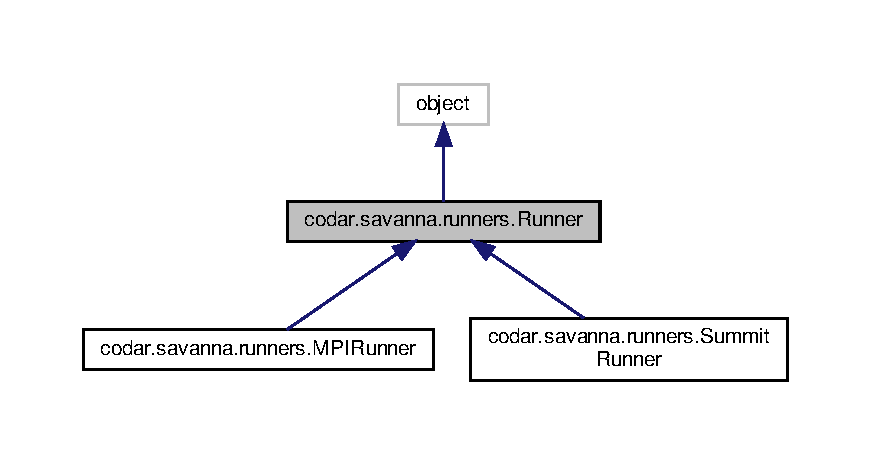
\includegraphics[width=350pt]{classcodar_1_1savanna_1_1runners_1_1_runner__inherit__graph}
\end{center}
\end{figure}


Collaboration diagram for codar.\+savanna.\+runners.\+Runner\+:
\nopagebreak
\begin{figure}[H]
\begin{center}
\leavevmode
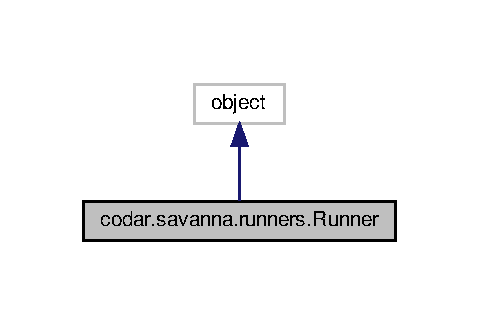
\includegraphics[width=230pt]{classcodar_1_1savanna_1_1runners_1_1_runner__coll__graph}
\end{center}
\end{figure}
\subsection*{Public Member Functions}
\begin{DoxyCompactItemize}
\item 
def \hyperlink{classcodar_1_1savanna_1_1runners_1_1_runner_a7e8a83cd991c604a5238af27bdc6e013}{wrap} (self, run, sched\+\_\+args)
\end{DoxyCompactItemize}


\subsection{Detailed Description}


Definition at line 6 of file runners.\+py.



\subsection{Member Function Documentation}
\mbox{\Hypertarget{classcodar_1_1savanna_1_1runners_1_1_runner_a7e8a83cd991c604a5238af27bdc6e013}\label{classcodar_1_1savanna_1_1runners_1_1_runner_a7e8a83cd991c604a5238af27bdc6e013}} 
\index{codar\+::savanna\+::runners\+::\+Runner@{codar\+::savanna\+::runners\+::\+Runner}!wrap@{wrap}}
\index{wrap@{wrap}!codar\+::savanna\+::runners\+::\+Runner@{codar\+::savanna\+::runners\+::\+Runner}}
\subsubsection{\texorpdfstring{wrap()}{wrap()}}
{\footnotesize\ttfamily def codar.\+savanna.\+runners.\+Runner.\+wrap (\begin{DoxyParamCaption}\item[{}]{self,  }\item[{}]{run,  }\item[{}]{sched\+\_\+args }\end{DoxyParamCaption})}



Definition at line 7 of file runners.\+py.



The documentation for this class was generated from the following file\+:\begin{DoxyCompactItemize}
\item 
savanna/\hyperlink{savanna_2runners_8py}{runners.\+py}\end{DoxyCompactItemize}

\hypertarget{classcodar_1_1savanna_1_1exc_1_1_savanna_exception}{}\section{codar.\+savanna.\+exc.\+Savanna\+Exception Class Reference}
\label{classcodar_1_1savanna_1_1exc_1_1_savanna_exception}\index{codar.\+savanna.\+exc.\+Savanna\+Exception@{codar.\+savanna.\+exc.\+Savanna\+Exception}}


Inheritance diagram for codar.\+savanna.\+exc.\+Savanna\+Exception\+:
\nopagebreak
\begin{figure}[H]
\begin{center}
\leavevmode
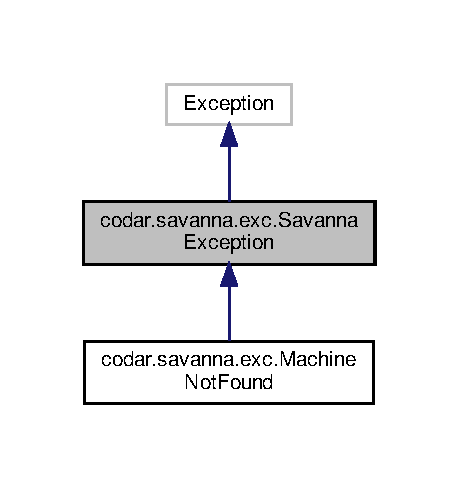
\includegraphics[width=220pt]{classcodar_1_1savanna_1_1exc_1_1_savanna_exception__inherit__graph}
\end{center}
\end{figure}


Collaboration diagram for codar.\+savanna.\+exc.\+Savanna\+Exception\+:
\nopagebreak
\begin{figure}[H]
\begin{center}
\leavevmode
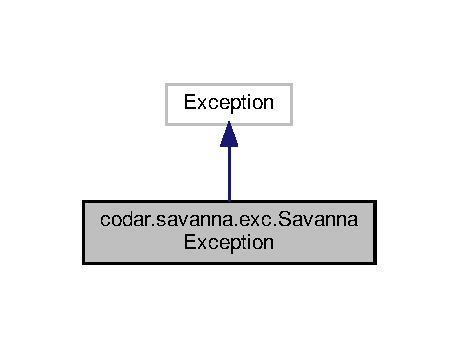
\includegraphics[width=220pt]{classcodar_1_1savanna_1_1exc_1_1_savanna_exception__coll__graph}
\end{center}
\end{figure}


\subsection{Detailed Description}


Definition at line 6 of file exc.\+py.



The documentation for this class was generated from the following file\+:\begin{DoxyCompactItemize}
\item 
\hyperlink{exc_8py}{exc.\+py}\end{DoxyCompactItemize}

\hypertarget{classcodar_1_1savanna_1_1machines_1_1_summit_node}{}\section{codar.\+savanna.\+machines.\+Summit\+Node Class Reference}
\label{classcodar_1_1savanna_1_1machines_1_1_summit_node}\index{codar.\+savanna.\+machines.\+Summit\+Node@{codar.\+savanna.\+machines.\+Summit\+Node}}


Inheritance diagram for codar.\+savanna.\+machines.\+Summit\+Node\+:
\nopagebreak
\begin{figure}[H]
\begin{center}
\leavevmode
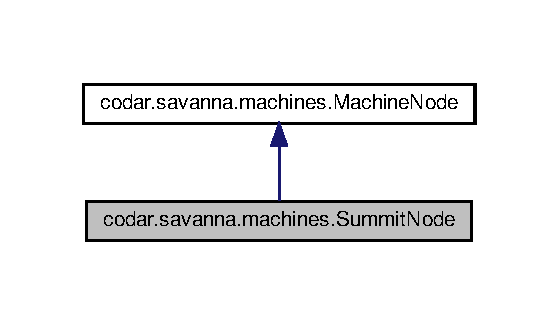
\includegraphics[width=268pt]{classcodar_1_1savanna_1_1machines_1_1_summit_node__inherit__graph}
\end{center}
\end{figure}


Collaboration diagram for codar.\+savanna.\+machines.\+Summit\+Node\+:
\nopagebreak
\begin{figure}[H]
\begin{center}
\leavevmode
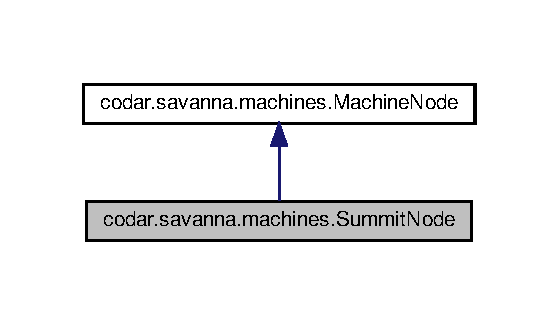
\includegraphics[width=268pt]{classcodar_1_1savanna_1_1machines_1_1_summit_node__coll__graph}
\end{center}
\end{figure}
\subsection*{Public Member Functions}
\begin{DoxyCompactItemize}
\item 
\mbox{\Hypertarget{classcodar_1_1savanna_1_1machines_1_1_summit_node_acc0c2a15d2204b3d5f547200fd4d055f}\label{classcodar_1_1savanna_1_1machines_1_1_summit_node_acc0c2a15d2204b3d5f547200fd4d055f}} 
def {\bfseries \+\_\+\+\_\+init\+\_\+\+\_\+} (self)
\item 
def \hyperlink{classcodar_1_1savanna_1_1machines_1_1_summit_node_a3360461b2a21624400e0ecdf052c8447}{validate\+\_\+layout} (self)
\item 
\mbox{\Hypertarget{classcodar_1_1savanna_1_1machines_1_1_summit_node_a7db80709d8a4ebc806559a03b9be8b68}\label{classcodar_1_1savanna_1_1machines_1_1_summit_node_a7db80709d8a4ebc806559a03b9be8b68}} 
def {\bfseries to\+\_\+json} (self)
\end{DoxyCompactItemize}
\subsection*{Additional Inherited Members}


\subsection{Member Function Documentation}
\mbox{\Hypertarget{classcodar_1_1savanna_1_1machines_1_1_summit_node_a3360461b2a21624400e0ecdf052c8447}\label{classcodar_1_1savanna_1_1machines_1_1_summit_node_a3360461b2a21624400e0ecdf052c8447}} 
\index{codar\+::savanna\+::machines\+::\+Summit\+Node@{codar\+::savanna\+::machines\+::\+Summit\+Node}!validate\+\_\+layout@{validate\+\_\+layout}}
\index{validate\+\_\+layout@{validate\+\_\+layout}!codar\+::savanna\+::machines\+::\+Summit\+Node@{codar\+::savanna\+::machines\+::\+Summit\+Node}}
\subsubsection{\texorpdfstring{validate\+\_\+layout()}{validate\_layout()}}
{\footnotesize\ttfamily def codar.\+savanna.\+machines.\+Summit\+Node.\+validate\+\_\+layout (\begin{DoxyParamCaption}\item[{}]{self }\end{DoxyParamCaption})}

\begin{DoxyVerb}Check that 1) the same rank of the same code is not repeated,
2) a gpu is not mapped to multiple executables.\end{DoxyVerb}
 

The documentation for this class was generated from the following file\+:\begin{DoxyCompactItemize}
\item 
machines.\+py\end{DoxyCompactItemize}

\hypertarget{classcodar_1_1savanna_1_1runners_1_1_summit_runner}{}\section{codar.\+savanna.\+runners.\+Summit\+Runner Class Reference}
\label{classcodar_1_1savanna_1_1runners_1_1_summit_runner}\index{codar.\+savanna.\+runners.\+Summit\+Runner@{codar.\+savanna.\+runners.\+Summit\+Runner}}


Inheritance diagram for codar.\+savanna.\+runners.\+Summit\+Runner\+:
\nopagebreak
\begin{figure}[H]
\begin{center}
\leavevmode
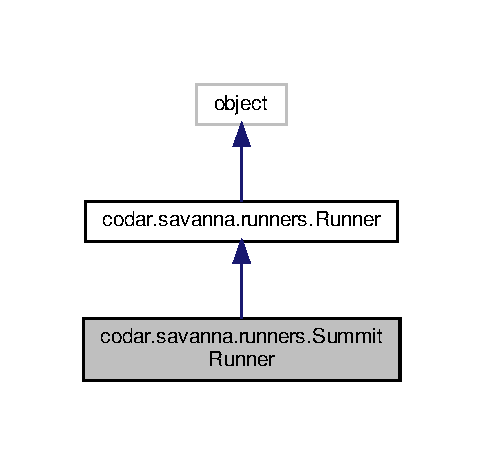
\includegraphics[width=232pt]{classcodar_1_1savanna_1_1runners_1_1_summit_runner__inherit__graph}
\end{center}
\end{figure}


Collaboration diagram for codar.\+savanna.\+runners.\+Summit\+Runner\+:
\nopagebreak
\begin{figure}[H]
\begin{center}
\leavevmode
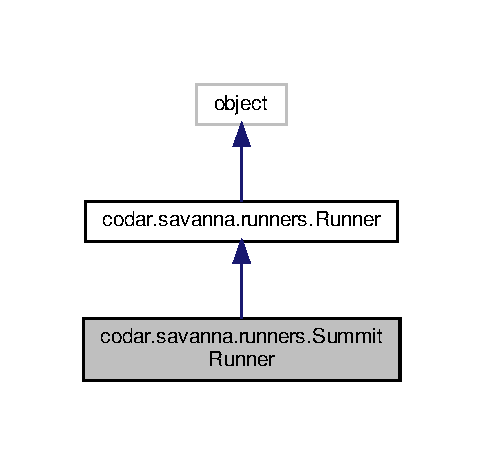
\includegraphics[width=232pt]{classcodar_1_1savanna_1_1runners_1_1_summit_runner__coll__graph}
\end{center}
\end{figure}
\subsection*{Public Member Functions}
\begin{DoxyCompactItemize}
\item 
def \hyperlink{classcodar_1_1savanna_1_1runners_1_1_summit_runner_ae02c57d99333e7987709dacee9bc1496}{\+\_\+\+\_\+init\+\_\+\+\_\+} (self)
\item 
def \hyperlink{classcodar_1_1savanna_1_1runners_1_1_summit_runner_ad754a3642a7d7e3dfcac4e6956ec9cbc}{wrap} (self, run, sched\+\_\+args)
\item 
def \hyperlink{classcodar_1_1savanna_1_1runners_1_1_summit_runner_a79042d5ab820ce5cc55292e2c3338994}{wrap\+\_\+deprecated} (self, run, jsrun\+\_\+opts, find\+\_\+in\+\_\+path=True)
\end{DoxyCompactItemize}
\subsection*{Public Attributes}
\begin{DoxyCompactItemize}
\item 
\hyperlink{classcodar_1_1savanna_1_1runners_1_1_summit_runner_a6dc6cbd63d546efb61ca8299bb186ec3}{exe}
\item 
\hyperlink{classcodar_1_1savanna_1_1runners_1_1_summit_runner_acaf90a041d1187271116f984ff8d0206}{nrs\+\_\+arg}
\item 
\hyperlink{classcodar_1_1savanna_1_1runners_1_1_summit_runner_a7ab533a9058a4575468d58026c169992}{tasks\+\_\+per\+\_\+rs\+\_\+arg}
\item 
\hyperlink{classcodar_1_1savanna_1_1runners_1_1_summit_runner_add0e4e1f69688a9aaaeb19dbeef50b1d}{cpus\+\_\+per\+\_\+rs\+\_\+arg}
\item 
\hyperlink{classcodar_1_1savanna_1_1runners_1_1_summit_runner_a10b2fdfd7b6b407ab4bc218ededcbc0a}{gpus\+\_\+per\+\_\+rs\+\_\+arg}
\item 
\hyperlink{classcodar_1_1savanna_1_1runners_1_1_summit_runner_ace56b0a9e2920543866021bb150a55a8}{rs\+\_\+per\+\_\+host\+\_\+arg}
\item 
\hyperlink{classcodar_1_1savanna_1_1runners_1_1_summit_runner_a0550589f1ba354d1a0fd645023153ec1}{launch\+\_\+distribution\+\_\+arg}
\item 
\hyperlink{classcodar_1_1savanna_1_1runners_1_1_summit_runner_a92e82ecf812eb3c701fc855cda464c38}{bind\+\_\+arg}
\item 
\hyperlink{classcodar_1_1savanna_1_1runners_1_1_summit_runner_a968e40e2579e317df88c8da777e7be0f}{machine}
\end{DoxyCompactItemize}


\subsection{Detailed Description}


Definition at line 44 of file runners.\+py.



\subsection{Constructor \& Destructor Documentation}
\mbox{\Hypertarget{classcodar_1_1savanna_1_1runners_1_1_summit_runner_ae02c57d99333e7987709dacee9bc1496}\label{classcodar_1_1savanna_1_1runners_1_1_summit_runner_ae02c57d99333e7987709dacee9bc1496}} 
\index{codar\+::savanna\+::runners\+::\+Summit\+Runner@{codar\+::savanna\+::runners\+::\+Summit\+Runner}!\+\_\+\+\_\+init\+\_\+\+\_\+@{\+\_\+\+\_\+init\+\_\+\+\_\+}}
\index{\+\_\+\+\_\+init\+\_\+\+\_\+@{\+\_\+\+\_\+init\+\_\+\+\_\+}!codar\+::savanna\+::runners\+::\+Summit\+Runner@{codar\+::savanna\+::runners\+::\+Summit\+Runner}}
\subsubsection{\texorpdfstring{\+\_\+\+\_\+init\+\_\+\+\_\+()}{\_\_init\_\_()}}
{\footnotesize\ttfamily def codar.\+savanna.\+runners.\+Summit\+Runner.\+\_\+\+\_\+init\+\_\+\+\_\+ (\begin{DoxyParamCaption}\item[{}]{self }\end{DoxyParamCaption})}



Definition at line 45 of file runners.\+py.



\subsection{Member Function Documentation}
\mbox{\Hypertarget{classcodar_1_1savanna_1_1runners_1_1_summit_runner_ad754a3642a7d7e3dfcac4e6956ec9cbc}\label{classcodar_1_1savanna_1_1runners_1_1_summit_runner_ad754a3642a7d7e3dfcac4e6956ec9cbc}} 
\index{codar\+::savanna\+::runners\+::\+Summit\+Runner@{codar\+::savanna\+::runners\+::\+Summit\+Runner}!wrap@{wrap}}
\index{wrap@{wrap}!codar\+::savanna\+::runners\+::\+Summit\+Runner@{codar\+::savanna\+::runners\+::\+Summit\+Runner}}
\subsubsection{\texorpdfstring{wrap()}{wrap()}}
{\footnotesize\ttfamily def codar.\+savanna.\+runners.\+Summit\+Runner.\+wrap (\begin{DoxyParamCaption}\item[{}]{self,  }\item[{}]{run,  }\item[{}]{sched\+\_\+args }\end{DoxyParamCaption})}



Definition at line 56 of file runners.\+py.

\mbox{\Hypertarget{classcodar_1_1savanna_1_1runners_1_1_summit_runner_a79042d5ab820ce5cc55292e2c3338994}\label{classcodar_1_1savanna_1_1runners_1_1_summit_runner_a79042d5ab820ce5cc55292e2c3338994}} 
\index{codar\+::savanna\+::runners\+::\+Summit\+Runner@{codar\+::savanna\+::runners\+::\+Summit\+Runner}!wrap\+\_\+deprecated@{wrap\+\_\+deprecated}}
\index{wrap\+\_\+deprecated@{wrap\+\_\+deprecated}!codar\+::savanna\+::runners\+::\+Summit\+Runner@{codar\+::savanna\+::runners\+::\+Summit\+Runner}}
\subsubsection{\texorpdfstring{wrap\+\_\+deprecated()}{wrap\_deprecated()}}
{\footnotesize\ttfamily def codar.\+savanna.\+runners.\+Summit\+Runner.\+wrap\+\_\+deprecated (\begin{DoxyParamCaption}\item[{}]{self,  }\item[{}]{run,  }\item[{}]{jsrun\+\_\+opts,  }\item[{}]{find\+\_\+in\+\_\+path = {\ttfamily True} }\end{DoxyParamCaption})}

\begin{DoxyVerb}This function is deprecated in favor of the above that uses erf
files\end{DoxyVerb}
 

Definition at line 60 of file runners.\+py.



\subsection{Member Data Documentation}
\mbox{\Hypertarget{classcodar_1_1savanna_1_1runners_1_1_summit_runner_a92e82ecf812eb3c701fc855cda464c38}\label{classcodar_1_1savanna_1_1runners_1_1_summit_runner_a92e82ecf812eb3c701fc855cda464c38}} 
\index{codar\+::savanna\+::runners\+::\+Summit\+Runner@{codar\+::savanna\+::runners\+::\+Summit\+Runner}!bind\+\_\+arg@{bind\+\_\+arg}}
\index{bind\+\_\+arg@{bind\+\_\+arg}!codar\+::savanna\+::runners\+::\+Summit\+Runner@{codar\+::savanna\+::runners\+::\+Summit\+Runner}}
\subsubsection{\texorpdfstring{bind\+\_\+arg}{bind\_arg}}
{\footnotesize\ttfamily codar.\+savanna.\+runners.\+Summit\+Runner.\+bind\+\_\+arg}



Definition at line 53 of file runners.\+py.

\mbox{\Hypertarget{classcodar_1_1savanna_1_1runners_1_1_summit_runner_add0e4e1f69688a9aaaeb19dbeef50b1d}\label{classcodar_1_1savanna_1_1runners_1_1_summit_runner_add0e4e1f69688a9aaaeb19dbeef50b1d}} 
\index{codar\+::savanna\+::runners\+::\+Summit\+Runner@{codar\+::savanna\+::runners\+::\+Summit\+Runner}!cpus\+\_\+per\+\_\+rs\+\_\+arg@{cpus\+\_\+per\+\_\+rs\+\_\+arg}}
\index{cpus\+\_\+per\+\_\+rs\+\_\+arg@{cpus\+\_\+per\+\_\+rs\+\_\+arg}!codar\+::savanna\+::runners\+::\+Summit\+Runner@{codar\+::savanna\+::runners\+::\+Summit\+Runner}}
\subsubsection{\texorpdfstring{cpus\+\_\+per\+\_\+rs\+\_\+arg}{cpus\_per\_rs\_arg}}
{\footnotesize\ttfamily codar.\+savanna.\+runners.\+Summit\+Runner.\+cpus\+\_\+per\+\_\+rs\+\_\+arg}



Definition at line 49 of file runners.\+py.

\mbox{\Hypertarget{classcodar_1_1savanna_1_1runners_1_1_summit_runner_a6dc6cbd63d546efb61ca8299bb186ec3}\label{classcodar_1_1savanna_1_1runners_1_1_summit_runner_a6dc6cbd63d546efb61ca8299bb186ec3}} 
\index{codar\+::savanna\+::runners\+::\+Summit\+Runner@{codar\+::savanna\+::runners\+::\+Summit\+Runner}!exe@{exe}}
\index{exe@{exe}!codar\+::savanna\+::runners\+::\+Summit\+Runner@{codar\+::savanna\+::runners\+::\+Summit\+Runner}}
\subsubsection{\texorpdfstring{exe}{exe}}
{\footnotesize\ttfamily codar.\+savanna.\+runners.\+Summit\+Runner.\+exe}



Definition at line 46 of file runners.\+py.

\mbox{\Hypertarget{classcodar_1_1savanna_1_1runners_1_1_summit_runner_a10b2fdfd7b6b407ab4bc218ededcbc0a}\label{classcodar_1_1savanna_1_1runners_1_1_summit_runner_a10b2fdfd7b6b407ab4bc218ededcbc0a}} 
\index{codar\+::savanna\+::runners\+::\+Summit\+Runner@{codar\+::savanna\+::runners\+::\+Summit\+Runner}!gpus\+\_\+per\+\_\+rs\+\_\+arg@{gpus\+\_\+per\+\_\+rs\+\_\+arg}}
\index{gpus\+\_\+per\+\_\+rs\+\_\+arg@{gpus\+\_\+per\+\_\+rs\+\_\+arg}!codar\+::savanna\+::runners\+::\+Summit\+Runner@{codar\+::savanna\+::runners\+::\+Summit\+Runner}}
\subsubsection{\texorpdfstring{gpus\+\_\+per\+\_\+rs\+\_\+arg}{gpus\_per\_rs\_arg}}
{\footnotesize\ttfamily codar.\+savanna.\+runners.\+Summit\+Runner.\+gpus\+\_\+per\+\_\+rs\+\_\+arg}



Definition at line 50 of file runners.\+py.

\mbox{\Hypertarget{classcodar_1_1savanna_1_1runners_1_1_summit_runner_a0550589f1ba354d1a0fd645023153ec1}\label{classcodar_1_1savanna_1_1runners_1_1_summit_runner_a0550589f1ba354d1a0fd645023153ec1}} 
\index{codar\+::savanna\+::runners\+::\+Summit\+Runner@{codar\+::savanna\+::runners\+::\+Summit\+Runner}!launch\+\_\+distribution\+\_\+arg@{launch\+\_\+distribution\+\_\+arg}}
\index{launch\+\_\+distribution\+\_\+arg@{launch\+\_\+distribution\+\_\+arg}!codar\+::savanna\+::runners\+::\+Summit\+Runner@{codar\+::savanna\+::runners\+::\+Summit\+Runner}}
\subsubsection{\texorpdfstring{launch\+\_\+distribution\+\_\+arg}{launch\_distribution\_arg}}
{\footnotesize\ttfamily codar.\+savanna.\+runners.\+Summit\+Runner.\+launch\+\_\+distribution\+\_\+arg}



Definition at line 52 of file runners.\+py.

\mbox{\Hypertarget{classcodar_1_1savanna_1_1runners_1_1_summit_runner_a968e40e2579e317df88c8da777e7be0f}\label{classcodar_1_1savanna_1_1runners_1_1_summit_runner_a968e40e2579e317df88c8da777e7be0f}} 
\index{codar\+::savanna\+::runners\+::\+Summit\+Runner@{codar\+::savanna\+::runners\+::\+Summit\+Runner}!machine@{machine}}
\index{machine@{machine}!codar\+::savanna\+::runners\+::\+Summit\+Runner@{codar\+::savanna\+::runners\+::\+Summit\+Runner}}
\subsubsection{\texorpdfstring{machine}{machine}}
{\footnotesize\ttfamily codar.\+savanna.\+runners.\+Summit\+Runner.\+machine}



Definition at line 54 of file runners.\+py.

\mbox{\Hypertarget{classcodar_1_1savanna_1_1runners_1_1_summit_runner_acaf90a041d1187271116f984ff8d0206}\label{classcodar_1_1savanna_1_1runners_1_1_summit_runner_acaf90a041d1187271116f984ff8d0206}} 
\index{codar\+::savanna\+::runners\+::\+Summit\+Runner@{codar\+::savanna\+::runners\+::\+Summit\+Runner}!nrs\+\_\+arg@{nrs\+\_\+arg}}
\index{nrs\+\_\+arg@{nrs\+\_\+arg}!codar\+::savanna\+::runners\+::\+Summit\+Runner@{codar\+::savanna\+::runners\+::\+Summit\+Runner}}
\subsubsection{\texorpdfstring{nrs\+\_\+arg}{nrs\_arg}}
{\footnotesize\ttfamily codar.\+savanna.\+runners.\+Summit\+Runner.\+nrs\+\_\+arg}



Definition at line 47 of file runners.\+py.

\mbox{\Hypertarget{classcodar_1_1savanna_1_1runners_1_1_summit_runner_ace56b0a9e2920543866021bb150a55a8}\label{classcodar_1_1savanna_1_1runners_1_1_summit_runner_ace56b0a9e2920543866021bb150a55a8}} 
\index{codar\+::savanna\+::runners\+::\+Summit\+Runner@{codar\+::savanna\+::runners\+::\+Summit\+Runner}!rs\+\_\+per\+\_\+host\+\_\+arg@{rs\+\_\+per\+\_\+host\+\_\+arg}}
\index{rs\+\_\+per\+\_\+host\+\_\+arg@{rs\+\_\+per\+\_\+host\+\_\+arg}!codar\+::savanna\+::runners\+::\+Summit\+Runner@{codar\+::savanna\+::runners\+::\+Summit\+Runner}}
\subsubsection{\texorpdfstring{rs\+\_\+per\+\_\+host\+\_\+arg}{rs\_per\_host\_arg}}
{\footnotesize\ttfamily codar.\+savanna.\+runners.\+Summit\+Runner.\+rs\+\_\+per\+\_\+host\+\_\+arg}



Definition at line 51 of file runners.\+py.

\mbox{\Hypertarget{classcodar_1_1savanna_1_1runners_1_1_summit_runner_a7ab533a9058a4575468d58026c169992}\label{classcodar_1_1savanna_1_1runners_1_1_summit_runner_a7ab533a9058a4575468d58026c169992}} 
\index{codar\+::savanna\+::runners\+::\+Summit\+Runner@{codar\+::savanna\+::runners\+::\+Summit\+Runner}!tasks\+\_\+per\+\_\+rs\+\_\+arg@{tasks\+\_\+per\+\_\+rs\+\_\+arg}}
\index{tasks\+\_\+per\+\_\+rs\+\_\+arg@{tasks\+\_\+per\+\_\+rs\+\_\+arg}!codar\+::savanna\+::runners\+::\+Summit\+Runner@{codar\+::savanna\+::runners\+::\+Summit\+Runner}}
\subsubsection{\texorpdfstring{tasks\+\_\+per\+\_\+rs\+\_\+arg}{tasks\_per\_rs\_arg}}
{\footnotesize\ttfamily codar.\+savanna.\+runners.\+Summit\+Runner.\+tasks\+\_\+per\+\_\+rs\+\_\+arg}



Definition at line 48 of file runners.\+py.



The documentation for this class was generated from the following file\+:\begin{DoxyCompactItemize}
\item 
\hyperlink{runners_8py}{runners.\+py}\end{DoxyCompactItemize}

\hypertarget{classcodar_1_1savanna_1_1status_1_1_workflow_status}{}\section{codar.\+savanna.\+status.\+Workflow\+Status Class Reference}
\label{classcodar_1_1savanna_1_1status_1_1_workflow_status}\index{codar.\+savanna.\+status.\+Workflow\+Status@{codar.\+savanna.\+status.\+Workflow\+Status}}


Inheritance diagram for codar.\+savanna.\+status.\+Workflow\+Status\+:
\nopagebreak
\begin{figure}[H]
\begin{center}
\leavevmode
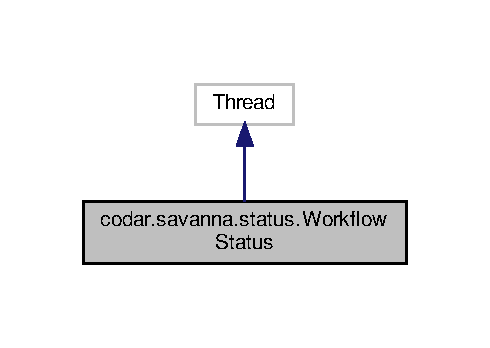
\includegraphics[width=235pt]{classcodar_1_1savanna_1_1status_1_1_workflow_status__inherit__graph}
\end{center}
\end{figure}


Collaboration diagram for codar.\+savanna.\+status.\+Workflow\+Status\+:
\nopagebreak
\begin{figure}[H]
\begin{center}
\leavevmode
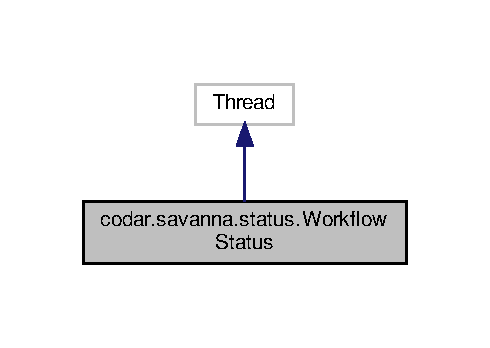
\includegraphics[width=235pt]{classcodar_1_1savanna_1_1status_1_1_workflow_status__coll__graph}
\end{center}
\end{figure}
\subsection*{Public Member Functions}
\begin{DoxyCompactItemize}
\item 
def \hyperlink{classcodar_1_1savanna_1_1status_1_1_workflow_status_a8e9bfa3627135919e28b501dde60241c}{\+\_\+\+\_\+init\+\_\+\+\_\+} (self, \hyperlink{classcodar_1_1savanna_1_1status_1_1_workflow_status_ae4eb41515ae3ac77a11e1905835497e6}{file\+\_\+path})
\item 
def \hyperlink{classcodar_1_1savanna_1_1status_1_1_workflow_status_a66a2494ce4cb8605df72cf480e756e08}{set\+\_\+state} (self, pipeline\+\_\+state)
\end{DoxyCompactItemize}
\subsection*{Public Attributes}
\begin{DoxyCompactItemize}
\item 
\hyperlink{classcodar_1_1savanna_1_1status_1_1_workflow_status_ae4eb41515ae3ac77a11e1905835497e6}{file\+\_\+path}
\end{DoxyCompactItemize}


\subsection{Detailed Description}


Definition at line 24 of file status.\+py.



\subsection{Constructor \& Destructor Documentation}
\mbox{\Hypertarget{classcodar_1_1savanna_1_1status_1_1_workflow_status_a8e9bfa3627135919e28b501dde60241c}\label{classcodar_1_1savanna_1_1status_1_1_workflow_status_a8e9bfa3627135919e28b501dde60241c}} 
\index{codar\+::savanna\+::status\+::\+Workflow\+Status@{codar\+::savanna\+::status\+::\+Workflow\+Status}!\+\_\+\+\_\+init\+\_\+\+\_\+@{\+\_\+\+\_\+init\+\_\+\+\_\+}}
\index{\+\_\+\+\_\+init\+\_\+\+\_\+@{\+\_\+\+\_\+init\+\_\+\+\_\+}!codar\+::savanna\+::status\+::\+Workflow\+Status@{codar\+::savanna\+::status\+::\+Workflow\+Status}}
\subsubsection{\texorpdfstring{\+\_\+\+\_\+init\+\_\+\+\_\+()}{\_\_init\_\_()}}
{\footnotesize\ttfamily def codar.\+savanna.\+status.\+Workflow\+Status.\+\_\+\+\_\+init\+\_\+\+\_\+ (\begin{DoxyParamCaption}\item[{}]{self,  }\item[{}]{file\+\_\+path }\end{DoxyParamCaption})}



Definition at line 25 of file status.\+py.



\subsection{Member Function Documentation}
\mbox{\Hypertarget{classcodar_1_1savanna_1_1status_1_1_workflow_status_a66a2494ce4cb8605df72cf480e756e08}\label{classcodar_1_1savanna_1_1status_1_1_workflow_status_a66a2494ce4cb8605df72cf480e756e08}} 
\index{codar\+::savanna\+::status\+::\+Workflow\+Status@{codar\+::savanna\+::status\+::\+Workflow\+Status}!set\+\_\+state@{set\+\_\+state}}
\index{set\+\_\+state@{set\+\_\+state}!codar\+::savanna\+::status\+::\+Workflow\+Status@{codar\+::savanna\+::status\+::\+Workflow\+Status}}
\subsubsection{\texorpdfstring{set\+\_\+state()}{set\_state()}}
{\footnotesize\ttfamily def codar.\+savanna.\+status.\+Workflow\+Status.\+set\+\_\+state (\begin{DoxyParamCaption}\item[{}]{self,  }\item[{}]{pipeline\+\_\+state }\end{DoxyParamCaption})}



Definition at line 37 of file status.\+py.



\subsection{Member Data Documentation}
\mbox{\Hypertarget{classcodar_1_1savanna_1_1status_1_1_workflow_status_ae4eb41515ae3ac77a11e1905835497e6}\label{classcodar_1_1savanna_1_1status_1_1_workflow_status_ae4eb41515ae3ac77a11e1905835497e6}} 
\index{codar\+::savanna\+::status\+::\+Workflow\+Status@{codar\+::savanna\+::status\+::\+Workflow\+Status}!file\+\_\+path@{file\+\_\+path}}
\index{file\+\_\+path@{file\+\_\+path}!codar\+::savanna\+::status\+::\+Workflow\+Status@{codar\+::savanna\+::status\+::\+Workflow\+Status}}
\subsubsection{\texorpdfstring{file\+\_\+path}{file\_path}}
{\footnotesize\ttfamily codar.\+savanna.\+status.\+Workflow\+Status.\+file\+\_\+path}



Definition at line 27 of file status.\+py.



The documentation for this class was generated from the following file\+:\begin{DoxyCompactItemize}
\item 
savanna/\hyperlink{savanna_2status_8py}{status.\+py}\end{DoxyCompactItemize}

%--- End generated contents ---

% Index
\backmatter
\newpage
\phantomsection
\clearemptydoublepage
\addcontentsline{toc}{chapter}{Index}
\printindex

\end{document}
